\documentclass[final,12pt]{colt2018} % Anonymized submission
% \documentclass{colt2017} % Include author names

% The following packages will be automatically loaded:
% amsmath, amssymb, natbib, graphicx, url, algorithm2e

\title[Accelerating Stochastic Gradient Descent]{Accelerating Stochastic Gradient Descent for Least Squares Regression}
\usepackage{times}
% The following packages will be automatically loaded:
% url, algorithm2e
% For figures
%\usepackage{authblk}

%\usepackage{amsthm,fullpage}
\usepackage{flushend,multicol,adjustbox}
% For citations
\usepackage{pifont,color}
%\usepackage{placeins}
%\usepackage{subcaption}
% For algorithms
%\usepackage{algorithm}
%\usepackage[ruled]{algorithm2e}algorithmic,
%\usepackage[aboveskip=0pt]{caption}
\usepackage{algorithm,bm,multirow,array}
\usepackage{enumitem,scalerel}
\usepackage{xcolor,hyperref}
\graphicspath{{figures/newer-figs/}}

 % Use \Name{Author Name} to specify the name.
 % If the surname contains spaces, enclose the surname
 % in braces, e.g. \Name{John {Smith Jones}} similarly
 % if the name has a "von" part, e.g \Name{Jane {de Winter}}.
 % If the first letter in the forenames is a diacritic
 % enclose the diacritic in braces, e.g. \Name{{\'E}louise Smith}

 % Two authors with the same address
\coltauthor{\Name{Prateek Jain}\Email{prajain@microsoft.com}\\
\Name{Praneeth Netrapalli}\Email{praneeth@microsoft.com}\\
\addr Microsoft Research, Bangalore, India
\AND
\Name{Sham M. Kakade} \Email{sham@cs.washington.edu}\\
\Name{Rahul Kidambi} \Email{rkidambi@uw.edu}\\
\addr University of Washington, Seattle, WA, USA
\AND
\Name{Aaron Sidford} \Email{sidford@stanford.com}\\
\addr Stanford University, Palo Alto, CA, USA
}
 % Three or more authors with the same address:
 % \coltauthor{\Name{Author Name1} \Email{an1@sample.com}\\
 %  \Name{Author Name2} \Email{an2@sample.com}\\
 %  \Name{Author Name3} \Email{an3@sample.com}\\
 %  \addr Address}


 % Authors with different addresses:
 \iffalse
 \coltauthor{\Name{Author Name1} \Email{abc@sample.com}\\
 \addr Address 1
 \AND
 \Name{Author Name2} \Email{xyz@sample.com}\\
 \addr Address 2
 }
\fi
\iffalse
 \coltauthor{\Name{Prateek Jain} \Email{prajain@microsoft.com}\\
%	\AND
	\Name{Sham M. Kakade} \Email{sham@cs.washington.edu}\\
%	\AND
	\Name{Rahul Kidambi} \Email{rkidambi@uw.edu}\\
%	\AND
	\Name{Praneeth Netrapalli} \Email{praneeth@microsoft.com}\\
%	\AND
	\Name{Aaron Sidford} \Email{sidford@stanford.edu}
}
\fi
\iffalse
\renewcommand\Authfont{\fontsize{11}{14}\selectfont}
\renewcommand\Affilfont{\fontsize{9}{10.8}}
\author[1]{Prateek Jain}
\author[2]{Sham M. Kakade}
\author[2]{Rahul Kidambi}
\author[1]{Praneeth Netrapalli}
\author[3]{Aaron Sidford}
\affil[1]{Microsoft Research, Bangalore.    \url{{prajain,praneeth}@microsoft.com}}
\affil[2]{University of Washington, Seattle, WA.  \url{sham@cs.washington.edu},\ \url{rkidambi@uw.edu}}
\affil[3]{Stanford University, Palo Alto, CA. \url{sidford@stanford.edu}.}
\fi
% Custom commands
\newcommand{\bR}{\mathbb{R}}
\newcommand{\mL}{\mathcal{L}}
\newcommand{\mO}{\mathcal{O}}
\newcommand{\mG}{\mathcal{G}}
\newcommand{\mF}{\mathcal{F}}
\newcommand{\mP}{\mathcal{P}}
\newcommand{\mR}{\mathcal{R}}
\newcommand{\bI}{\mathbf{1}}
\newcommand{\TV}{d_{\text{TV}}}
\newcommand{\KL}{d_{\text{KL}}}
\newcommand{\Tr}{\text{Tr}}
\newcommand{\bP}{\mathbb{P}}
\newcommand{\bE}{\mathbb{E}}

\newcommand{\N}{\mathcal{N}}
\newcommand{\Id}{\mathsf{I}}
\newcommand{\las}{\mathsf{las}}
\newcommand{\spca}{\mathsf{spca}}

\newcommand{\Yt}{\widetilde{Y}}
\newcommand{\Wt}{\widetilde{W}}


% Standard environments
%\newtheorem{definition}{Definition}[section]
%\newtheorem{example}{Example}[section]
%\newtheorem{exercise}{Exercise}[section]
\newtheorem{fact}{Fact}[section]
%\newtheorem{theorem}{Theorem}[section]
%\newtheorem{corollary}{Corollary}[section]
%\newtheorem{conjecture}{Conjecture}[section]
%\newtheorem{lemma}{Lemma}[section]
%\newtheorem{problem}{Problem}[section]
\newenvironment{solution}[1][Solution]{
    \begin{proof}[#1]
  }{
    \end{proof}
  }

\newenvironment{fminipage}%
  {\begin{Sbox}\begin{minipage}}%
  {\end{minipage}\end{Sbox}\fbox{\TheSbox}}

\newenvironment{algbox}[0]{\vskip 0.2in
\noindent 
 \begin{fminipage}{5.9in}
}{
\end{fminipage}
\vskip 0.2in
}

\setcounter{tocdepth}{1}
\allowdisplaybreaks

\begin{document}


\maketitle

\begin{abstract}
	

There is widespread sentiment that fast gradient methods (\emph{e.g.}
Nesterov's acceleration, conjugate gradient, heavy ball) are not
effective for the purposes of stochastic optimization due to their
instability and error accumulation. Numerous works have attempted to
quantify these instabilities in the face of either statistical or
non-statistical
errors~\citep{Paige71,Proakis74,Polyak87,Greenbaum89,DevolderGN14}.
This work considers these issues for the special case of
stochastic approximation for the least squares regression problem, and
our main result refutes this conventional wisdom by showing that
acceleration can be made robust to statistical errors.  In
particular, this work introduces an accelerated stochastic gradient
method that provably achieves the minimax optimal statistical risk
faster than stochastic gradient descent.  Critical to the analysis is
a sharp characterization of accelerated stochastic gradient descent as
a stochastic process. We hope this characterization gives insights
towards the broader question of designing simple and effective
accelerated stochastic methods for more general convex and non-convex
optimization problems.


\iffalse
There is widespread sentiment that fast gradient methods (\emph{e.g.}
Nesterov's acceleration, conjugate gradient, heavy ball) are not
effective for the purposes of stochastic optimization due to their
instability and error accumulation, a notion made precise
in~\cite{dAspremont08,DevolderGN14}.  This work considers the use of
fast gradient methods for the special case of stochastic approximation for the
least squares regression problem.  Our main
result refutes the conventional wisdom by showing that acceleration can
be made robust to \emph{statistical} errors.  In particular, this work
introduces an accelerated stochastic gradient method that provably
achieves the minimax optimal statistical risk faster than stochastic
gradient descent.  Critical to the analysis is a sharp
characterization of accelerated stochastic gradient descent as a
stochastic process. We hope this characterization gives insights
towards the broader question of designing simple and effective
accelerated stochastic methods for more general convex and non-convex
optimization problems.
\fi
\end{abstract}

\begin{keywords}
	Stochastic Approximation, Acceleration, Stochastic Gradient Descent, Accelerated Stochastic Gradient Descent, Least Squares Regression.
\end{keywords}

\section{Introduction}

Stochastic gradient descent (SGD) is the workhorse algorithm for
optimization in machine learning and stochastic approximation
problems; improving its runtime dependencies is a central issue in
large scale stochastic optimization that often arise in machine 
learning problems at scale~\citep{BottouB07}, where one can only resort to streaming algorithms. 

%Unfortunately, the folklore is that it is not possible to utilize fast gradient methods for stochastic optimization due to their instability and error accumulation.  This work strongly refutes this folklore showing, in very strong sense, that acceleration is robust to \emph{statistical} errors. In particular, we provide an accelerated stochastic gradient descent algorithm that enjoys minimax optimal statistical estimation at rate that is provably faster than stochastic gradient descent.

This work examines these broader runtime issues for the special case of stochastic approximation in the
following least squares regression problem:% (i.e. linear regression) \sidford{Not sure need the i.e. and would get a better line break. Also changed formatting of the 1/2 below}:
\vspace{-0.2cm}
\begin{align}
\label{eq:objFun}
\min_{\x \in \R^d} P(\x), \, \, \, 
\text{where, }P(\x)\defeq \tfrac{1}{2} \cdot\Eover{\distr}{(b-\iprod{\x}{\a})^2},
\end{align}

\vspace{-0.3cm}
\noindent where we have access to a {\em stochastic first order oracle}, which, when provided with $\x$ as an input, returns a noisy unbiased stochastic gradient using a tuple $(\a,\b)$ sampled from $\D(\R^d\times \R)$, with $d$ being the dimension of the problem. A query to the stochastic first-order oracle at $\x$ produces: %an unbiased estimate $\widehat{\nabla}P(\x)$ of the gradient $\nabla P(x)$ of the form 
\vspace{-0.25cm}
\begin{align}
\label{eq:stochFirstOrderOracle}
\widehat{\nabla}P(\x) = \ -(b-\iprod{\a}{\x})\cdot\a.% \quad \text{where, }\E{\widehat{\nabla}P(\x)}=\nabla P(\x)\quad\text{({\em unbiased} estimate)}.
\end{align}
Note $\E{\widehat{\nabla}P(\x)}=\nabla P(\x)$ (i.e. eq\eqref{eq:stochFirstOrderOracle} is an unbiased estimate). Note that nearly all practical stochastic algorithms use sampled gradients of the specific form as in equation~\ref{eq:stochFirstOrderOracle}. We discuss differences to the more general stochastic first order oracle~\citep{NemirovskyY83} in section~\ref{sec:related}.

\begin{table*}[t]
	\begin{center}
  \begin{adjustbox}{max width=\textwidth}
  		\begin{tabular}{| c | c | c | c |}
			\hline
			Algorithm & Final error & Runtime & Memory\\ 
		\hline
			\begin{tabular}{@{}c@{}} Accelerated SVRG \\ \citep{Zhu16} \end{tabular}&  $\mathcal{O}\left(\frac{\sigma^2 d}{n}\right)$ & $({n+\sqrt{n\cnH}})d\log\bigg({\frac{P(\xt[0])-P(\xt[*])}{(\sigma^2d/n)}}\bigg)$ &$nd$\\
			\hline
			\begin{tabular}{@{}c@{}} Streaming SVRG \\ \citep{FrostigGKS15} \\ 	Iterate Averaged SGD \\ \citep{JainKKNS16} \end{tabular} & $\mathcal{O}\left(\exp\left(\frac{-n}{\cnH}\right)\cdot\big(P(\xt[0])-P(\xt[*])\big) + \frac{\sigma^2 d}{n}\right)$ & ${nd}$ &$\mathcal{O}(d)$\\
\hline
			\begin{tabular}{@{}c@{}} Accelerated Stochastic Gradient Descent \\ (this paper) \end{tabular}& $\mathcal{O}^*\left(\exp\left(\frac{-n}{\sqrt{\cnH\cnS}}\right) \big(P(\xt[0])-P(\xt[*])\big)\right) + \mathcal{O}\left(\frac{\sigma^2 d}{n}\right)$ & ${nd}$ &$\mathcal{O}(d)$\\
			\hline
		\end{tabular} 
		\end{adjustbox}
				\caption{Comparison of this work to the best known non-asymptotic results~\citep{FrostigGKS15,JainKKNS16} for the least squares stochastic approximation problem.\iffalse See section~\ref{sec:related} for related work.\fi\ Here, $d,n$ are the problem dimension, number of samples; $\cnH$, $\cnS$ denote the condition number and statistical condition number of the distribution; $\sigma^2$, $P(\xt[0])-P(\xt[*])$ denote the noise level and initial excess risk, $\mathcal{O}^*$ hides lower order terms in $d,\cnH,\cnS$ (see section~\ref{sec:prob} for definitions and a proof for $\cnS \leq \cnH$). Note that Accelerated SVRG~\citep{Zhu16} is not a streaming algorithm. 
                  %For the least squares stochastic approximation problem, there are several
                  %non-asymptotic
                  %analyses~\citep{BachM13,DefossezB15,NeedellSW16,FrostigGKS15,JainKKNS16},
                  %and we refer to the fastest rates in this table. 
                }\vspace*{-1cm}
		\iffalse\caption{Comparison of this work to the best known prior non-asymptotic results~\citep{BachM13,DefossezB15,NeedellSW16,FrostigGKS15,JainKKNS16} for the least squares stochastic approximation problem. Here, $d,n$ are the problem dimension, number of samples;
                  $\cnH$, $\cnS$ denote the condition number and
                  statistical condition number of the distribution,
                  $\sigma^2$ denotes the noise level, and
                  $P(\xt[0])-P(\xt[*])$ denotes the initial excess
                  risk, and $\mathcal{O}^*$ hides lower order terms in
                  $d,\cnH,\cnS$ (see section~\ref{sec:prob} for definitions and a short proof that $\cnS \leq \cnH$). Note that Accelerated SVRG~\citep{Zhu16} is not a streaming algorithm. See section~\ref{sec:related} for related work.
                  %For the least squares stochastic approximation problem, there are several
                  %non-asymptotic
                  %analyses~\citep{BachM13,DefossezB15,NeedellSW16,FrostigGKS15,JainKKNS16},
                  %and we refer to the fastest rates in this table. 
                }\fi
		\label{tab:comp}
	\end{center}
\end{table*}
Let $\xs \eqdef \arg\min_\x P(\x)$ be a population risk minimizer.  Given any estimation procedure which returns $\xhat_n $ using $n$ samples, define the {\em excess risk} (which we also refer to as the \emph{generalization error} or the \emph{error}) of $\xhat_n$ as $\E{P(\xhat_n)}-P(\xs)$.
Now, equipped a stochastic first-order oracle (equation~\eqref{eq:stochFirstOrderOracle}), our goal is to provide a computationally efficient (and streaming) estimation method whose excess risk is comparable to the optimal statistical minimax rate.  

In the limit of large $n$, this minimax rate is achieved by the {\em empirical risk minimizer} (ERM), which is defined as follows. Given $n$ i.i.d. samples $\ST_n=\{(\a_i,\b_i)\}_{i=1}^n$ drawn from $\D$, define 
\vspace*{-3mm}
\begin{align*} 
	\xhat_n^{\textrm{ERM}} \eqdef \arg\min_\x P_n(\x) , \textrm{ where } P_n(\x)\eqdef\frac{1}{n}\sum_{i=1}^{n} \tfrac{1}{2}\left(\b_i-\a_i\T \x \right)^2,
\end{align*}

\vspace{-0.3cm}
\noindent where $\xhat_n^{\textrm{ERM}}$ denotes the ERM over the samples $\ST_n$. For the case of additive noise models (i.e. where $b=\a\T\xs+\n$, with $\n$ being independent of $\a$), the minimax estimation rate is $d\sigma^2/n$~\citep{KushnerClark,PolyakJ92,lehmann1998theory,Vaart00}, i.e.:
\vspace{-0.2cm}
\begin{align} \label{eq:ERMVarianceAdditive}
\lim_{n\to\infty}\frac{\mathbb{E}_{\ST_n}[P(\xhat_n^{\textrm{ERM}})]-P(\xs)}{d\sigma^2/n} &= 1,
\end{align}

\vspace{-0.2cm}
\noindent where $\sigma^2=\E{\n^2}$ is the variance of the additive noise and the expectation is over the samples $\ST_n$ drawn from $\D$.  The seminal works of~\cite{Ruppert88,PolyakJ92} proved that a certain averaged stochastic gradient method enjoys this minimax rate, in the limit.  The question we seek to address is: how fast (in a non-asymptotic sense) can we achieve the minimax rate of $d\sigma^2/n$?\vspace*{-1mm}
\subsection{Review: Acceleration with Exact Gradients}\label{sec:background}
Let us review results in convex optimization in the exact first-order oracle model. Running $t-$steps of gradient descent~\citep{Cauchy1847} with an exact first-order oracle yields the
following guarantee:\vspace*{-2mm}
\begin{align*}
P(\x_t)-P(\xs)\leq \exp\big(-t/\cnH_o\big)\cdot\big(P(\x_0)-P(\xs)\big),
\end{align*}

\vspace{-0.2cm}
\noindent where $\x_0$ is the starting iterate, $\cnH_o=\lambda_{\max}(\H)/\lambda_{\min}(\H)$ is the condition number of $P(.)$, where, $\lambda_{\max}(\H),\lambda_{\min}(\H)$ are the largest and smallest eigenvalue of the hessian $\H=\nabla^2P(\x)=\E{\a\a\T}$. Thus gradient descent requires $\mathcal{O}(\cnH_o)$ oracle calls to solve the problem to a given target accuracy, which is sub-optimal amongst the class of methods with access to an exact first-order oracle~\citep{Nesterov04}. This sub-optimality can be addressed through Nesterov's Accelerated Gradient Descent~\citep{Nesterov83}, which when run for t-steps, yields the following guarantee:
%This sub-optimality is remedied through the {\em accelerated} gradient method~\citep{Nesterov83}, which when run for $t-$steps, yields the following convergence guarantee:
\vspace{-0.2cm}
\begin{align*}
P(\x_t)-P(\xs)\leq \exp\big(-t/\sqrt{\cnH_o}\big)\cdot\big(P(\x_0)-P(\xs)\big),
\end{align*}

\vspace{-0.2cm}
\noindent which implies that $\mathcal{O}(\sqrt{\cnH_o})$ oracle calls are sufficient to achieve a given target accuracy. This matches the oracle lower bounds~\citep{Nesterov04} that state that $\Theta(\sqrt{\cnH_o})$ calls to the exact first order oracle are necessary to achieve a given target accuracy. The conjugate gradient method~\citep{HestenesS52} and heavy ball method~\citep{Polyak64} are also known to obtain this convergence rate for solving a system of linear equations and for quadratic functions. These methods are termed fast gradient methods owing to the improvements offered by these methods over Gradient Descent.
\begin{figure}[t!]
\centering
	\subfigure[Discrete Distribution]{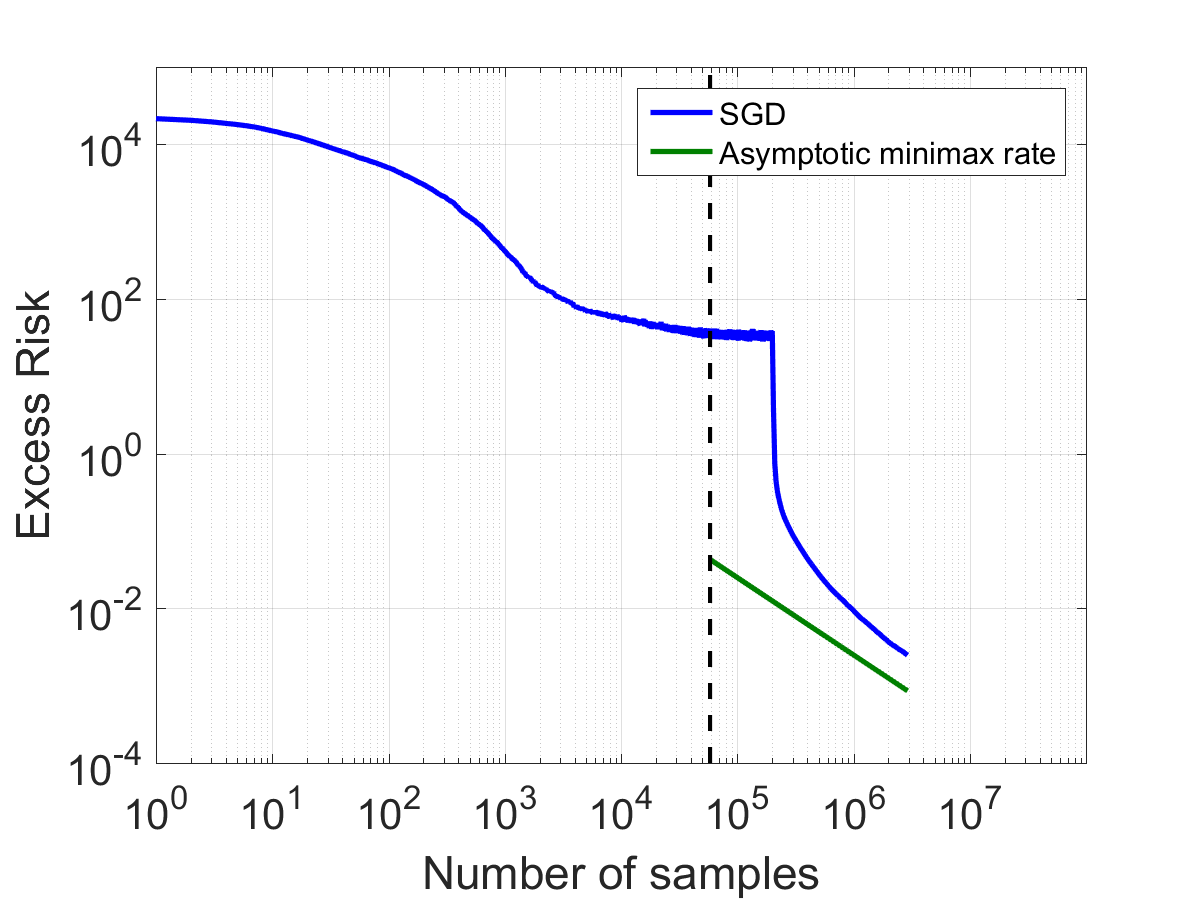
\includegraphics[width=0.49\textwidth]{figures/newer-figs/Multinomial-Total-SGD.png}}
	\subfigure[Gaussian Distribution]{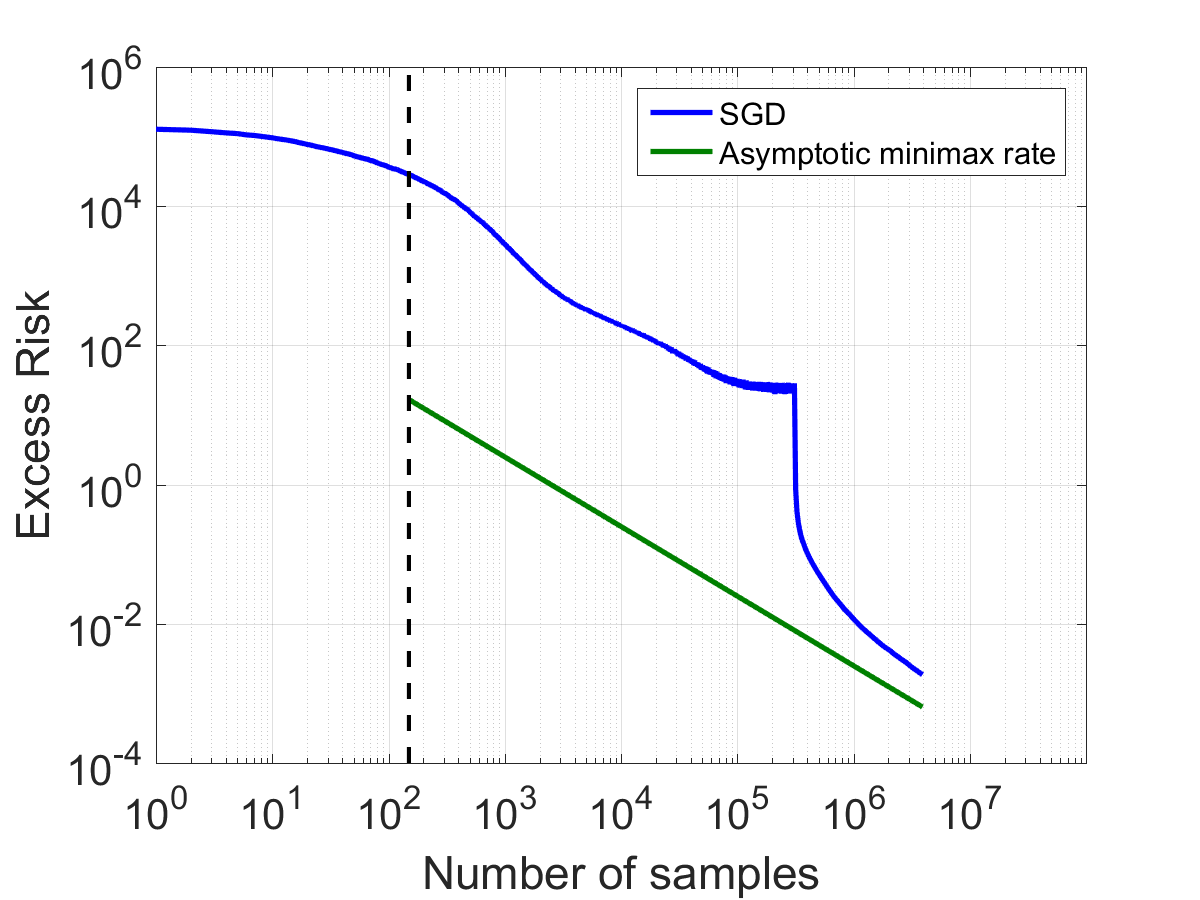
\includegraphics[width=0.49\textwidth]{figures/newer-figs/Gaussian-Total-SGD.png}}
	\vspace*{-2mm}
	\caption{Plot of total error vs number of samples for averaged
          SGD and the minimax risk (green) of $d\sigma^2/n$ for the discrete and
          Gaussian distributions with $d=50$, $\cnH\approx 10^5$ (see section~\ref{sec:exp} for
          details on the distribution). The kink in the SGD curve
          represents when the tail-averaging phase
          begins~\citep{JainKKNS16}; this point is chosen appropriately. The vertical dashed line shows the sample size at which
the empirical covariance, $\frac{1}{n}\sum_{i=1}^n \a_i\a_i\T$,
becomes full rank, which is shown at $\frac{1}{\min_i p_{i}}$ in the
discrete case and $d$ in the Gaussian case. With fewer samples than
this (i.e. before the dashed line), it is information theoretically not possible to guarantee
non-trivial risk (without further assumptions). For the Gaussian case,
note how the behavior of SGD is far from the minimax risk; it is this
behavior that one might hope to improve upon.  See the text for more discussion.
}  \vspace*{-.7cm}
\label{fig:exp} 
\end{figure}
This paper seeks to address the question: ``Can we  accelerate
stochastic approximation in a manner similar to what has been achieved
with the exact first order oracle model?''
\subsection{A thought experiment: Is Accelerating Stochastic Approximation possible?}\label{sec:exp}
Let us recollect known results in stochastic approximation for the least squares regression problem (in equation~\ref{eq:objFun}). Running $n$-steps of tail-averaged SGD~\citep{JainKKNS16} (or, streaming SVRG~\citep{FrostigGKS15}\footnote{Streaming SVRG does not function in the stochastic first order oracle model~\citep{FrostigGKS15}}) provides an output $\xhat_n$ that satisfies the following excess risk bound:
\vspace{-0.3cm}
\begin{align} \label{eq:sgd_rate}
\E{P(\xhat_n)}-P(\xs)\leq \exp(-n/\cnH) \cdot \big(P(\x_0)-P(\xs)\big) + 2\sigma^2d/n,
\end{align}

\vspace{-0.3cm}
\noindent where $\cnH$ is the condition number
of the distribution, which can be upper bounded as $L/\lamminH$,
assuming that $\|\a\|\leq L$ with probability one (refer to
section~\ref{sec:prob} for a precise definition of $\cnH$)\iffalse\footnote{technically,
  averaged SGD~\citep{JainKKNS16} contains a (lower order) factor in
  $d$ in the coefficient of the bias term.}\fi.  Under appropriate
assumptions, these are the best known rates under the stochastic first
order oracle model (see section~\ref{sec:related} for further discussion).
  A natural implication of the bound implied by averaged SGD is that with $\widetilde{\mathcal{O}}(\cnH)$ oracle
calls~\citep{JainKKNS16} (where, $\widetilde{\mathcal{O}}(\cdot)$ hides $\log$ factors in $d,\cnH$), the excess risk attains (up to
constants) the (asymptotic) minimax statistical rate. Note that the excess
risk bounds in stochastic approximation consist of two terms:
(a) {\em bias}: which represents the dependence of the generalization
error on the initial excess risk $P(\x_0)-P(\xs)$, and (b) the {\em
  variance:} which represents the dependence of the generalization
error on the noise level $\sigma^2$ in the problem.

A precise question regarding accelerating stochastic
approximation is: ``is it possible to improve the rate of decay of the
bias term, while retaining (up to constants) the statistical minimax
rate?'' The key technical challenge in answering this question is in
sharply characterizing the error accumulation of fast gradient methods
in the stochastic approximation setting. Common folklore and prior
work suggest otherwise: several efforts have attempted to 
quantify instabilities in the face of statistical or
non-statistical
errors~\citep{Paige71,Proakis74,Polyak87,Greenbaum89,RoyS90,SharmaSB98,dAspremont08,DevolderGN13,DevolderGN14,YuanYS16}.
Refer to section~\ref{sec:related} for a discussion on robustness of acceleration to error accumulation.
\begin{figure}[t]
\centering
	\subfigure[Discrete Distribution]{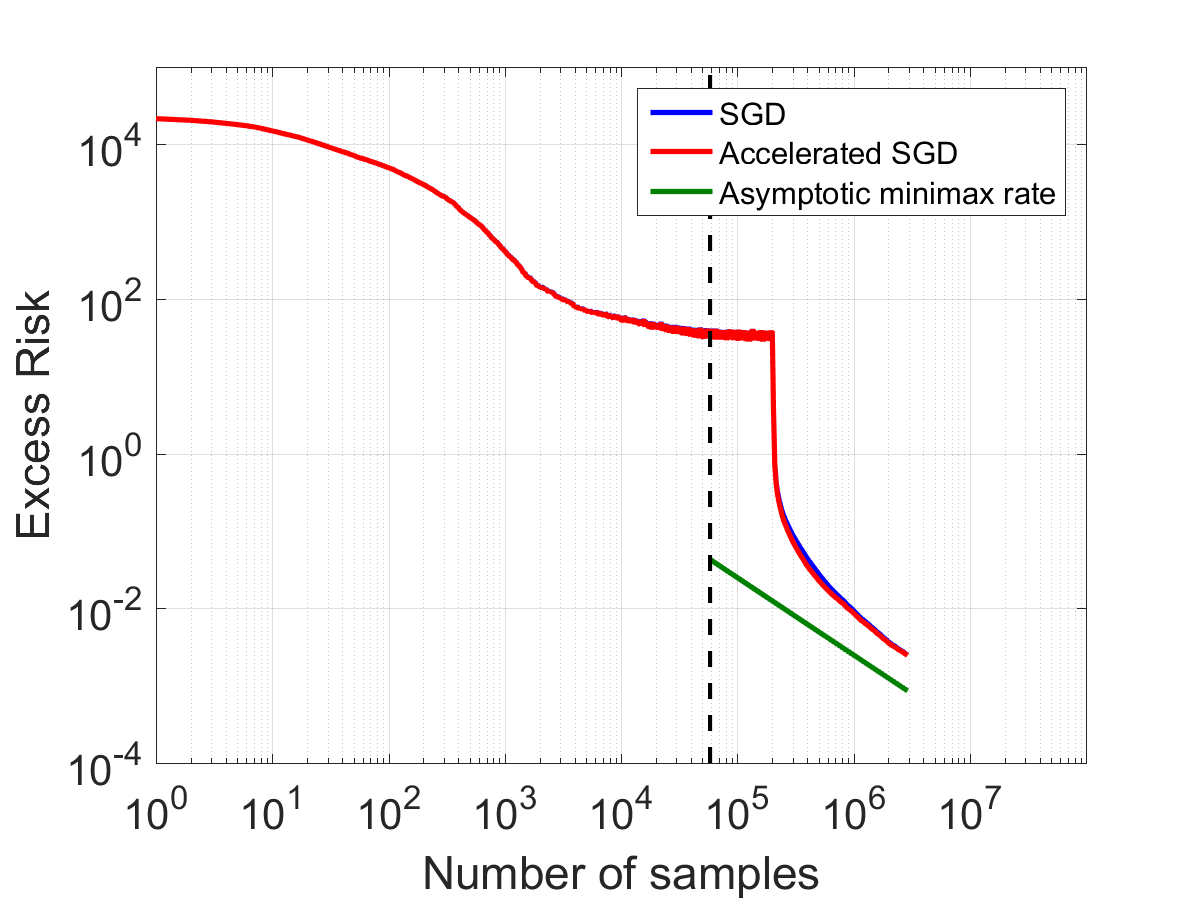
\includegraphics[width=0.49\textwidth]{figures/newer-figs/Multinomial-Total.png}}
	\subfigure[Gaussian Distribution]{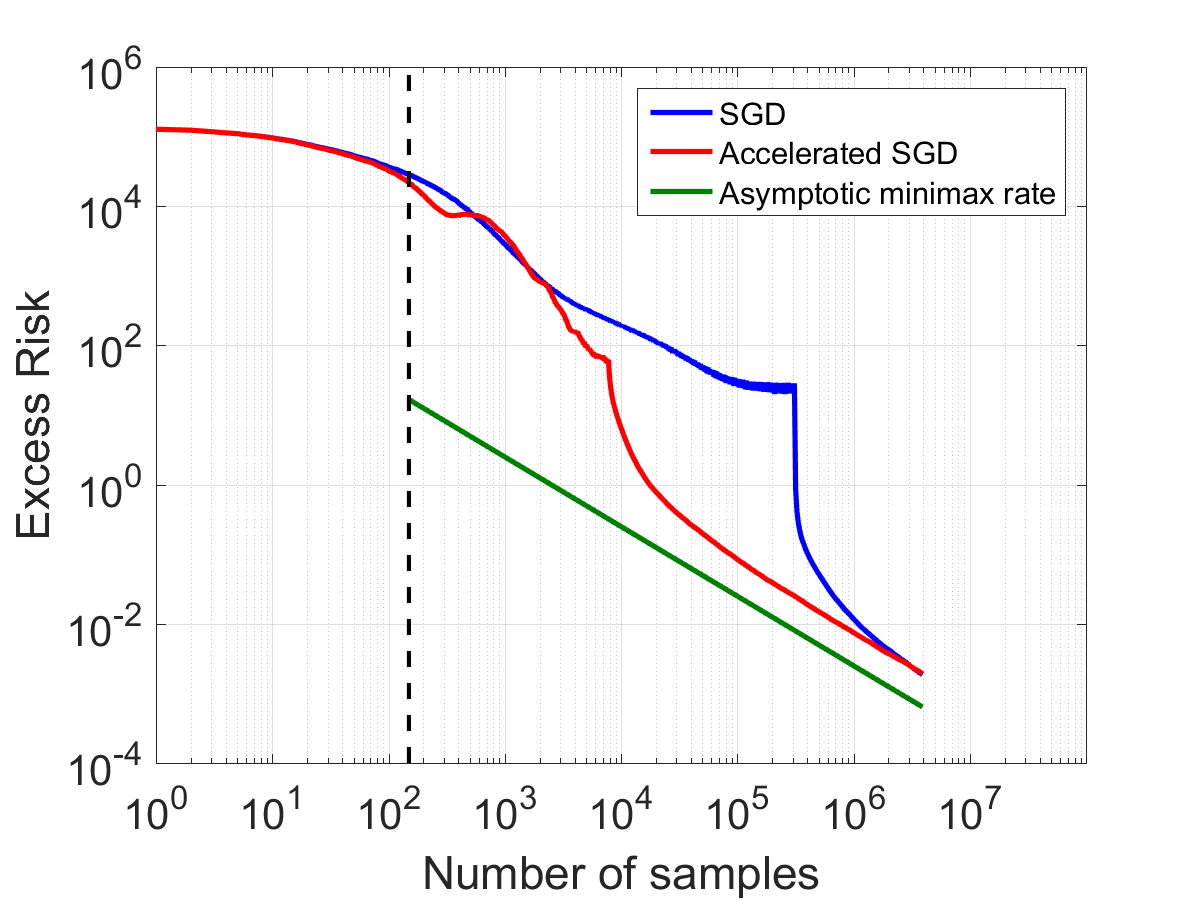
\includegraphics[width=0.49\textwidth]{figures/newer-figs/Gaussian-Total.png}}
	\vspace*{-2mm}
	\caption{Plot of total error vs number of samples for averaged
          SGD, (this paper's) accelerated SGD method and the minimax risk for the discrete and Gaussian distributions with $d=50,\cnH\approx 10^5$ (see section~\ref{sec:exp} for
          details on the distribution). For the discrete case,
          accelerated SGD mimics SGD, which nearly matches the
          minimax risk (when it becomes well defined). For the
          Gaussian case, accelerated SGD significantly improves upon
          SGD. }\vspace*{-0.8cm}\label{fig:res}
\end{figure}
Optimistically, as suggested by the gains enjoyed by accelerated methods in the exact first order oracle model, we may hope to replace the $\widetilde{\mathcal{O}}(\cnH)$ oracle calls achieved by averaged SGD to $\widetilde{\mathcal{O}}(\sqrt{\cnH})$.  We now provide a counter example, showing that such an improvement is not possible. Consider a (discrete) distribution $\D$ where the input $\a$ is the $i^{\textrm{th}}$ standard basis vector with probability $p_i$, $\forall\ i=1,2,...,d$. The covariance of $\a$ in this case is a diagonal matrix with diagonal entries $p_i$. The condition number of this distribution is $\cnH = \frac{1}{\min_i p_{i}}$. In this case, it is impossible to
make non-trivial reduction in error by observing fewer than $\cnH$ samples, since with constant probability, we would not have seen the vector corresponding to the smallest probability. 

On the other hand, consider a case where the distribution $\D$ is a
Gaussian with a large condition number $\cnH$. Matrix concentration
informs us that (with high probability and irrespective of how large $\cnH$ is) after observing
$n=\mathcal{O}(d)$ samples, the empirical covariance matrix will be a spectral approximation to the true covariance
matrix, i.e. for some constant $c>1$,
$\Cov/c \preceq \frac{1}{n}\sum_{i=1}^n \a_i\a_i\T \preceq c \Cov$.
Here, we may hope to achieve a faster convergence rate, as information
theoretically $\mathcal{O}(d)$ samples suffice to obtain a non-trivial
statistical estimate (see~\cite{HsuKZ14} for further discussion).

Figure~\ref{fig:exp} shows the behavior of SGD in these cases;
both are synthetic examples in $50-$dimensions, with a condition
number $\cnH\approx 10^5$ and noise level $\sigma^2=100$. See the figure caption for more details. 

These examples suggest that if acceleration is indeed possible, then the degree of 
improvement (say, over averaged SGD) must depend on distributional 
quantities that go beyond the condition number $\kappa$.
A natural conjecture is that this improvement must depend on 
the number of samples required to spectrally approximate 
the covariance matrix of the distribution; below this sample size it is 
not possible to obtain any non-trivial statistical estimate due 
to information theoretic reasons. This sample size is quantified by a
notion which we refer to as the {\em statistical condition number} $\cnS$ (see
section~\ref{sec:prob} for a precise definition and for further
discussion about $\cnS$). As we will see in section~\ref{sec:prob}, we have $\cnS\leq\cnH$, $\cnS$ is affine invariant, unlike $\cnH$ (i.e. $\cnS$ is invariant to linear transformations over $\a$).\vspace*{-1mm}
\begin{figure}[t]
\centering
	\subfigure[Discrete Distribution]{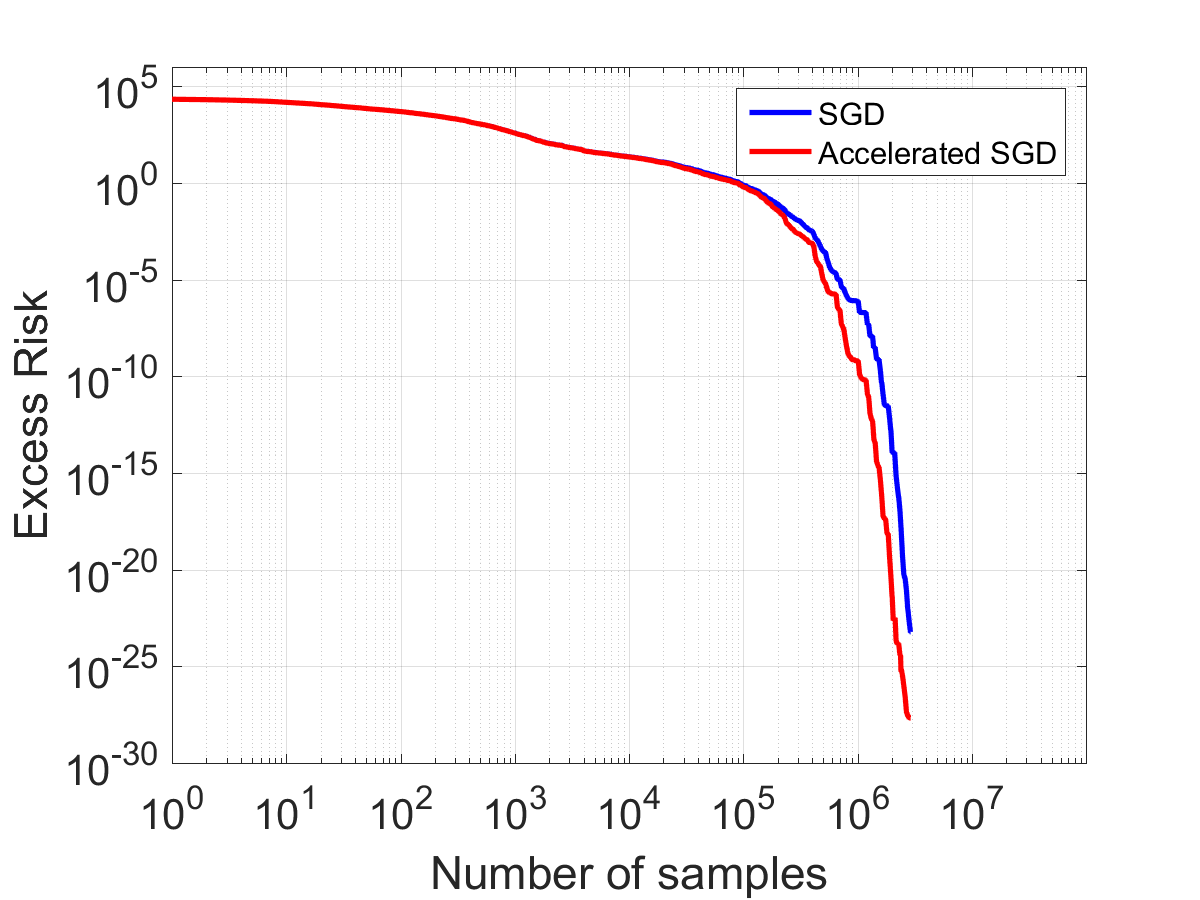
\includegraphics[width=0.49\textwidth]{figures/newer-figs/Multinomial-Bias.png}}
	\subfigure[Gaussian Distribution]{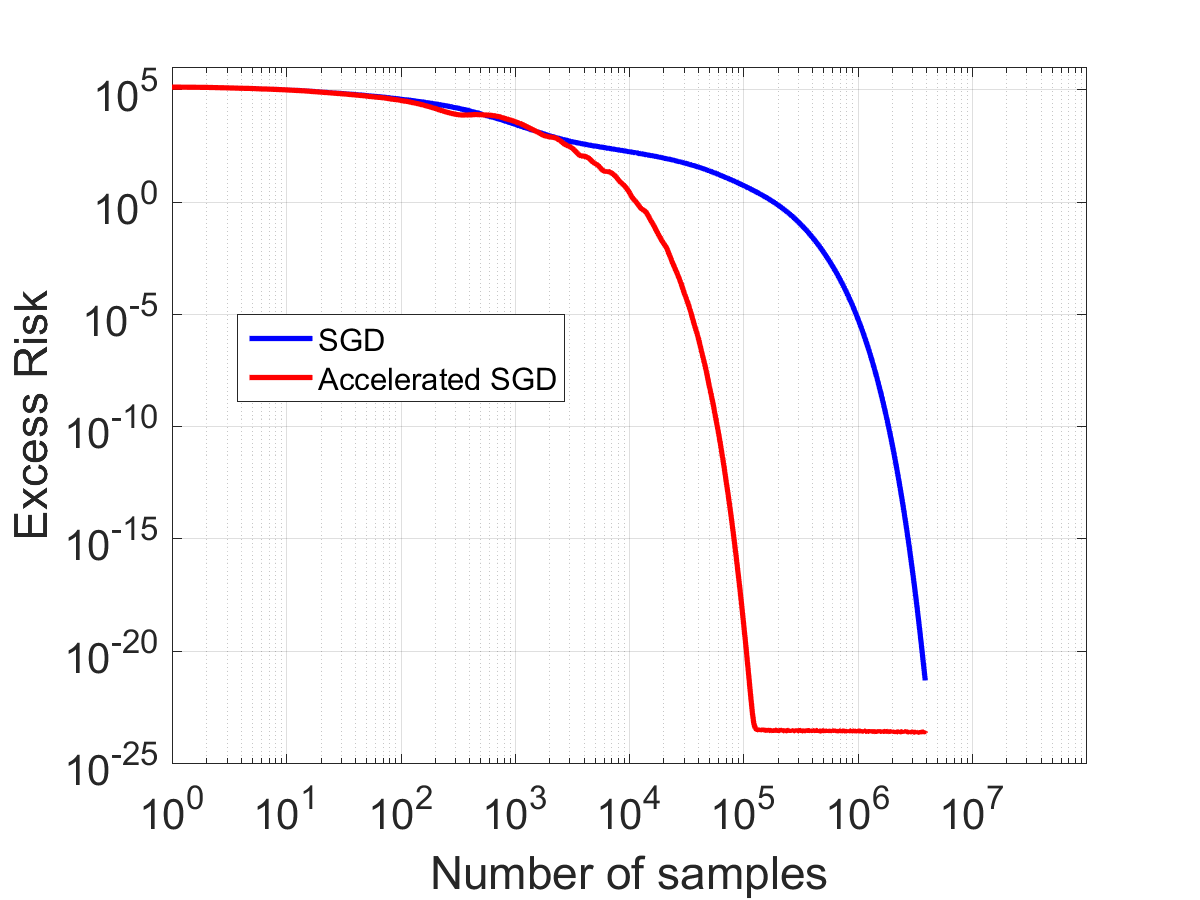
\includegraphics[width=0.49\textwidth]{figures/newer-figs/Gaussian-Bias.png}}
	\vspace*{-2mm}
\caption{Comparison of averaged SGD with this paper's accelerated SGD
  in the absence of noise ($\sigma^2=0$) for the Discrete and Gaussian
  distributions with $d=50,\cnH\approx 10^5$. Acceleration yields
  substantial gains over averaged SGD for the Gaussian case, while
  degenerating to SGD's behavior for the discrete case.
  See section~\ref{sec:exp} for discussion.}\vspace*{-0.8cm}
\label{fig:bias}
\end{figure}
\subsection{Contributions}\label{sec:res}
This paper introduces an accelerated stochastic gradient descent
scheme, which can be viewed as a stochastic variant of Nesterov's accelerated gradient method~\citep{Nesterov12}. As pointed out in Section~\ref{sec:exp}, the excess risk of this algorithm can be decomposed into two parts namely, \emph{bias} and \emph{variance}. For the stochastic approximation problem of least squares regression, this paper establishes bias contraction at a geometric rate of $\mathcal{O}(1/\sqrt{\cnH\cnS})$, improving over prior results~\citep{FrostigGKS15,JainKKNS16},\iffalse (such as averaged SGD~\citep{JainKKNS16}, streaming SVRG~\citep{FrostigGKS15}),\fi which prove a geometric rate of $\mathcal{O}(1/\cnH)$, while retaining statistical minimax rates (up to constants) for the variance. Here $\cnH$ is the condition number and $\cnS$ is the statistical condition number of the distribution, and a rate of $\mathcal{O}(1/\sqrt{\cnH\cnS})$ is an improvement over $\mathcal{O}(1/\cnH)$ since $\cnS \leq \cnH$ (see Section~\ref{sec:prob} for definitions and a short proof of $\cnS \leq \cnH$).

See Table~\ref{tab:comp} for a theoretical comparison. Figure~\ref{fig:res} provides an empirical comparison of the proposed (tail-averaged) accelerated algorithm to (tail-averaged) SGD~\citep{JainKKNS16} on our two running examples. Our result gives improvement over SGD even in the noiseless (i.e. realizable) case where $\sigma=0$; this case is equivalent to the setting where we have a distribution over a (possibly infinite) set of consistent linear equations. See Figure~\ref{fig:bias} for a comparison
on the case where $\sigma=0$.


On a more technical note, this paper introduces two new techniques in
order to analyze the proposed accelerated stochastic gradient method:
(a) the paper introduces a new potential function in order to
show faster rates of decaying the bias, and (b) the paper
provides a sharp understanding of the behavior of the
proposed accelerated stochastic gradient descent updates as a
stochastic process and utilizes this in providing a near-exact
estimate of the covariance of its iterates. This
viewpoint is critical in order to prove that the algorithm
achieves the statistical minimax rate. 

We use the operator viewpoint for analyzing stochastic
gradient methods, introduced in~\cite{DefossezB15}. This
viewpoint was also used in~\cite{DieuleveutB15,JainKKNS16}.


\subsection{Related Work}
\label{sec:related}
\paragraph{Non-asymptotic Stochastic Approximation:} Stochastic gradient descent (SGD) and its variants are by far the most
widely studied algorithms for the stochastic approximation problem.
While initial works~\citep{RobbinsM51} considered the final iterate of
SGD, later works~\citep{Ruppert88,PolyakJ92} demonstrated that averaged
SGD obtains statistically optimal estimation rates. Several 
works provide non-asymptotic analyses for averaged
SGD and variants~\citep{BachM11,Bach14,FrostigGKS15} for various
stochastic approximation problems. For stochastic approximation with
least squares regression~\citet{BachM13,DefossezB15,NeedellSW16,FrostigGKS15,JainKKNS16}
provide non-asymptotic analysis of the behavior of SGD and its
variants. \cite{DefossezB15,DieuleveutB15} provide non-asymptotic results which achieve the minimax rate on the variance (where the bias is lower order, not geometric).
\cite{NeedellSW16} achieves a geometric rate on the bias (and where the variance is not minimax). \cite{FrostigGKS15,JainKKNS16} obtain both the minimax rate on the variance and a geometric rate on the bias, as seen in equation~\ref{eq:sgd_rate}. 

\iffalse
 The works in \cite{BachM13,DefossezB15} achieve the minimax
rate on the variance, while \cite{NeedellSW16} achieves a geometric
rate of decay on the bias; \cite{FrostigGKS15,JainKKNS16} obtain both
the minimax rate on the variance and a geometric rate of decay on the
bias, as seen in equation~\ref{eq:sgd_rate}. 
\fi

%\rahul{write about \cite{DevolderGN13,Devolder13} as well.}
\paragraph{Acceleration and Noise Stability:}  
While there have been several attempts at understanding if it is
possible to accelerate SGD , the results have been largely negative.
With regards to acceleration with adversarial (non-statistical) errors in the exact first order oracle model,~\cite{dAspremont08} provide negative results and \citet{DevolderGN13,DevolderGN14} provide
lower bounds showing that fast gradient methods do not improve upon
standard gradient methods. There is also a series of works considering
statistical errors.~\cite{Polyak87} suggests that the relative
merits of heavy ball (HB) method~\citep{Polyak64} in the noiseless case
vanish with noise unless strong assumptions on the
noise model are considered; an instance of this is when the
noise variance decays as the iterates approach the minimizer. The
Conjugate Gradient (CG) method~\citep{HestenesS52} is suggested to face
similar robustness issues in the face of statistical
errors~\citep{Polyak87}; this is in addition to the issues that CG is
known to suffer from owing to roundoff errors (due to finite precision
arithmetic)~\citep{Paige71,Greenbaum89}. In the signal processing
literature, where SGD goes by Least Mean Squares
(LMS)~\citep{WidrowS85}, there have been efforts that date to several
decades~\citep{Proakis74,RoyS90,SharmaSB98} which study accelerated LMS
methods (stochastic variants of CG/HB) in the
same oracle model as the one considered by this paper
(equation~\ref{eq:stochFirstOrderOracle}). These efforts consider the
final iterate (i.e. no iterate averaging) of accelerated LMS
methods with a fixed step-size and conclude that while it allows for a
faster decay of the initial error (bias) (which is unquantified), their steady state behavior (i.e. variance) is worse
compared to that of LMS. \citet{YuanYS16} considered a
constant step size accelerated scheme with no iterate averaging in the same oracle model as this paper, and conclude that these do not offer any improvement over standard SGD. More concretely, \citet{YuanYS16} show that the
variance of their accelerated SGD method with a sufficiently small constant step size is the same as that of SGD with a significantly larger step size. Note that none of the these efforts~\citep{Proakis74,RoyS90,SharmaSB98,YuanYS16} achieve minimax
error rates or quantify (any improvement whatsoever on the) rate of bias decay.

\paragraph{Oracle models and optimality:}With regards to notions of optimality, there are (at least) two lines
of thought: one is a statistical objective where the goal is (on every
problem instance) to match the rate of the statistically optimal
estimator~
\citep{anbar1971optimal,Fabian:1973:AES,KushnerClark,PolyakJ92};
another is on obtaining algorithms whose worst case upper bounds
(under various assumptions such as bounded noise) match the lower
bounds provided in ~\cite{NemirovskyY83}.  The work of~\cite{PolyakJ92} are in the former model, where
they show that the distribution of the averaged SGD
estimator matches, on \emph{every} problem, that of the statistically
optimal estimator, in the limit (under appropriate regularization
conditions standard in the statistics literature, where the optimal
estimator is often referred to as the maximum likelihood estimator/the
empirical risk minimizer/an
$M$-estimator~\citep{lehmann1998theory,Vaart00}). Along these lines,
non-asymptotic rates towards statistically optimal estimators are
given
by~\cite{BachM13,Bach14,DefossezB15,DieuleveutB15,NeedellSW16,FrostigGKS15,JainKKNS16}. This work can be seen as improving this non-asymptotic rate (to the
statistically optimal estimation rate) using an accelerated method. As to the latter (i.e. matching the worst-case lower bounds in
~\cite{NemirovskyY83}), there are a number of 
positive results on using accelerated stochastic
optimization procedures; the works
of~\cite{Lan08,HuKP09,ghadimi2012optimal,ghadimi2013optimal,DieuleveutFB16}
match the lower bounds provided in~\cite{NemirovskyY83}. We
compare these assumptions and works in more detail.

In stochastic first order oracle models (see ~\cite{KushnerClark,KushnerY03}), one typically has access to sampled gradients of the form:%\vspace*{-1mm}
\vspace{-0.2cm}
\begin{align}
\widehat{\nabla}P(\x)  = \nabla P(\x) + \etav, \label{eq:stochFirstOrderOracle-diff}
\end{align}

\vspace{-0.2cm}
\noindent where varying assumptions are made on the noise $\etav$. The
worst-case lower bounds in~\cite{NemirovskyY83} are based
on that $\etav$ is bounded; the accelerated methods in~\citet{Lan08,HuKP09,ghadimi2012optimal,ghadimi2013optimal,DieuleveutFB16}
which match these lower bounds in various cases, all assume either
bounded noise or, at least $\E{\|\etav\|^2}$ is finite. In
the least squares setting (such as the one often considered in
practice and also considered in~\citet{PolyakJ92,BachM13,DefossezB15,DieuleveutB15,FrostigGKS15,JainKKNS16}),
this assumption does not hold, since $\E{\|\etav\|^2}$ is
not bounded. To see this, $\etav$ in our oracle model (equation~\ref{eq:stochFirstOrderOracle}) is:
%in our oracle model (equation~\ref{eq:stochFirstOrderOracle}), $\etav$ can be written as:
\vspace{-0.2cm}
\begin{align}
  \label{eq:noiseModel2}
\etav=\widehat{\nabla}P(\x)-\nabla P(\x)=(\a\a\T-\Cov)(\x-\xs)-\epsilon\cdot\a
\end{align}

\vspace{-0.2cm}
\noindent which implies that $\E{\|\etav\|^2}$ is not uniformly bounded (unless
additional assumptions are enforced to ensure that the algorithm's
iterates $\x$ lie within a compact set).  Hence, the assumptions made
in~\cite{HuKP09,ghadimi2012optimal,ghadimi2013optimal,DieuleveutFB16}
do not permit one to obtain finite $n$-sample bounds on the excess
risk.  Suppose we consider the case of $\epsilon=0$, i.e. where the
additive noise is zero and $\b=\a \T \xs$.  For this case, this
paper provides a geometric rate of convergence to the minimizer $\xs$,
while the results of~\cite{ghadimi2012optimal,ghadimi2013optimal,DieuleveutFB16}
at best indicate a $\mathcal{O}(1/n)$ rate. Finally, in contrast to all other existing work, our result is the first to provide finer distribution dependent characteristics of the improvements offered by accelerating SGD (e.g.  refer to the Gaussian and discrete examples in section~\ref{sec:exp}).

\paragraph{Acceleration and Finite Sums:} As a final remark, there have been
results~\citep{ShwartzZ14,FrostigGKS15b,LinMH15,LanZ15,Zhu16} that provide accelerated
rates for {\em offline} stochastic optimization which deal with
minimizing sums of convex functions; these results are almost
tight due to matching lower bounds~\citep{LanZ15,WoodworthS16}. These
results do not immediately translate into rates on the generalization
error.
%In order to convert these statements to generalization error bounds, these results require going through concentration of the ERM as well as a generalization error analysis. 
Furthermore, these algorithms are not streaming, as they require making multiple passes over a
dataset stored in memory. Refer to~\citet{FrostigGKS15} for more details.\vspace*{-2mm}



\section{Main Results}
\label{sec:prob}
%This work considers the stochastic approximation problem in equation~\eqref{eq:objFun}. 
%Given access to a stochastic first order oracle (equation~\eqref{eq:stochFirstOrderOracle}), the goal is
%to design a streaming algorithm that minimizes $P(\x)$ at near to the statistically optimal rate.

We now provide our assumptions and main result, before which, we have some notation. For a vector $\x\in\R^d$ and a positive semi-definite matrix $\S\in\R^{d\times d}$ (i.e. $\S\succeq0$), denote $\|\x\|^2_\S \eqdef  \x\T \S \x$.\vspace*{-2mm}
\subsection{Assumptions and Definitions}
Let $\Cov$ denote the second moment matrix of the input, which is also the hessian $\nabla^2P(\x)$ of~\eqref{eq:objFun}:%\vspace*{-1mm}
\vspace{-0.2cm}
\begin{align*}
\Cov \eqdef \Eover{\distr}{\a\otimes\a} = \nabla^2P(\x).
\end{align*}
%Assume:
\vspace{-.8cm}
\begin{enumerate}[leftmargin=*,label=$\mathbf{(\mathcal A\arabic*)}$]
\item \label{asmp:finiteness} \textbf{Finite second and fourth moment:} The second moment matrix $\H$ and the fourth moment tensor $\M\ (=\Eover{\distr}{\a\otimes\a\otimes\a\otimes\a})$ of the input $\a\sim\D$ exist and are finite.
\item \label{asmp:positiveDefinite}\textbf{Positive Definiteness}: The second moment matrix $\Cov$ is strictly positive definite, i.e. $\Cov\succ0$.
\end{enumerate}
%Assumption~\ref{asmp:finiteness}and~\ref{asmp:positiveDefinite} are common in stochastic approximation for the purpose of proving non-asymptotic rates, see for example~\cite{KushnerY03,BachM11,DefossezB15,FrostigGKS15}.

\noindent We assume~\ref{asmp:finiteness} and~\ref{asmp:positiveDefinite}.~\ref{asmp:positiveDefinite} implies that $P(\x)$
is {\em strongly convex} and admits a unique minimizer
$\xs$. Denote the noise $\epsilon$ in a sample $(\a,b)\sim\D$ as: $\n \eqdef \b - \iprod{\a}{\xs}$. First order optimality conditions of $\xs$ imply $\nabla P(\xs) = \E{\n \cdot \a} = 0$.
Let $\Sig$ denote the covariance of gradient at optimum $\xs$ (or {\em noise covariance matrix}), $\Sig \defeq\Eover{\distr}{\widehat{\nabla}P(\xs)\otimes\widehat{\nabla}P(\xs)}=\Eover{\distr}{\n^2\cdot\a\otimes\a}$.

\noindent We define the \emph{noise level} $\sigma^2$, \emph{condition number} $\cnH$, \emph{statistical condition number} $\cnS$ below.\\
\noindent\textbf{Noise level}: The \emph{noise level} is defined to be the smallest positive number $\sigma^2$ such that $\Sig\preceq \sigma^2\H$.\iffalse\vspace*{-2mm}
\begin{align*}
\Sig\preceq\sigma^2\ \Cov.
\end{align*}\fi
The noise level $\sigma^2$ quantifies the amount of noise in the
stochastic gradient oracle and has been utilized in previous work (e.g., see~\cite{BachM11,BachM13}) in providing non-asymptotic bounds for the stochastic approximation problem. In the \emph{homoscedastic} (additive noise) case, where $\n$ is independent of the input $\a$, this condition is satisfied with equality, i.e. $\Sig = \sigma^2\ \Cov$ with $\sigma^2 = \E{\epsilon^2}$.\\
\noindent\textbf{Condition number}: Let $\mu\defeq\lamminH$. $\mu>0$ by \ref{asmp:positiveDefinite}. Now, let $\infbound$ be the smallest positive number such that $\E{\|\a\|^2\ \a\a\T} \preceq \infbound\ \Cov$. The \emph{condition number} $\cnH$ of the distribution $\D$~\citep{DefossezB15,JainKKNS16} is $
\cnH \defeq {\infbound}/{\mu}$.

\noindent \textbf{Statistical condition number}: The \emph{statistical condition number} $\cnS$ is defined as the smallest positive number such that $\E{\Hinvnorm{\a}^2\a\a\T}\preceq \cnS\ \Cov$. 
%\E{(\a\T\H\inv\a)\a\a\T}\preceq \cnS\ \Cov. 

\noindent\textbf{Remarks on $\cnS$ and $\cnH$}:
Unlike $\cnH$, it is straightforward to see that $\cnS$ is affine invariant 
(i.e. unchanged with linear transformations over $\a$). 
Since $\E{\Hinvnorm{\a}^2\a\a\T}\preceq \frac{1}{\mu}
\E{\twonorm{\a}^2\a\a\T}\preceq \cnH \Cov$, we note $\cnS \leq \cnH$. For the discrete case
(from Section~\ref{sec:exp}), it is straightforward
to see that both $\cnH$ and $\cnS$ are equal to $1/\min_i p_{i}$. In
contrast, for the Gaussian case (from Section~\ref{sec:exp}), $\cnS$
 is $\mathcal{O}(d)$, while $\cnH$ is
 $\mathcal{O}(\textrm{Trace}(\Cov)/\mu)$ which may be arbitrarily large (based on
 choice of the coordinate system).

$\cnS$ governs how many samples $\ai$ require to be drawn from $\D$ so
 that the empirical covariance is spectrally close to $\Cov$,
 i.e. for some constant $c>1$, $\Cov/c \preceq \frac{1}{n}\sum_{i=1}^n \a_i\a_i\T \preceq c \Cov$.
 In comparison to the matrix Bernstein inequality where stronger (yet related) moment
 conditions are assumed in order to obtain high probability results,
 our results hold only in expectation (refer to~\citet{HsuKZ14} for this definition, wherein $\cnS$ is referred to as bounded statistical leverage in theorem $1$ and remark $1$).\vspace*{-2mm}

\iffalse
\begin{algorithm}[t]
	\caption{ (Tail-Averaged) \textbf{A}ccelerated \textbf{S}tochastic \textbf{G}radient
          \textbf{D}escent (ASGD)}
	\label{algo:TAASGD}
	\begin{algorithmic}[1]
		\INPUT $n$ oracle calls~\ref{eq:stochFirstOrderOracle}, initial point $\xt[0]=\vt[0]$, Unaveraged (burn-in) phase $t$, Step size parameters $\alpha, \beta, \gamma, \delta$
		\FOR{$j = 1, \cdots n$}
		\STATE $\yt[j-1] \leftarrow \alpha \xt[j-1] + (1-\alpha) \vt[j-1]$
		\STATE $\xt[j] \leftarrow \yt[j-1] - \delta \widehat{\nabla} P(\yt[j-1])$
		\STATE $\zt[j-1] \leftarrow \beta \yt[j-1] + (1-\beta) \vt[j-1]$
		\STATE $\vt[j] \leftarrow \zt[j-1] - \gamma \widehat{\nabla} P(\yt[j-1])$
		\ENDFOR
		\OUTPUT $\bar{\x}_{t,n} \leftarrow \frac{1}{n-t}\sum_{j=t+1}^{n} \xt[j]$
	\end{algorithmic}
\end{algorithm}
\fi
%\dontprintsemicolon
%\LinesNumbered
%\RestyleAlgo{boxruled}
%\restylealgo{boxed}
%\RestyleAlgo{boxruled}
%\LinesNumbered
%\RestyleAlgo{boxed}
%\LinesNumbered
\begin{algorithm}[t]
	\caption{(Tail-Averaged) \textbf{A}ccelerated \textbf{S}tochastic \textbf{G}radient
          \textbf{D}escent (ASGD)}
		\KwIn{$n$ oracle calls to~\ref{eq:stochFirstOrderOracle}, initial iterate $\xt[0]=\vt[0]$, Unaveraged (burn-in) phase $t$, Step sizes $\alpha, \beta, \gamma, \delta$}
		\KwOut{$\bar{\x}_{t,n} \leftarrow \frac{1}{n-t}\sum_{j=t+1}^{n} \xt[j]$}
		\For{$j \gets 1$ \KwTo $n$}{
		$\ \ \yt[j-1] \leftarrow \alpha \xt[j-1] + (1-\alpha) \vt[j-1]$\;\\
		$\xt[j] \leftarrow \yt[j-1] - \delta \widehat{\nabla} P(\yt[j-1])$\;\\
		$\zt[j-1] \leftarrow \beta \yt[j-1] + (1-\beta) \vt[j-1]$\;\\
		$\vt[j] \leftarrow \zt[j-1] - \gamma \widehat{\nabla} P(\yt[j-1])$\;
		}
	\label{algo:TAASGD}
\end{algorithm}
\subsection{Algorithm and Main Theorem}\label{sec:results}%\label{sec:algo}
Algorithm~\ref{algo:TAASGD} presents the pseudo code of the proposed algorithm. ASGD can be viewed as a variant of Nesterov's accelerated gradient method~\citep{Nesterov12}, working with a stochastic gradient oracle (equation~\ref{eq:stochFirstOrderOracle}) and with tail-averaging the final $n-t$ iterates. The main result now follows:%\vspace*{-6mm}
\begin{theorem}\label{thm:main}
Suppose ~\ref{asmp:finiteness} and
~\ref{asmp:positiveDefinite} hold. Set $\alpha =
\frac{3\sqrt{5}\cdot\sqrt{\cnH\cnS}}{1+3\sqrt{5}\cdot\sqrt{\cnH\cnS}},
\beta = \frac{1}{9\sqrt{\cnH\cnS}}, \gamma =  \frac{1}{3\sqrt{5}\cdot
  \mu \sqrt{\cnH\cnS}}, \delta = \frac{1}{5R^2}$. After $n$ calls to
the stochastic first order oracle
(equation~\ref{eq:stochFirstOrderOracle}), ASGD
outputs $\bar{\x}_{t,n}$ satisfying:
% the following excess risk guarantee:
\vspace{-0.3cm}
\iffalse
	\begin{align*}
	&\E{P(\bar{\x}_{t,n})}-P(\xs) \leq \underbrace{\UC\cdot\frac{(\cnH\cnS)^{9/4}d\cnH}{(n-t)^2}\cdot\exp\bigg(\frac{-t}{9\sqrt{\cnH\cnS}}\bigg)\cdot\big(P(\x_0)-P(\xs)\big)}_{\text{Leading order bias error}}+\underbrace{5\frac{\sigma^2d}{n-t}}_{\text{Leading order variance error}} + \nonumber\\&\underbrace{\UC\cdot(\cnH\cnS)^{5/4}d\cnH\cdot\exp\left(\frac{-n }{9\sqrt{\cnH\cnS}}\right) \big(P(\x_0)-P(\xs)\big)}_{\text{Exponentially vanishing lower order bias term}} + \underbrace{\UC\cdot\frac{\sigma^2 d}{(n-t)^2} \sqrt{\cnH\cnS}}_{\text{Lower order variance error term}}+\nonumber\\ &{\small \underbrace{\UC\cdot\bigg(\sigma^2d\cdot(\cnH\cnS)^{7/4}\cdot\exp\bigg(\frac{-n}{9\sqrt{\cnH\cnS}}\bigg)+\frac{\sigma^2d}{n-t}(\cnH\cnS)^{11/4}\exp\bigg({-\frac{(n-t-1)}{30\sqrt{\cnH\cnS}}}\bigg) +\frac{\sigma^2d}{(n-t)^2}\cdot\exp\bigg({-\frac{n}{9\sqrt{\cnH\cnS}}}\bigg)\cdot(\cnH\cnS)^{7/2}\cnS\bigg)}_{\text{Exponentially vanishing lower order variance error terms}}},%\alpha^{(n-t-1)/2}
	\end{align*}
\fi
	\begin{align*}
	&\E{P(\bar{\x}_{t,n})}-P(\xs) \leq \underbrace{\UC\cdot\frac{(\cnH\cnS)^{9/4}d\cnH}{(n-t)^2}\cdot\exp\bigg(\frac{-t}{9\sqrt{\cnH\cnS}}\bigg)\cdot\big(P(\x_0)-P(\xs)\big)}_{\text{Leading order bias error}}+\underbrace{5\frac{\sigma^2d}{n-t}}_{\text{Leading order variance error}} + \nonumber\\&\underbrace{\UC\cdot(\cnH\cnS)^{5/4}d\cnH\cdot\exp\left(\frac{-n }{9\sqrt{\cnH\cnS}}\right) \big(P(\x_0)-P(\xs)\big)}_{\text{Exponentially vanishing lower order bias term}} + \underbrace{\UC\cdot\frac{\sigma^2 d}{(n-t)^2} \sqrt{\cnH\cnS}}_{\text{Lower order variance error term}}+\nonumber\\ &{\small \underbrace{\UC\cdot\exp\bigg({-\frac{n}{9\sqrt{\cnH\cnS}}}\bigg)\cdot\bigg(\sigma^2d\cdot(\cnH\cnS)^{7/4}+\frac{\sigma^2d}{(n-t)^2}\cdot(\cnH\cnS)^{7/2}\cnS\bigg)+C\cdot\frac{\sigma^2d}{n-t}(\cnH\cnS)^{11/4}\exp\bigg({-\frac{(n-t-1)}{30\sqrt{\cnH\cnS}}}\bigg)}_{\text{Exponentially vanishing lower order variance error terms}}},%\alpha^{(n-t-1)/2}
	\end{align*}

	\vspace{-0.3cm}
	\noindent 
	where $\UC$ is a universal constant, $\sigma^2$, $\cnH$ and $\cnS$ are the noise level, condition number and statistical condition number respectively.
\end{theorem}
The following corollary holds if the iterates are tail-averaged over the last $n/2$ samples and $n>\mathcal{O}(\sqrt{\cnH\cnS}\log(d\cnH\cnS))$. The second condition lets us absorb lower order terms into leading order terms. 
\begin{corollary}\label{cor:lowerOrder}
Assume the parameter settings of theorem~\ref{thm:main} and
let $t=\lfloor n/2 \rfloor$ and $n>\UC'\sqrt{\cnH\cnS}\log(d\cnH\cnS)$ (for
an appropriate universal constants $\UC,\UC'$).
We have that with $n$ calls to the stochastic first order oracle,
ASGD outputs a vector $\bar{\x}_{t,n}$
satisfying:\vspace*{-2mm}
% the following excess risk guarantee:
	\begin{align*}
	&\E{P(\bar{\x}_{t,n})}-P(\xs) \leq \UC \cdot\exp\bigg(-\frac{n}{20\sqrt{\cnH\cnS}}\bigg)\cdot\big(P(\x_0)-P(\xs)\big)+11\frac{\sigma^2d}{n}.
	\end{align*}
%	\vspace*{-2mm}where $\UC$ is a universal constant.
\end{corollary}

A few remarks about the result of theorem~\ref{thm:main} are due: (i) ASGD decays the initial error at a geometric rate of $\mathcal{O}(1/\sqrt{\cnH\cnS})$ during the unaveraged phase of $t$ iterations, which presents the first improvement over the $\mathcal{O}\left(1/\cnH\right)$ rate offered by SGD~\citep{RobbinsM51}/averaged SGD~\citep{PolyakJ92,JainKKNS16} for the least squares stochastic approximation problem, (ii) the second term in the error bound indicates that ASGD obtains (up to constants) the minimax rate once $n>\mathcal{O}(\sqrt{\cnH\cnS}\log(d\cnH\cnS))$. Note that this implies that Theorem~\ref{thm:main} provides a sharp non-asymptotic analysis (up to $\log$ factors) of the behavior of Algorithm~\ref{algo:TAASGD}.\iffalse (iii) as long as the number of burn-in iterations $t$ and the tail-averaged iterations $n-t$ exceed $\mathcal{O}\left(\sqrt{\cnH\cnS}\cdot\log(d\cnH\cnS) \cdot \log \frac{P(\xt[0])-P(\xs)}{(\sigma^2 d)/n}\right)$, algorithm~\ref{algo:TAASGD} achieves (up to constants) the statistically optimal estimation rates, i.e.:
\begin{align*}
&\E{P(\bar{\x}_{t,n})}-P(\xs) \leq C\ \frac{\sigma^2d}{n},
\end{align*}
where $C$ is a universal constant. This implies that the result in theorem~\ref{thm:main} presents a sharp non-asymptotic analysis (up to $\log$ factors) of the behavior of ASGD.\fi%, and obtains the {\em first} improvement over the rates offered by averaged SGD~\cite{JainKKNS16} and streaming SVRG~\cite{FrostigGKS15} for the stochastic approximation problem.



\subsection{Discussion and Open Problems}\label{sec:resultDiscussion}

%\sidford{I would maybe put this after the Proof outline, but I do not have a strong preference.}
A challenging problem in this context is in formalizing a finite sample size lower bound in the oracle model considered in this work.  Lower bounds in stochastic oracle models have been considered in the literature (see~\cite{NemirovskyY83,RaginskyR11,AgarwalBRW12}), though it is not evident these oracle models and lower bounds are sharp enough to imply statements in our setting (see section~\ref{sec:related} for a discussion of these oracle models).

Let us now understand theorem~\ref{thm:main} in the broader context of stochastic approximation. Under certain regularity conditions, it is known that~\citep{lehmann1998theory,Vaart00} that the rate described in equation~\ref{eq:ERMVarianceAdditive} for the homoscedastic case holds for a broader set of misspecified models (i.e., heteroscedastic noise case), with an appropriate definition of the noise variance. By defining $\sigma^2_{\textrm{ERM}}\eqdef\E{\norm{\widehat{\nabla}P(\xs)}^2_{\inv{\H}}}$, the rate of the ERM is guaranteed to approach $\sigma^2_{\textrm{ERM}}/n$~\citep{lehmann1998theory,Vaart00} in the limit of large $n$, i.e.:\vspace*{-2mm} 
\begin{align}
\label{eq:ERMVariance}
	\lim_{n\to\infty}\frac{\mathbb{E}_{\ST_n}[P_n(\xhat_n^{\textrm{ERM}})]-P(\xs)}{\sigma^2_{\textrm{ERM}}/n} &= 1,
\end{align}

\vspace{-0.2cm}
\noindent where $\xhat_n^{\textrm{ERM}}$ is the ERM over samples $\ST_n=\{\a_i,b_i\}_{i=1}^n$. Averaged SGD~\citep{JainKKNS16} and streaming SVRG~\citep{FrostigGKS15} are known to achieve these rates for the heteroscedastic case. \iffalse Refer to~\cite{FrostigGKS15} for more details.\fi Neglecting constants, Theorem~\ref{thm:main} is guaranteed to achieve the rate of the ERM for the {\em homoscedastic} case (where $\Sig=\sigma^2\H$) and is tight when the bound $\Sig\preceq\sigma^2\H$ is nearly tight (upto constants). We conjecture ASGD achieves the rate of the ERM in the heteroscedastic case by appealing to a more refined analysis as is the case for averaged SGD (see~\cite{JainKKNS16}). It is also an open question to understand acceleration for smooth stochastic approximation (beyond least squares), in situations where the rate represented by equation~\ref{eq:ERMVariance} holds~\citep{PolyakJ92}.
\vspace{-3mm}
\iffalse
Other questions include simplifying the analysis of the proposed algorithm. It is also an important open question to understand the behavior of acceleration for smooth stochastic approximation problems going beyond least squares regression, where the rate represented by equation~\ref{eq:ERMVariance} holds.\fi

%\section{Results}
\iffalse
We can combine the above result and observations with the ideas of~\cite{JainKKNS16} to design a mini-batching, tail-averaging, accelerated SGD algorithm that is highly parallelizable. The pseudocode of this algorithm is presented in Algorithm~\ref{algo:PASGD}, which uses the mini-batched version of Algorithm~\ref{algo:TAASGD} i.e., Algorithm~\ref{algo:MBTAASGD}. Algorithm~\ref{algo:PASGD} consists of three phases: i) initial phase, where the bias is decreased to the same level as noise, ii) middle phase, where doubling mini-batch sizes are used for parallelizability and to decrease variance, and iii) final phase, where tail-averaging is used to improve the variance further. Combining Theorem~\ref{thm:main} with the ideas of~\cite{JainKKNS16}, we obtain the following theorem.
\begin{theorem}\label{thm:par}
	Given $n$ samples $(\ai[1],\bi[1]),\cdots, (\ai[n],\bi[n])$ sampled from a distribution $\D(\R^{d}\times \R)$, Algorithm~\ref{algo:PASGD} run with initial mini-batch size $m=\max\left(\frac{R^2}{\twonorm{\Cov}},{\cnS}\right)$, inner loops $q = \sqrt{\kappa(\Cov)} \log \sqrt{d \kappa(\Cov)}$ and parameters $\alpha = \frac{4\sqrt{\kappa(\Cov)}}{\sqrt{7}+4\sqrt{\kappa(\Cov)}}, \beta = \frac{\sqrt{7}}{4\sqrt{\kappa(\Cov)}}, \gamma =  \frac{\sqrt{7}}{4 \mu \sqrt{\kappa(\Cov)}}, \delta = \frac{1}{4\twonorm{\Cov}}$ outputs a vector $\xtilde$ satisfying:
	\begin{align*}
	\E{L(\xtilde)} \leq \exp\left(-n/qm\right) L(\xt[0]) + \frac{9 \sigma^2 d}{n}.
	\end{align*}
	Furthermore, the depth of Algorithm~\ref{algo:PASGD} in this case is at most $\order{\sqrt{\kappa(\Cov)}\log \frac{n \kappa(\Cov)L(\xt[0])}{\sigma^2 d}}$.
\end{theorem}
\textbf{Remarks}:
\begin{itemize}
	\item	Note that asymptotically, Algorithm~\ref{algo:PASGD} obtains depth that scales as $\order{\sqrt{\kappa(\Cov)}}$ which is the same as that obtained by offline accelerated algorithms.
	\item	There is a work, depth trade-off in the initial phase of Algorithm~\ref{algo:MBTAASGD}. While running Algorithm~\ref{algo:MBTAASGD} with a mini-batch size of $m = \max\left(\frac{R^2}{\twonorm{\Cov}},{\cnS}\right)$ (as in Theorem~\ref{thm:par}) takes $\order{\sqrt{\kappa(\Cov)} \max\left(\frac{R^2}{\twonorm{\Cov}},{\cnS}\right) \log \frac{L(\xt[0])}{\sigma^2}}$ samples and depth $\order{\sqrt{\kappa(\Cov)} \log \frac{L(\xt[0])}{\sigma^2 }}$ to achieve an error of $\order{\sigma^2}$, using a mini-batch size of $\min\left(\frac{R^2}{\twonorm{\Cov}},{\cnS}\right)$ takes $\order{\sqrt{\cnH\cnS}\log \frac{L(\xt[0])}{\sigma^2}}$ samples and depth $\order{\frac{\sqrt{\cnH\cnS}}{\min\left(\frac{R^2}{\twonorm{\Cov}},{\cnS}\right)}\log \frac{L(\xt[0])}{\sigma^2}}$. Note that the sample complexity of the latter is better than that of the former, while the depth of the former is better than that of the latter.
	\item	The above theorem guarantees an asymptotic error of $\order{\frac{\sigma^2 d}{n}}$ which matches the result of Theorem~\ref{thm:main} as well as existing results for SGD~\cite{DefossezB15,JainKKNS16}.
\end{itemize}
\fi
\section{Proof Outline}\label{sec:proofoutline}
%\sidford{Section capitalization seems inconsistent. I am not sure which way you prefer things though (or would have fixed it).}
\iffalse We now present a brief outline of the proof of Theorem~\ref{thm:main}.\fi Recall the variables in Algorithm~\ref{algo:TAASGD}. \iffalse Before presenting the proof outline we require some definitions.\fi We begin by defining the centered estimate $\thetat$ as:%\vspace{-2mm}\iffalse We begin by defining the centered estimate $\thetat$ as:\vspace*{-2mm}\fi
\vspace{-0.2cm}
\begin{align*}
\thetat \eqdef \left[\begin{array}{c} \xt - \xs \\ \yt - \xs \end{array}\right]\in\R^{2d}. 
\end{align*}%\vspace*{-2mm}

\vspace{-0.2cm}
\noindent Recall that the stepsizes in Algorithm~\ref{algo:TAASGD} are $\alpha = \frac{3\sqrt{5}\cdot\sqrt{\cnH\cnS}}{1+3\sqrt{5}\cdot\sqrt{\cnH\cnS}}, \beta = \frac{1}{9\sqrt{\cnH\cnS}}, \gamma =  \frac{1}{3\sqrt{5}\cdot \mu \sqrt{\cnH\cnS}}, \delta = \frac{1}{5R^2}$. The accelerated SGD updates of Algorithm~\ref{algo:TAASGD} can be written in terms of $\thetat$ as:%\vspace{-.5mm}
\iffalse
\begin{align*}
\thetat &= \Ahatj \thetat[j-1] + \zetat, \quad \text{where,}\\
\Ahatj &\defeq \begin{bmatrix} 0 & (\eye-\delta\Hh[j])\\ -\alpha(1-\beta)\ \eye & (1+\alpha(1-\beta))\eye-(\alpha\delta+(1-\alpha)\gamma)\Hh[j] \end{bmatrix}\quad \text{and,}\\
\zetat[j] &\eqdef  \left[\begin{array}{c} \delta \cdot \ni[j] \ai[j] \\ (\alpha \delta + (1-\alpha)\gamma) \cdot \ni[j] \ai[j] \end{array}\right].
\end{align*}
\fi

\vspace{-0.2cm}
{\small\begin{align*}
\thetat = \Ahatj \thetat[j-1] + \zetat, &\quad \text{where,}\\
\Ahatj \defeq \begin{bmatrix} 0 & (\eye-\delta\ai[j]\ai[j]\T)\\ -\alpha(1-\beta)\ \eye & (1+\alpha(1-\beta))\eye-(\alpha\delta+(1-\alpha)\gamma)\ai[j]\ai[j]\T \end{bmatrix}&,
\zetat[j] \eqdef  \left[\begin{array}{c} \delta \cdot \ni[j] \ai[j] \\ (\alpha \delta + (1-\alpha)\gamma) \cdot \ni[j] \ai[j] \end{array}\right],
\end{align*}}%

\vspace{-0.2cm}
\noindent where $\epsilon_j=b_j-\iprod{\ai[j]}{\xs}$. The tail-averaged iterate $\bar{\x}_{t,n}$ is associated with $\thetavb\defeq\frac{1}{n-t}\sum_{j=t+1}^n\thetav_j$. Let $\A \eqdef \E{\Ahatj|\mathcal{F}_{j-1}}$, where $\mathcal{F}_{j-1}$ is a filtration generated by $(\a_1,b_1),\cdots,(\a_{j-1},b_{j-1})$. Let $\B,\AL,\AR$ be linear operators acting on a matrix $\S\in\R^{2d\times2d}$ so that $\B\S\eqdef \E{\Ahatj \S \Ahatj\T|\mathcal{F}_{j-1}}$, $\AL\S\eqdef\A\S$, $\AR\S\eqdef\S\A$. Denote $\Sighat\eqdef \E{\zetat \zetat \T|\mathcal{F}_{j-1}}$ and matrices $\G,\Z,\PM$ as:\vspace*{-2mm}
\begin{align*}
\G\defeq\PM \T \mat{Z}\PM , \text{where}, \PM\eqdef \begin{bmatrix} \Id &\zero \\ \frac{-\alpha}{1-\alpha}\Id & \frac{1}{1-\alpha}\Id \end{bmatrix},\ \ \mat{Z}\eqdef\begin{bmatrix} \Id &\zero \\ \zero & {\mu}\inv{\Cov}\end{bmatrix}.
\end{align*}

\vspace{-0.2cm}
\noindent \underline{\textbf{Bias-variance decomposition}}: The proof of theorem~\ref{thm:main} employs the {\em bias-variance} decomposition, which is well known in the context of stochastic approximation (see~\cite{BachM11,FrostigGKS15,JainKKNS16}) and is re-derived in the appendix. The bias-variance decomposition allows for the generalization error to be upper-bounded by analyzing two sub-problems: (a) {\em bias}, analyzing the algorithm's behavior on the {\em noiseless} problem (i.e. $\zetav_j=0\ \forall\ j$ a.s.) while starting at $\thetav_0^{\textrm{bias}}=\thetav_0$ and (b) {\em variance}, analyzing the algorithm's behavior by starting at the solution (i.e. $\thetav_0^{\textrm{variance}}=0$) and allowing the noise $\zetav_{\Bigcdot}$ to drive the process. In a similar manner as $\thetavb$, the bias and variance sub-problems are associated with $\thetavb^{\textrm{bias}}$ and $\thetavb^{\textrm{variance}}$, and these are related as:\vspace*{-2mm}
\begin{align}\label{eqn:bound-covar}
		\E{\thetavb \otimes \thetavb} \preceq 2\cdot\bigg( \E{\thetavb^{\text{bias}} \otimes \thetavb^{\text{bias}}} + \E{\thetavb^{\text{variance}} \otimes \thetavb^{\text{variance}}}\bigg).
\end{align}

\vspace{-0.2cm}
\noindent Since we deal with the square loss, the generalization error of the output $\bar{\x}_{t,n}$ of algorithm~\ref{algo:TAASGD} is:\vspace*{-2mm}
\begin{align}
\label{eq:genErrorExp}
\E{P(\bar{\x}_{t,n})}-P(\xs)=\frac{1}{2}\cdot\iprod{\begin{bmatrix}\Cov&0\\0&0\end{bmatrix}}{\E{\thetavb \otimes \thetavb}},
\end{align}

\vspace{-0.2cm}
\noindent indicating that the generalization error can be bounded by analyzing the bias and variance sub-problem.
\iffalse
\begin{align}
\label{eq:genErrorExp}
\E{P(\bar{\x}_{t,n})}-P(\xs)&=\frac{1}{2}\cdot\iprod{\begin{bmatrix}\Cov&0\\0&0\end{bmatrix}}{\E{\thetavb \otimes \thetavb}}\nonumber\\
&\leq\iprod{\begin{bmatrix}\Cov&0\\0&0\end{bmatrix}}{\E{\thetavb^{\textrm{bias}} \otimes \thetavb^{\textrm{bias}}}}+\iprod{\begin{bmatrix}\Cov&0\\0&0\end{bmatrix}}{\E{\thetavb^{\textrm{variance}} \otimes \thetavb^{\textrm{variance}}}}
\end{align}
\fi
%Equations~\ref{eqn:bound-covar},~\ref{eq:genErrorExp} are well known in stochastic approximation, and have been re-derived in the appendix for the sake of completeness. %Before presenting the lemmas, we require defining the following notation: let $\A \eqdef \E{\Ahatj}$ and $\B$ be an operator acting on matrices $\S\in\R^{2d\times 2d}$ such that $\B \S \eqdef \E{\Ahatj \S \Ahatj\T}$. $\AL$ and $\AR$ denote respectively the left and right multiplication operators of $\A$ i.e., $\S\in\R^{2d\times2d}$, $\AL \S \eqdef \A \S$ and $\AR \S \eqdef \S \A$. Furthermore, let $\Sighat \eqdef \E{\zetat \zetat \T}$, $\PM\eqdef \begin{bmatrix} \Id &\zero \\ \frac{-\alpha}{1-\alpha}\Id & \frac{1}{1-\alpha}\Id \end{bmatrix}$ and let $\G$ represent a positive definite matrix $\G\defeq\PM \begin{bmatrix} \Id &\zero \\ \zero & {\mu}\inv{\Cov} \end{bmatrix} \PM\T$. Recall that the step sizes in Algorithm~\ref{algo:TAASGD} are chosen as $\alpha = \frac{3\sqrt{5}\cdot\sqrt{\cnH\cnS}}{1+3\sqrt{5}\cdot\sqrt{\cnH\cnS}}, \beta = \frac{1}{9\sqrt{\cnH\cnS}}, \gamma =  \frac{1}{3\sqrt{5}\cdot \mu \sqrt{\cnH\cnS}}, \delta = \frac{1}{5R^2}$.
We now present the lemmas that bound the bias error.
\begin{lemma}\label{lem:average-covar-bias}
The covariance $\E{\thetavb^{\textrm{bias}} \otimes \thetavb^{\text{bias}}}$ of the bias part of averaged iterate $\thetavb^{\textrm{bias}}$ satisfies:
\vspace{-0.2cm}
{\small\begin{align*}
\E{\thetavb^{\textrm{bias}} \otimes \thetavb^{\text{bias}}} &=  \frac{1}{(n-t)^2} \bigg( \eyeT + (\eyeT-\AL)^{-1}\AL + (\eyeT-\AR\T)^{-1}\AR\T\bigg) (\eyeT-\BT)^{-1}(\BT^{t+1}-\BT^{n+1}) \left(\thetat[0]\otimes \thetat[0]\right)\\	 &\quad -\frac{1}{(n-t)^2}\sum_{j=t+1}^n\bigg( (\eyeT-\AL)^{-1}\AL^{n+1-j} + (\eyeT-\AR\T)^{-1}(\AR\T)^{n+1-j} \bigg)\BT^j (\thetat[0] \otimes \thetat[0]).
\end{align*}}%
\end{lemma}
\vspace{-0.2cm}The quantity that needs to be bounded in the term above is $\BT^{t+1}\thetav_0\otimes\thetav_0$. Lemma~\ref{lem:main-bias} presents a result that can be applied recursively to bound $\BT^{t+1}\thetav_0\otimes\thetav_0$ ($=\BT^{t+1}\thetav_0^{\textrm{bias}}\otimes\thetav_0^{\textrm{bias}}$ since $\thetav_0^{\textrm{bias}}=\thetav_0$).
\begin{lemma}[Bias contraction] \label{lem:main-bias}
	For any two vectors $\x, \y \in \R^d$, let $\thetav \eqdef \begin{bmatrix}
	\x-\xs \\ \y-\xs
	\end{bmatrix} \in \R^{2d}$. We have: \vspace*{-2mm}
	\begin{align*}
	\iprod{\G}{\B \left(\thetav \thetav \T\right)} \leq \bigg(1-\frac{1}{9\sqrt{\cnH\cnS}}\bigg) \iprod{\G}{\thetav \thetav \T}%\exp\left(\frac{-1}{9\sqrt{\cnH\cnS}}\right) \iprod{\G}{\thetav \thetav \T}.
	\end{align*}
\end{lemma}

\vspace{-0.4cm}
\paragraph{Remarks:}(i) the matrices $\PM$ and $\PM\T$ appearing in $\G$ are due to the fact that we prove contraction using the variables $\x-\xs$ and $\v-\xs$ \iffalse(see Algorithm~\ref{algo:TAASGD})\fi instead of $\x-\xs$ and $\y-\xs$, as used in defining $\thetav$. (ii) The key novelty in lemma~\ref{lem:main-bias} is that while standard analyses of accelerated gradient descent (in the exact first order oracle) use the potential function $\norm{\x-\xs}_{\Cov}^2 + \mu \twonorm{\v - \xs}^2$ (e.g.~\cite{WilsonRJ16}), we consider it crucial for employing the potential function $\twonorm{\x-\xs}^2 + \mu \norm{\v - \xs}_{\inv{\Cov}}^2$ (this potential function is captured using the matrix $\mat{Z}$\iffalse$\begin{bmatrix} \Id &\zero \\ \zero & \mu\inv{\Cov} \end{bmatrix}$\fi) to prove accelerated rates (of $\order{1/\sqrt{\cnH\cnS}}$) for bias decay. 

We now present the lemmas associated with bounding the variance error:
\begin{lemma}\label{lem:average-covar-var}
%	The asymptotic covariance $\E{\thetavb^{\textrm{variance}} \otimes \thetavb^{\text{variance}}}$ of the variance part of averaged iterate $\thetavb^{\textrm{variance}}$ (as $n\to\infty$) satisfies:
	The covariance $\E{\thetavb^{\textrm{variance}} \otimes \thetavb^{\text{variance}}}$ of the variance error $\thetavb^{\textrm{variance}}$ satisfies:
	\iffalse
	\begin{align*}
	\lim_{n \to \infty}\E{\thetavb^{\textrm{variance}} \otimes \thetavb^{\text{variance}}} = \frac{1}{n-t}\big(\eyeT + (\eyeT-\AL)^{-1}\AL + (\eyeT-\AR\T)^{-1}\AR\T\big)(\eyeT-\BT)^{-1}\Sigh.
	\end{align*}
	\fi{\small
	\begin{align*}
	&\E{\thetavb^{\textrm{variance}} \otimes \thetavb^{\text{variance}}} = \frac{1}{n-t}\big(\eyeT + (\eyeT-\AL)^{-1}\AL + (\eyeT-\AR\T)^{-1}\AR\T\big)(\eyeT-\BT)^{-1}\Sigh	\nonumber\\
	&\quad -\frac{1}{(n-t)^2}\big((\eyeT-\AL)^{-2}(\AL-\AL^{n+1-t})+(\eyeT-\AR\T)^{-2}(\AR\T-(\AR\T)^{n+1-t})\big)(\eyeT-\BT)^{-1}\Sigh\nonumber\\
	&\quad -\frac{1}{(n-t)^2}\big(\eyeT + (\eyeT-\AL)^{-1}\AL + (\eyeT-\AR\T)^{-1}\AR\T\big)(\eyeT-\BT)^{-2}(\BT^{t+1}-\BT^{n+1})\Sigh\nonumber\\
	&\quad +\frac{1}{(n-t)^2}\sum_{j=t+1}^n\big((\eyeT-\AL)^{-1}\AL^{n+1-j}+(\eyeT-\AR\T)^{-1}(\AR\T)^{n+1-j}\big)(\eyeT-\BT)^{-1}\BT^j\Sigh.
	\end{align*}}
\end{lemma}
The covariance of the stationary distribution of the iterates i.e., $\lim_{j\to\infty}\thetav_j^{\textrm{variance}}$ requires a precise bound to obtain statistically optimal error rates. Lemma~\ref{lem:main-variance} presents a bound on this quantity. 
\begin{lemma}[Stationary covariance]\label{lem:main-variance}
The covariance of limiting distribution of $\thetav^{\textrm{variance}}$ satisfies:
%	\small{
	\begin{align*}	\E{\thetav_{\infty}^{\textrm{variance}}\otimes\thetav_{\infty}^{\textrm{variance}}}=\inv{\left(\Id - \B\right)} \Sighat &\preceq 5\sigma^2\bigg((2/3)\cdot \big(\frac{1}{\cnS}\Hinv\big)+ (5/6) \cdot(\delta\eye)\bigg)\otimes\begin{bmatrix} 1 & 0 \\ 0 & 1\end{bmatrix}.
	\end{align*}%}
\end{lemma}
A crucial implication of this lemma is that the limiting final iterate $\thetav_{\infty}^{\textrm{variance}}$ has an excess risk $\mathcal{O}(\sigma^2)$. This result naturally lends itself to the (tail-)averaged iterate achieving the minimax optimal rate of $\mathcal{O}(d\sigma^2/n)$. Refer to the appendix~\ref{sec:varianceContraction} and lemma~\ref{lem:var-main-1} for more details in this regard.\vspace*{-2mm}
\iffalse Consider a decomposition of $\thetat$ as $\thetat = \thetat^{\textrm{bias}} + \thetat^{\textrm{variance}}$, where $\thetat^{\textrm{bias}}$ and $\thetat^{\textrm{variance}}$ are defined as follows:
\begin{align}
	\thetat^{\textrm{bias}} \eqdef \Ahatj \thetat[j-1]^{\textrm{bias}} &;\qquad  \thetat[0]^{\textrm{bias}} \eqdef \thetat[0], \mbox{ and } \label{eqn:decomp-bias}\\
	\thetat^{\textrm{variance}} \eqdef \Ahatj \thetat[j-1]^{\textrm{variance}} +\zetat &;\qquad  \thetat[0]^{\textrm{variance}} \eqdef \zero. \label{eqn:decomp-var}
\end{align}
A straightforward inductive argument is sufficient to see that $\thetat = \thetat^{\textrm{bias}} + \thetat^{\textrm{variance}}$ (for more details, refer to the appendix). We note that $\thetat^{\textrm{bias}}$ is obtained by beginning at $\thetav_0^{\textrm{bias}}=\thetav_0$ and running the algorithm on the noiseless problem (i.e. where $\zetav_j=0$ a.s.). On the other hand, $\thetat^{\textrm{variance}}$ is obtained by beginning at the solution $\thetav^{\textrm{variance}}_0=0$, and allowing the noise $\zetav_j$ to drive the process. 

In a similar manner as $\thetat$, the tail-averaged iterate $\thetavb \eqdef \frac{1}{n-t} \sum_{j=t+1}^n \thetat[j]$ can also be written as $\thetavb = \thetavb^{\textrm{bias}} + \thetavb^{\textrm{variance}}$, where $\thetavb^{\textrm{bias}} \eqdef \frac{1}{n-t} \sum_{j=t+1}^n \thetat[j]^{\textrm{bias}}$ and $\thetavb^{\textrm{variance}} \eqdef \frac{1}{n-t} \sum_{j=t+1}^n \thetat[j]^{\textrm{variance}}$. This leads to the following simple upper bound on the covariance matrix of $\thetavb$ (using Cauchy-Shwartz inequality):
\begin{align}\label{eqn:bound-covar}
		\E{\thetavb \otimes \thetavb} \preceq 2\cdot\bigg( \E{\thetavb^{\text{bias}} \otimes \thetavb^{\text{bias}}} + \E{\thetavb^{\text{variance}} \otimes \thetavb^{\text{variance}}}\bigg).
\end{align}
The above inequality is referred to as the {\em bias-variance} decomposition and is well known from previous work~\cite{BachM13,FrostigGKS15,JainKKNS16}, and we re-derive this decomposition for the sake of completeness.

Since we deal with the square loss, a simple taylor expansion argument (for more details, refer to the appendix) reveals that the generalization error is expressed as:\iffalse
Note that $\E{\thetavb \otimes \thetavb}$ is an important quantity for the purpose of obtaining the generalization error of the proposed accelerated algorithm. In particular, since we deal with the square loss, using a taylor expansion argument around the optimum $\xs$ (for more details, see the appendix), we note that the generalization error is expressed as:\fi
\begin{align*}
\E{P(\bar{\x}_{t,n})}-P(\xs)&=\frac{1}{2}\cdot\iprod{\begin{bmatrix}\Cov&0\\0&0\end{bmatrix}}{\E{\thetavb \otimes \thetavb}}\\
&\leq\iprod{\begin{bmatrix}\Cov&0\\0&0\end{bmatrix}}{\E{\thetavb^{\textrm{bias}} \otimes \thetavb^{\textrm{bias}}}}+\iprod{\begin{bmatrix}\Cov&0\\0&0\end{bmatrix}}{\E{\thetavb^{\textrm{variance}} \otimes \thetavb^{\textrm{variance}}}}
\end{align*}
In order to present the two lemmas that characterize the covariance of the bias and variance error, we require the following notation: let $\A \eqdef \E{\Ahatj}$ and $\B$ be an operator acting on $2d \times 2d$ matrices $\S$ such that $\B \S \eqdef \E{\Ahatj \S \Ahatj\T}$. $\AL$ and $\AR$ denote respectively the left and right multiplication operators of $\A$ i.e., for any $2d\times 2d$ matrix $\S$, $\AL \S \eqdef \A \S$ and $\AR \S \eqdef \S \A$. We are now ready to state the two lemmas.
\begin{lemma}\label{lem:average-covar-bias}
	The covariance matrix of the bias part of averaged iterate $\thetavb^{\textrm{bias}}$ satisfies:
	\begin{align*}
	 \E{\thetavb^{\textrm{bias}} \otimes \thetavb^{\text{bias}}} &= \frac{1}{(n-t)^2} \bigg( \eyeT + (\eyeT-\AL)^{-1}\AL + (\eyeT-\AR\T)^{-1}\AR\T\bigg) (\eyeT-\BT)^{-1}(\BT^{t+1}-\BT^{n+1}) \left(\thetat[0]\otimes \thetat[0]\right)\\	 &\quad -\frac{1}{(n-t)^2}\sum_{j=t+1}^n\bigg( (\eyeT-\AL)^{-1}\AL^{n+1-j} + (\eyeT-\AR\T)^{-1}(\AR\T)^{n+1-j} \bigg)\BT^j \thetat[0] \otimes \thetat[0] .
	\end{align*}
\end{lemma}
The main quantity that needs to be bounded in the term above is $\BT^{t+1}\thetav_0\otimes\thetav_0$. Lemma~\ref{lem:main-bias} presents a bound on this expression. 
\begin{lemma}\label{lem:average-covar-var}
	Let $\Sighat \eqdef \E{\zetat \zetat \T}$. The covariance matrix of the variance part of averaged iterate $\thetavb^{\textrm{variance}}$ satisfies:
	\begin{align*}
	&\E{\thetavb^{\textrm{variance}} \otimes \thetavb^{\text{variance}}} = \frac{1}{n-t}\big(\eyeT + (\eyeT-\AL)^{-1}\AL + (\eyeT-\AR\T)^{-1}\AR\T\big)(\eyeT-\BT)^{-1}\Sigh	\nonumber\\
	&\quad -\frac{1}{(n-t)^2}\big((\eyeT-\AL)^{-2}(\AL-\AL^{n+1-t})+(\eyeT-\AR\T)^{-2}(\AR\T-(\AR\T)^{n+1-t})\big)(\eyeT-\BT)^{-1}\Sigh\nonumber\\
	&\quad -\frac{1}{(n-t)^2}\big(\eyeT + (\eyeT-\AL)^{-1}\AL + (\eyeT-\AR\T)^{-1}\AR\T\big)(\eyeT-\BT)^{-2}(\BT^{t+1}-\BT^{n+1})\Sigh\nonumber\\
	&\quad +\frac{1}{(n-t)^2}\sum_{j=t+1}^n\big((\eyeT-\AL)^{-1}\AL^{n+1-j}+(\eyeT-\AR\T)^{-1}(\AR\T)^{n+1-j}\big)(\eyeT-\BT)^{-1}\BT^j\Sigh.
	\end{align*}
\end{lemma}

The term that needs to be bounded in a sharp manner for obtaining the leading order term of the variance is $\inv{\left(\eyeT-\B\right)}\Sigh$. Lemma~\ref{lem:main-variance} presents a bound on this quantity. 

Recall, the step sizes in Algorithm~\ref{algo:TAASGD} are chosen as $\alpha = \frac{3\sqrt{5}\cdot\sqrt{\cnH\cnS}}{1+3\sqrt{5}\cdot\sqrt{\cnH\cnS}}, \beta = \frac{1}{9\sqrt{\cnH\cnS}}, \gamma =  \frac{1}{3\sqrt{5}\cdot \mu \sqrt{\cnH\cnS}}, \delta = \frac{1}{5R^2}$.
%$\alpha = \frac{\sqrt{\cnH\cnHh}}{\ctwo\sqrt{2\cone-\cone^2}+\sqrt{\cnH\cnHh}},\ \  \beta = \cthree\frac{\ctwo\sqrt{2\cone-\cone^2}}{\sqrt{\cnH\cnHh}},\ \  \gamma = \ctwo\frac{\sqrt{2\cone-\cone^2}}{\mu\sqrt{\cnH\cnHh}}, \ \ \delta=\frac{\cone}{\infbound}$ for some $\cone \in (0,2)$, $\ctwo \in (0,1]$, $\cthree\in(0,1]$.

\noindent \underline{\textbf{Bias contraction}}: Let $\G$ denote the PD matrix $\G \eqdef \begin{bmatrix} \Id &\zero \\ \frac{-\alpha}{1-\alpha}\Id & \frac{1}{1-\alpha}\Id \end{bmatrix} \begin{bmatrix} \Id &\zero \\ \zero & {\mu}\inv{\Cov} \end{bmatrix} \begin{bmatrix} \Id & \frac{-\alpha}{1-\alpha}\Id \\ \zero & \frac{1}{1-\alpha}\Id \end{bmatrix}$. 

%Then, the following lemma quantifies the rate of contraction (measured as inner product with $\G$) obtained by applying operator $\BT$.
We are now ready to present the lemma that provides the accelerated rate of bias contraction.
\begin{lemma}[Bias contraction] \label{lem:main-bias}
	For any two vectors $\x, \y \in \R^d$, let $\thetav \eqdef \begin{bmatrix}
	\x-\xs \\ \y-\xs
	\end{bmatrix} \in \R^{2d}$. We have: 
	\begin{align*}
%	\iprod{\G}{\B \left(\thetav \thetav \T\right)} \leq \exp\left(\frac{-\ctwo \cthree \sqrt{2\cone - \cone^2}}{\sqrt{\cnH\cnS}}\right) \iprod{\G}{\thetav \thetav \T}
	\iprod{\G}{\B \left(\thetav \thetav \T\right)} \leq \exp\left(\frac{-1}{9\sqrt{\cnH\cnS}}\right) \iprod{\G}{\thetav \thetav \T}
	\end{align*}
\end{lemma}
There are two points to note here. \rahul{maybe avoid bullets?}
\begin{itemize}
\item The matrices $\begin{bmatrix} \Id &\zero \\ \frac{-\alpha}{1-\alpha}\Id & \frac{1}{1-\alpha}\Id \end{bmatrix}$ and its transpose appearing in $\G$ are due to the fact that we prove contraction using the variables $\x-\xs$ and $\v-\xs$ (see Algorithm~\ref{algo:TAASGD}) instead of employing $\x-\xs$ and $\y-\xs$, which are employed in defining $\thetav$. 
\item The key novelty in this lemma is that while standard analyses of accelerated gradient descent (in the standard first order oracle model) consider the potential function $\norm{\x-\xs}_{\Cov}^2 + \mu \twonorm{\v - \xs}^2$ (see for example~\cite{WilsonRJ16}), we consider the potential function $\twonorm{\x-\xs}^2 + \mu \norm{\v - \xs}_{\inv{\Cov}}^2$ (this potential function corresponds to the matrix $\begin{bmatrix} \Id &\zero \\ \zero & \frac{1}{\mu}\inv{\Cov} \end{bmatrix}$). Using this potential function is crucial in obtaining a geometric rate of $\order{1/\sqrt{\cnH\cnS}}$ in killing the bias.
\end{itemize}
\noindent \underline{\textbf{Bounding variance}}: The key challenge in bounding the variance is in obtaining bounds on the quantity $\inv{\left(\eyeT-\B\right)}\Sigh$, as appearing in Lemma~\ref{lem:average-covar-var}. This term represents the asymptotic covariance of the parameters $\thetat[j]$ with $j\to\infty$. We first note that $\E{\thetat[j]^{\textrm{variance}}}=\zero$ using induction\rahul{More explanation?}. Considering $\E{\thetat[j]\otimes\thetat[j]}$ using equation~\ref{eqn:decomp-var} and unrolling it over $j$ steps, we obtain: %\rahul{some explanation for below?}\praneeth{Is this good now?}
\begin{align*}
\qquad \quad \E{\thetat[j]^{\textrm{variance}}\otimes \thetat[j]^{\textrm{variance}}} &=\E{\otimes_2 \bigg(\Ahatj\thetat[j-1]+\zetat[j]\bigg)}\\ \qquad \quad &= \BT \E{\thetat[j-1]^{\textrm{variance}}\otimes \thetat[j-1]^{\textrm{variance}}} + \Sigh + \E{\zetat {\thetat[j-1]^{\textrm{variance}}}\T {\Ahatj}\T} + \E{{\thetat[j-1]^{\textrm{variance}}} {\Ahatj} \zetat \T}\\\qquad \quad &= \BT \E{\thetat[j-1]^{\textrm{variance}}\otimes \thetat[j-1]^{\textrm{variance}}} + \Sigh\quad\quad\quad\quad \left(\because \E{\thetat[j-1]^{\textrm{variance}}}=\zero \right) \\&= \sum_{k=0}^{j-1} \BT^k \Sigh= \inv{\left(\eyeT-\B\right)}(\eyeT-\BT^j)\Sigh\\
\implies &\lim_{j\to\infty}\E{\thetat[j]^{\textrm{variance}}\otimes \thetat[j]^{\textrm{variance}}}=(\eyeT-\BT)^{-1}\Sigh
\end{align*}
The following lemma obtains a bound on the covariance of the stationary distribution of $\thetav_{\Bigcdot}$. 
\begin{lemma}[Variance bound]\label{lem:main-variance}
	The covariance of the stationary distribution of the iterates $\E{\thetav_{\infty}\otimes\thetav_{\infty}}$ satisfies the following bound:
	\begin{align*}
	\inv{\left(\Id - \B\right)} \Sighat %&\preceq 5\ \sigma^2 \begin{bmatrix}
%	\U_{11} & \U_{12} \\ \U_{12}\T & \U_{22}
%	\end{bmatrix} \nonumber\\
	&\preceq 5\sigma^2\begin{bmatrix} (2/3)\cdot (\frac{1}{\cnS}\Hinv)+ (5/6) \cdot(\delta\eye) & 0 \\ 0 & (2/3)\cdot (\frac{1}{\cnS}\Hinv)+ (5/6) \cdot(\delta\eye)\end{bmatrix}.
	\end{align*}
\end{lemma}
\fi
\section{Conclusion}\label{sec:conclusion}
This paper introduces an accelerated stochastic gradient method, which presents the first improvement in achieving minimax rates faster than averaged SGD~\citep{RobbinsM51,PolyakJ92,JainKKNS16}/Streaming SVRG~\citep{FrostigGKS15} for the stochastic approximation problem of least squares regression. To obtain this result, the paper presented the need to rethink what acceleration has to offer when working with a stochastic gradient oracle: the statistical condition number (an affine invariant distributional quantity) is shown to characterize the improvements that acceleration offers in the stochastic first order oracle model. In essence, this paper serves to provide the first provable analysis of the claim that fast gradient methods are stable when dealing with statistical errors, in stark contrast to efforts that date to several decades indicating negative results in various statistical or non-statistical settings. %Furthermore, this result yields the first algorithm that attains the optimal statistical rate faster than algorithms such as averaged SGD~\citep{RobbinsM51,Ruppert88,PolyakJ92,JainKKNS16}/streaming SVRG~\citep{FrostigGKS15} for the least squares regression stochastic approximation problem. 
\iffalse
This paper introduces an accelerated stochastic gradient method for the stochastic approximation problem of least squares regression. To obtain this result, the paper presented the need to rethink what acceleration has to offer when working with a stochastic gradient oracle: these thought experiments indicated a need to consider a quantity that captured more fine grained problem characteristics. The statistical condition number (an affine invariant distributional quantity) is shown to characterize the improvements that acceleration offers in the stochastic first order oracle model.

In essence, this paper presents the first known provable analysis of the claim that fast gradient methods are stable when dealing with statistical errors, in stark contrast to negative results in statistical and non-statistical settings~\citep{Paige71,Proakis74,Polyak87,Greenbaum89,RoyS90,SharmaSB98,dAspremont08,DevolderGN13,DevolderGN14,YuanYS16}. Furthermore, this result yields the first algorithm that attains the optimal statistical rate faster than algorithms such as averaged SGD~\citep{Ruppert88,PolyakJ92,JainKKNS16}/streaming SVRG~\citep{FrostigGKS15} for the least squares regression stochastic approximation problem. 
\fi 

% Acknowledgments---Will not appear in anonymized version
\acks{Sham Kakade acknowledges funding from Washington Research Foundation Fund for Innovation in Data-Intensive Discovery and the NSF through awards CCF-1703574 and CCF-1740551. }

\pagebreak
\bibliography{refs}

\pagebreak
\appendix
\section{Appendix setup}
\label{sec:setup}
We will first provide a note on the organization of the appendix and follow that up with introducing the notations.

\subsection{Organization}
\label{ssec:org}
\begin{itemize}
\item In subsection~\ref{ssec:notations}, we will recall notation from the main paper and introduce some new notation that will be used across the appendix.
\item In section~\ref{sec:tailAverageIterateCovariance}, we will write out expressions that characterize the generalization error of the proposed accelerated SGD method. In order to bound the generalization error, we require developing an understanding of two terms namely the bias error and the variance error.
\item In section~\ref{sec:commonLemmas}, we prove lemmas that will be used in subsequent sections to prove bounds on the bias and variance error.
\item In section~\ref{sec:biasContraction}, we will bound the bias error of the proposed accelerated stochastic gradient method. In particular, lemma~\ref{lem:main-bias} is the key lemma that provides a new potential function with which this paper achieves acceleration. Further, lemma~\ref{lem:bound-bias} is the lemma that bounds all the terms of the bias error.
\item In section~\ref{sec:varianceContraction}, we will bound the variance error of the proposed accelerated stochastic gradient method. In particular, lemma~\ref{lem:main-variance} is the key lemma that considers a stochastic process view of the proposed accelerated stochastic gradient method and provides a sharp bound on the covariance of the stationary distribution of the iterates. Furthermore, lemma~\ref{lem:bound-variance} bounds all terms of the variance error.
\item Section~\ref{sec:proofMainTheorem} presents the proof of Theorem~\ref{thm:main}. In particular, this section aggregates the result of lemma~\ref{lem:bound-bias} (which bounds all terms of the bias error) and lemma~\ref{lem:bound-variance} (which bounds all terms of the variance error) to present the guarantees of Algorithm~\ref{algo:TAASGD}.
\end{itemize}

\subsection{Notations}
\label{ssec:notations}

We begin by introducing $\M$, which is the fourth moment tensor of the input $\a\sim\D$, i.e.:
\begin{align*}
\M\defeq\Eover{\distr}{\a\otimes\a\otimes\a\otimes\a}
\end{align*}
Applying the fourth moment tensor $\M$ to any matrix $\S\in\R^{d\times d}$ produces another matrix in $\R^{d\times d}$ that is expressed as: 
\begin{align*}
\M\S \defeq \E{(\a\T\S\a)\a\a\T}. 
\end{align*}
With this definition in place, we recall $\infbound$ as the smallest number, such that $\M$ applied to the identity matrix $\eye$ satisfies:
\begin{align*}
\M\eye=\E{\twonorm{\a}^2\a\a\T}\preceq\infbound\ \Cov
\end{align*}
%This in particular implies $\E{\twonorm{\a}^2}\leq\infbound$. \praneeth{The above statement is not true. The implication is in the other direction.}
Moreover, we recall that the condition number of the distribution $\cnH = \infbound/\mu$, where $\mu$ is the smallest eigenvalue of $\Cov$. Furthermore, the definition of the statistical condition number $\cnS$ of the distribution follows by applying the fourth moment tensor $\M$ to $\Covinv$, i.e.:
\begin{align*}
\M\Covinv&=\E{(\a\T\Covinv\a)\cdot\a\a\T}\preceq\cnS\ \H
\end{align*}

We denote by $\tensor{A}_{\mathcal{L}}$ and $\tensor{A}_{\mathcal{R}}$ the left and right multiplication operator of any matrix $\A\in\R^{d\times d}$, i.e. for any matrix $\S\in\R^{d\times d}$, $\tensor{A}_{\mathcal{L}}\S=\A\S$ and $\tensor{A}_{\mathcal{R}}\S=\S\A$.

\underline{\bf Parameter choices:} In all of appendix we choose the parameters in Algorithm~\ref{algo:TAASGD} as
\begin{align*}
\alpha = \frac{\sqrt{\cnH\cnHh}}{\ctwo\sqrt{2\cone-\cone^2}+\sqrt{\cnH\cnHh}},\ \  \beta = \cthree\frac{\ctwo\sqrt{2\cone-\cone^2}}{\sqrt{\cnH\cnHh}},\ \  \gamma = \ctwo\frac{\sqrt{2\cone-\cone^2}}{\mu\sqrt{\cnH\cnHh}}, \ \ \delta=\frac{\cone}{\infbound}
\end{align*}
%where $\cone$ is an arbitrary constant satisfying $0 < \cone < \frac{1}{2}$. Note that we recover Theorems~\ref{thm:main} and~\ref{thm:par} by choosing $\cone = \frac{1}{8}$.
where $\cone$ is an arbitrary constant satisfying $0 < \cone < \frac{1}{2}$. Furthermore, we note that $\cthree=\frac{\ctwo\sqrt{2\cone-\cone^2}}{\cone}$, $\ctwo^2=\frac{\cfour}{2-\cone}$ and $\cfour< 1/6$. 
Note that we recover Theorem~\ref{thm:main} by choosing $\cone = 1/5, \ctwo = \sqrt{5}/9, \cthree=\sqrt{5}/3, \cfour = 1/9$. We denote 
\begin{align*}
c\defeq\alpha(1-\beta) \text{ and, } \g\defeq\alpha\delta+(1-\alpha)\gamma.
\end{align*}

Recall that $\xs$ denotes unique minimizer of $P(\x)$, i.e. $\xs=\arg\min_{\x \in \R^d} \Eover{\distr}{(b-\iprod{\x}{\a})^2}$. We track $\thetav_k=\begin{bmatrix}\x_k-\xs\\ \yt[k]-\xs\end{bmatrix}$. The following equation captures the updates of Algorithm~\ref{algo:TAASGD}:
\begin{align}
\label{eq:mainRec}
\thetav_{k+1}&=\begin{bmatrix}0&\eye-\delta\widehat{\H}_{k+1}\\-c\cdot\eye&(1+c)\cdot\eye-\g\cdot\widehat{\H}_{k+1}\end{bmatrix}\thetav_k
+\begin{bmatrix}\delta\cdot\epsilon_{k+1}\av_{k+1}\\\g\cdot\epsilon_{k+1}\av_{k+1}\end{bmatrix}\nonumber\\
&\defeq\Ah_{k+1}\thetav_{k}+\zetav_{k+1},
\end{align}
where, $\widehat{\H}_{k+1} \defeq \av_{k+1} \av_{k+1}^\top$, $\widehat{\A}_{k+1} \defeq \begin{bmatrix}0&\eye-\delta\widehat{\H}_{k+1}\\-c\cdot\eye&(1+c)\cdot\eye-\g\cdot\widehat{\H}_{k+1}\end{bmatrix}$ 
and $\zetav_{k+1} \defeq \begin{bmatrix}\delta\cdot\epsilon_{k+1}\av_{k+1}\\\g\cdot\epsilon_{k+1}\av_{k+1}\end{bmatrix}$.

\noindent Furthermore, we denote by $\phiv_k$ the expected covariance of $\thetav_k$, i.e.:
\begin{align*}
\phiv_k\defeq\E{\thetav_k\otimes\thetav_k}.
\end{align*}
Next, let $\mathcal{F}_k$ denote the filtration generated by samples $\{(\a_1,b_1),\cdots, (\a_k,b_k)\}$. Then,
\begin{align*}
\A&\eqdef \E{\Ah_{k+1}|\mathcal{F}_{k}}=\begin{bmatrix}
\zero & \eye - \delta \Cov \\ -c\eye & (1+c)\eye - \g\Cov
\end{bmatrix}.
\end{align*}
By iterated conditioning, we also have
\begin{align}\label{eqn:theta-det}
	\E{\thetav_{k+1}\middle \vert \mathcal{F}_{k}} = \A \thetav_k.
\end{align}
Without loss of generality, we assume that $\Cov$ is a diagonal matrix. We now note that we can rearrange the coordinates through an eigenvalue decomposition so that $\A$ becomes a block-diagonal matrix with $2\times2$ blocks. We denote the $j^{\textrm{th}}$ block by $\A_j$:
\begin{align*}
\A_j \eqdef \begin{bmatrix}
0 & 1 - \delta \lambda_j \\ -c & 1+c - \g \lambda_j
\end{bmatrix},
\end{align*}
where $\lambda_j$ denotes the $j^{\textrm{th}}$ eigenvalue of $\Cov$.
Next, 
\begin{align*}
\BT&\eqdef \E{\Ah_{k+1}\otimes\Ah_{k+1}|\mathcal{F}_{k}}, \mbox{ and }\\
\Sigh&\eqdef \E{\zetav_{k+1}\otimes\zetav_{k+1}|\mathcal{F}_k} = \begin{bmatrix}\delta^2&\delta\cdot \g\\\delta\cdot \g&\g^2\end{bmatrix}\otimes\Sig\preceq\sigma^2\cdot\begin{bmatrix}\delta^2&\delta\cdot \g\\\delta\cdot \g&\g^2\end{bmatrix}\otimes\H.
\end{align*}
Finally, we observe the following:
\begin{align*}
\E{(\A-\Ah_{k+1})\otimes(\A-\Ah_{k+1})|\mathcal{F}_k}&=\A\otimes\A-\E{\Ah_{k+1}\otimes\A|\mathcal{F}_k}\\&\quad\quad-\E{\Ah_{k+1}\otimes\A|\mathcal{F}_k}+\E{\Ah_{k+1}\otimes\Ah_{k+1}|\mathcal{F}_k}\\
&=-\A\otimes\A+\E{\Ah_{k+1}\otimes\Ah_{k+1}|\mathcal{F}_k}\\
\implies \E{\Ah_{k+1}\otimes\Ah_{k+1}|\mathcal{F}_k}&=\E{(\A-\Ah_{k+1})\otimes(\A-\Ah_{k+1})|\mathcal{F}_k}+\A\otimes\A
\end{align*}
We now define:
\begin{align*}
\RT&\defeq\E{(\A-\Ah_{k+1})\otimes(\A-\Ah_{k+1})|\mathcal{F}_k}, \mbox{ and }\\
\DT&\defeq\A\otimes\A.
\end{align*}
Thus implying the following relation between the operators $\BT,\DT$ and $\RT$:
\begin{align*}
\BT=\DT+\RT.
\end{align*}


\section{The Tail-Average Iterate: Covariance and bias-variance decomposition}
\label{sec:tailAverageIterateCovariance}
%\begin{proof}[Proof of Lemma~\ref{lem:average-covar}]
We begin by considering the first-order Markovian recursion as defined by equation~\ref{eq:mainRec}:
\begin{align*}
\thetav_j&=\Ah_j\thetav_{j-1}+\zetav_j.
\end{align*}
We refer by $\phiv_j$ the covariance of the $j^{\text{th}}$ iterate, i.e.:
\begin{align}
\label{eq:finalIterateCovariance}
\phiv_j \defeq \E{\thetav_j\otimes\thetav_j}
\end{align}
Consider a decomposition of $\thetat$ as $\thetat = \thetat^{\textrm{bias}} + \thetat^{\textrm{variance}}$, where $\thetat^{\textrm{bias}}$ and $\thetat^{\textrm{variance}}$ are defined as follows:
\begin{align}
	\thetat^{\textrm{bias}} \eqdef \Ahatj \thetat[j-1]^{\textrm{bias}} &;\qquad  \thetat[0]^{\textrm{bias}} \eqdef \thetat[0], \mbox{ and } \label{eq:biasRec}\\
	\thetat^{\textrm{variance}} \eqdef \Ahatj \thetat[j-1]^{\textrm{variance}} +\zetat &;\qquad  \thetat[0]^{\textrm{variance}} \eqdef \zero. \label{eq:varianceRec}
\end{align}
We note that 
\begin{align}
\E{\thetav_j^{\textrm{bias}}}=\A\E{\thetav_{j-1}^{\textrm{bias}}}\label{eq:condExpBias},\\
\E{\thetav_j^{\textrm{variance}}}=\A\E{\thetav_{j-1}^{\textrm{variance}}}\label{eq:condExpVar}.
\end{align}
Note equation~\ref{eq:condExpVar} follows using a conditional expectation argument with the fact that $\E{\zetav_k}=0\ \forall\ k$ owing to first order optimality conditions.

Before we prove the decomposition holds using an inductive argument, let us understand what the bias and variance sub-problem intuitively mean. 

Note that the {\em bias} sub-problem (defined by equation~\ref{eq:biasRec}) refers to running algorithm on the noiseless problem (i.e., where, $\zetav_{\Bigcdot}=0$ a.s.) by starting it at $\thetav_0^{\textrm{bias}}=\thetav_0$. The bias essentially measures the dependence of the generalization error on the excess risk of the initial point $\thetav_0$ and bears similarities to convergence rates studied in the context of offline optimization. 

The {\em variance} sub-problem (defined by equation~\ref{eq:varianceRec}) measures the dependence of the generalization error on the noise introduced during the course of optimization, and this is associated with the statistical aspects of the optimization problem. The variance can be understood as starting the algorithm at the solution ($\thetav_0^{\text{variance}}=0$) and running the optimization driven solely by noise. Note that the variance is associated with sharp statistical lower bounds which dictate its rate of decay as a function of the number of oracle calls $n$.

Now, we will prove that the decomposition $\thetat = \thetat^{\textrm{bias}} + \thetat^{\textrm{variance}}$ captures the recursion expressed in equation~\ref{eq:mainRec} through induction. For the base case $j=1$, we see that 
\begin{align*}
\thetav_1&=\Ah_1\thetav_0+\zetav_1\\
&=\underbrace{\Ah_1\thetav_0^{\textrm{bias}}}_{\because\ \thetav_0^{\textrm{bias}}=\thetav_0}+\underbrace{\Ah_1\thetav_0^{\textrm{variance}}}_{=0 ,\ \because\ \thetav_0^{\textrm{variance}}=0}+\zetav_1\\
&=\thetav_1^{\textrm{bias}}+\thetav_1^{\textrm{variance}}
\end{align*}
Now, for the inductive step, let us assume that the decomposition holds in the $j-1^{st}$ iteration, i.e. we assume $\thetav_{j-1}=\thetav_{j-1}^{\textrm{bias}}+\thetav_{j-1}^{\textrm{variance}}$. We will then prove that this relation holds in the $j^{th}$ iteration. Towards this, we will write the recursion:
\begin{align*}
\thetav_j&=\Ah_j\thetav_{j-1}+\zetav_j\\
&=\Ah_j(\thetav_{j-1}^{\textrm{bias}}+\thetav_{j-1}^{\textrm{variance}})+\zetav_j\quad\text{(using the inductive hypothesis)}\\
&=\Ah_j\thetav_{j-1}^{\textrm{bias}}+\Ah_j\thetav_{j-1}^{\textrm{variance}}+\zetav_j\\
&=\thetav_j^{\textrm{bias}}+\thetav_j^{\textrm{variance}}.
\end{align*}
This proves the decomposition holds through a straight forward inductive argument.
\iffalse
We note that $\thetat^{\textrm{bias}}$ is obtained by beginning at $\thetav_0^{\textrm{bias}}=\thetav_0$ and running the algorithm on the noiseless problem (i.e. where $\zetav_j=0$ a.s.). On the other hand, $\thetat^{\textrm{variance}}$ is obtained by beginning at the solution $\thetav^{\textrm{variance}}_0=0$, and allowing the noise $\zetav_j$ to drive the process. 
\fi

In a similar manner as $\thetat$, the tail-averaged iterate $\thetavb \eqdef \frac{1}{n-t} \sum_{j=t+1}^n \thetat[j]$ can also be written as $\thetavb = \thetavb^{\textrm{bias}} + \thetavb^{\textrm{variance}}$, where $\thetavb^{\textrm{bias}} \eqdef \frac{1}{n-t} \sum_{j=t+1}^n \thetat[j]^{\textrm{bias}}$ and $\thetavb^{\textrm{variance}} \eqdef \frac{1}{n-t} \sum_{j=t+1}^n \thetat[j]^{\textrm{variance}}$. Furthermore, the tail-averaged iterate $\thetavb$ and its bias and variance counterparts $\thetavb^{\text{bias}},\thetavb^{\text{variance}}$ are associated with their corresponding covariance matrices $\phivb_{t,n},\phivb_{t,n}^{\text{bias}},\phivb_{t,n}^{\text{variance}}$ respectively. Note that $\phivb_{t,n}$ can be upper bounded using Cauchy-Shwartz inequality as:
\begin{align}\label{eq:tailAvgCovarBound}
		\E{\thetavb \otimes \thetavb} &\preceq 2\cdot\bigg( \E{\thetavb^{\text{bias}} \otimes \thetavb^{\text{bias}}} + \E{\thetavb^{\text{variance}} \otimes \thetavb^{\text{variance}}}\bigg)\nonumber\\
\implies\phivb_{t,n}&\preceq 2\cdot(\phivb_{t,n}^{\text{bias}}+\phivb_{t,n}^{\text{variance}}).
\end{align}
The above inequality is referred to as the {\em bias-variance} decomposition and is well known from previous work~\cite{BachM13,FrostigGKS15,JainKKNS16}, and we re-derive this decomposition for the sake of completeness.
\iffalse
We begin by considering the first-order Markovian recursion as defined by equation~\ref{eq:mainRec}:
\begin{align*}
\thetav_k&=\Ah_k\thetav_{k-1}+\zetav_k.
\end{align*}
The equation above can be unrolled over $k$ steps to write the iterate $\thetav_k$ in terms of the initial conditions $\thetav_0$ and the noise introduced until the $k^{\text{th}}$ iteration, (i.e. $\zetav_j$, $j=1,2,..,k$), and this yields:
\begin{align*}
\thetav_k&=\big(\prod_{l=k}^1\Ah_l\big)\thetav_0 + \sum_{j=1}^k\big(\prod_{l=k}^{j+1}\Ah_l\big)\zetav_j
\end{align*}
Where, $\prod_{l=k}^{k+1}\Ah_l=\eye$. We refer by $\phiv_k$ the covariance of the $k^{\text{th}}$ iterate, i.e.:
\begin{align}
\label{eq:finalIterateCovariance}
\phiv_k \defeq \E{\thetav_k\otimes\thetav_k}
\end{align}
Now, we consider the tail-averaged iterate $\thetavb$:
\begin{align*}
\thetavb&\defeq\frac{1}{n-t}\sum_{k=t+1}^n\thetav_k\\
&=\frac{1}{n-t}\sum_{k=t+1}^n\bigg[ \big(\prod_{l=k}^1\Ah_l\big)\thetav_0 + \sum_{j=1}^k\big(\prod_{l=k}^{j+1}\Ah_l\big)\zetav_j\bigg]\\
&=\frac{1}{n-t}\bigg( \bigg[\sum_{k=t+1}^n\big(\prod_{l=k}^1\Ah_l\big)\bigg]\thetav_0 + \bigg[\sum_{k=t+1}^n\sum_{j=1}^k\big(\prod_{l=k}^{j+1}\Ah_l\big)\zetav_j\bigg]\bigg)
\end{align*}
Which now allows us to define the covariance of the tail-averaged iterate $\phivb_{t,n}$:
\begin{align}
\label{eq:tailAvgCovarBound}
\phivb_{t,n}&=\E{\thetavb\otimes\thetavb}\nonumber\\
&\preceq\frac{2}{(n-t)^2}\cdot\bigg(\E{ \otimes_2\bigg( \bigg[\sum_{k=t+1}^n\big(\prod_{l=k}^1\Ah_l\big)\bigg]\thetav_0\bigg) + \otimes_2\bigg(\bigg[\sum_{k=t+1}^n\sum_{j=1}^l\big(\prod_{l=k}^{j+1}\Ah_l\big)\zetav_j\bigg]\bigg)} \bigg)\nonumber\\
&\defeq 2\cdot(\phivb_{t,n}^{\text{bias}} + \phivb_{t,n}^{\text{variance}}),
\end{align}
where, $\phivb_{t,n}^{\text{bias}}=\E{\thetavb^{\textrm{bias}}\otimes\thetavb^{\textrm{bias}}}$, $\phivb_{t,n}^{\text{variance}}=\E{\thetavb^{\textrm{variance}}\otimes\thetavb^{\textrm{variance}}}$.
Note that we applied the Cauchy-Shwartz inequality for any pair of vectors $\v_1,\v_2$ so that, $\v_1\otimes\v_2+\v_2\otimes\v_1\preceq\v_1\otimes\v_1+\v_2\otimes\v_2$.  Note that equation~\ref{eq:tailAvgCovarBound} clearly indicates that the generalization error exhibits a {\em bias-variance} decomposition, which is described below.

The {\em bias} refers to the dependence of the generalization error on the starting point $\thetav_0$, and bears similarities to convergence rates studied in the context of offline optimization; this can be understood as running the optimization on the {\em noiseless} problem, i.e., where, $\zetav_{\Bigcdot}=0$ a.s. In particular, this sub-problem is characterized by the following first-order recursion:
\begin{align}
\label{eq:biasRec}
\thetav_k^{\text{bias}} = \Ah_k\thetav_{k-1}^{\text{bias}},\quad \thetav_0^{\text{bias}}=\thetav_0.
\end{align} 
The {\em variance} refers to the dependence of the generalization error on the noise introduced during the course of optimization, and this is associated with the statistical aspects of the optimization problem. The variance can be understood as starting the algorithm at the solution ($\thetav_0^{\text{variance}}=0$) and running the optimization driven solely by noise. Note that the variance is associated with sharp statistical lower bounds which dictate its rate of decay as a function of the number of oracle calls $n$.
\begin{align}
\label{eq:varianceRec}
\thetav_k^{\text{variance}} = \Ah_k\thetav_{k-1}^{\text{variance}} + \zetav_k, \quad \thetav_0^{\text{variance}}=0.
\end{align} 
\iffalse
We begin by considering the first-order Markovian recursion as defined by equation~\ref{eq:mainRec}:
\begin{align*}
\thetav_t&=\Ah_t\thetav_{t-1}+\zetav_t.
\end{align*}
By unrolling the recursion above, we have:
\begin{align*}
\thetav_t&=\prod_{j=t}^{1}\Ah_j\cdot\thetav_0+\sum_{l=1}^t\bigg(\prod_{j=t}^{l+1}\Ah_j\bigg)\zetav_l,
\end{align*}
where $\prod_{j=t}^{t+1}\Ah_j \defeq \eye$. Then, we begin by considering the covariance of the final iterate, i.e. $\phiv_t\defeq\E{\thetav_t\otimes\thetav_t}$, which leads us to the first sub-section, which is necessary in order to obtain an expression for the covariance of the tail-averaged iterate. 
\subsection{Covariance of the final iterate and the bias-variance decomposition}
\begin{align}
\label{eq:lpRec}
\phiv_t&=\E{\thetav_t\otimes\thetav_t}\nonumber\\
&=\E{\bigg(\prod_{j=t}^{1}\Ah_j\cdot\thetav_0+\sum_{l=1}^t\bigg(\prod_{j=t}^{l+1}\Ah_j\bigg)\zetav_l\bigg)\otimes\bigg(\prod_{j=t}^{1}\Ah_j\cdot\thetav_0+\sum_{l=1}^t\bigg(\prod_{j=t}^{l+1}\Ah_j\bigg)\zetav_l\bigg)}\nonumber\\
&\preceq2\cdot\E{\bigg(\prod_{j=t}^{1}\Ah_j\bigg)\cdot\thetav_0\otimes\thetav_0\cdot\bigg(\prod_{j=1}^{t}\Ah_j\T\bigg)}
+2\cdot\E{\bigg(\sum_{l=1}^t\big(\prod_{j=t}^{l+1}\Ah_j\big)\zetav_l\bigg)\otimes\bigg(\sum_{m=1}^t\big(\prod_{j'=t}^{m+1}\Ah_{j'}\big)\zetav_m\bigg)},
\end{align}
where the last step follows from the inequality $\u \otimes \v + \v \otimes \u \preceq \u \otimes \u + \v \otimes \v$. 

Equation~\ref{eq:lpRec} implies the covariance of the iterate $\thetav_t$ is sharply characterized by analyzing two sub-problems: (a) the first term of equation~\ref{eq:lpRec}, corresponding to the noiseless problem, also referred to as the {\em bias} risk, and (b) the second term of equation~\ref{eq:lpRec}, corresponding to the problem where we begin at the solution $\thetav^*$ and allow the noise to drive the random process, also referred to as the {\em variance} risk.

Owing to this decomposition, we will write out the covariance of the excess risk $\phiv_t$ in terms of the bias error covariance $\phiv_t^{\text{bias}}$ and the variance error covariance $\phiv_t^{\text{variance}}$:
\begin{align}
\label{eq:bvdecomp}
\phiv_t &\preceq 2\cdot\phiv_t^{\text{bias}} + 2\cdot\phiv_t^{\text{variance}}
\end{align}
where,
\begin{align}
\label{eq:biasLP}
\phiv_t^{\text{bias}}&\eqdef \E{\bigg(\prod_{j=t}^{1}\Ah_j\bigg)\cdot\thetav_0\otimes\thetav_0\cdot\bigg(\prod_{j=1}^{t}\Ah_j\T\bigg)}\nonumber\\
&=\E{\E{\Ah_t\bigg(\prod_{j=t-1}^{1}\Ah_j\bigg)\cdot\thetav_0\otimes\thetav_0\cdot\bigg(\prod_{j=1}^{t-1}\Ah_j\T\bigg)\Ah_t\T\bigg{\vert}\mathcal{F}_{t-1}}}\nonumber\\
&=\BT\cdot\E{\bigg(\prod_{j=t-1}^{1}\Ah_j\bigg)\cdot\thetav_0\otimes\thetav_0\cdot\bigg(\prod_{j=1}^{t-1}\Ah_j\T\bigg)}\nonumber\\
&=\BT^t\cdot\phiv_0.
\end{align}
Next, for the covariance of the variance error, we have:
\begin{align}
\label{eq:varianceLP}
\phiv_t^{\text{variance}}&\eqdef \E{\bigg(\sum_{l=1}^t\big(\prod_{j=t}^{l+1}\Ah_j\big)\zetav_l\bigg)\otimes\bigg(\sum_{m=1}^t\big(\prod_{j'=t}^{m+1}\Ah_{j'}\big)\zetav_m\bigg)}\nonumber\\
&=\sum_{l=1}^t\E{\big(\prod_{j=t}^{l+1}\Ah_j\big)\zetav_l\otimes\zetav_l\big(\prod_{j'=l+1}^{t}\Ah_{j'}\T\big)} \left(\mbox{cross terms are zero since } \E{\zetav_l\middle \vert \mathcal{F}_{l-1}} = 0\right)\nonumber\\
&=\sum_{l=1}^t\E{\E{\Ah_t\bigg(\prod_{j=t-1}^{l+1}\Ah_j\bigg)\cdot\zetav_l\otimes\zetav_l\cdot\bigg(\prod_{j=l+1}^{t-1}\Ah_j\T\bigg)\Ah_t\T\bigg{\vert}\mathcal{F}_{t-1}}}\nonumber\\
&=\sum_{l=1}^t\BT\cdot\E{\bigg(\prod_{j=t-1}^{l+1}\Ah_j\bigg)\cdot\zetav_l\otimes\zetav_l\cdot\bigg(\prod_{j=l+1}^{t-1}\Ah_j\T\bigg)}\nonumber\\
&=\sum_{l=1}^t\BT^{t-l}\cdot\E{\zetav_l\otimes\zetav_l}=\sum_{l=1}^t\BT^{t-l}\Sigh=(\eyeT-\BT)^{-1}(\eyeT-\BT^{l+1})\Sigh,
\end{align}
where the last step assumes that all the eigenvalues of $\BT$ are smaller than $1$, which follows from Lemma~\ref{lem:main-bias}.
%Where we note that the cross-terms involving noise $\zetav_l\otimes\zetav_k$ with $k\ne l$ turning out to be zero owing to straight forward use of the tower rule of conditional expectations and by using first order optimality conditions. %Furthermore, the conditional expectation arguments are straightforward given that the noise $\zetav_l\otimes\zetav_l$ are hit by updates from iteration $l+1$ to $t$.
\fi
\fi
We will now derive an expression for the covariance of the tail-averaged iterate and apply it to obtain the covariance of the bias ($\phivb_{t,n}^{\text{bias}}$) and variance ($\phivb_{t,n}^{\text{variance}}$) error of the tail-averaged iterate.
\subsection{The tail-averaged iterate and its covariance}
We begin by writing out an expression for the tail-averaged iterate $\thetavb$ as: 
\begin{align*}
\thetavb=\frac{1}{n-t}\sum_{j=t+1}^n\thetav_j
\end{align*}
To get the excess risk of the tail-averaged iterate $\thetavb$, we track its covariance $\phivb_{t,n}$:
\begin{align}
\label{eq:tailAvgCovar}
\phivb_{t,n}&=\E{\thetavb\otimes\thetavb}\nonumber\\
&=\frac{1}{(n-t)^2}\sum_{j,l=t+1}^n\E{\thetav_j\otimes\thetav_l}\nonumber\\
&=\frac{1}{(n-t)^2}\sum_j\left(\sum_{l=t+1}^{j-1}\E{\thetav_j\otimes\thetav_l}+\E{\thetav_j\otimes\thetav_j}+\sum_{l=j+1}^n\E{\thetav_j\otimes\thetav_l}\right)\nonumber\\
&=\frac{1}{(n-t)^2}\sum_j\left(\sum_{l=t+1}^{j-1}\A^{j-l}\E{\thetav_l\otimes\thetav_l}+\E{\thetav_j\otimes\thetav_j}+\sum_{l=j+1}^n\E{\thetav_j\otimes\thetav_j}(\A\T)^{l-j}\right) \left(\mbox{ from~\eqref{eqn:theta-det}}\right) \nonumber\\
&=\frac{1}{(n-t)^2}\bigg(\sum_{l=t+1}^n\sum_{j=l+1}^n\A^{j-l}\E{\thetav_l\otimes\thetav_l} + \sum_{j=t+1}^n\E{\thetav_j\otimes\thetav_j}+\sum_{j=t+1}^n\sum_{l=j+1}^n\E{\thetav_j\otimes\thetav_j}(\A\T)^{l-j}\bigg)\nonumber\\
&=\frac{1}{(n-t)^2}\bigg(\sum_{j=t+1}^n\sum_{l=j+1}^n\A^{l-j}\E{\thetav_j\otimes\thetav_j} + \sum_{j=t+1}^n\E{\thetav_j\otimes\thetav_j}+\sum_{j=t+1}^n\sum_{l=j+1}^n\E{\thetav_j\otimes\thetav_j}(\A\T)^{l-j}\bigg)\nonumber\\
&=\frac{1}{(n-t)^2}\bigg(\sum_{j=t+1}^n(\eye-\A)^{-1}(\A-\A^{n+1-j})\E{\thetav_j\otimes\thetav_j} + \sum_{j=t+1}^n\E{\thetav_j\otimes\thetav_j}\nonumber\\&\quad\quad\quad\quad\quad\quad +\sum_{j=t+1}^n\E{\thetav_j\otimes\thetav_j}(\eye-\A\T)^{-1}(\A\T-(\A\T)^{n+1-j})\bigg)\nonumber\\
&=\frac{1}{(n-t)^2}\sum_{j=t+1}^n\bigg( \eyeT + (\eyeT-\AL)^{-1}(\AL-\AL^{n+1-j}) + (\eyeT-\AR\T)^{-1}(\AR\T-(\AR\T)^{n+1-j}) \bigg)\E{\thetav_j\otimes\thetav_j}\nonumber\\
&=\frac{1}{(n-t)^2}\sum_{j=t+1}^n\bigg( \eyeT + (\eyeT-\AL)^{-1}(\AL-\AL^{n+1-j}) + (\eyeT-\AR\T)^{-1}(\AR\T-(\AR\T)^{n+1-j}) \bigg)\phiv_j.
\end{align}
%We can now use the bias-variance decomposition from equation~\ref{eq:bvdecomp} to express $\phiv_j\preceq2\cdot\phiv_j^{\text{bias}}+2\cdot\phiv_j^{\text{variance}}$. 
\iffalse
\praneeth{The below argument is not correct.}
By applying equation~\ref{eq:bvdecomp} to equation~\ref{eq:tailAvgCovar}, we have a bias-variance decomposition for the error of the tail-averaged iterate $\thetavb$. In particular, we have:
\begin{align}
\label{eq:tailAvgCovarBound}
\phivb_{t,n}\preceq 2\cdot\phivb_{t,n}^{\text{bias}}+2\cdot\phivb_{t,n}^{\text{variance}}
\end{align}
Where, we will obtain $\phivb_{t,n}^{\text{bias}}$ and $\phivb_{t,n}^{\text{variance}}$ (defined below) in the following subsections: %using equation~\ref{eq:biasLP} and equation~\ref{eq:varianceLP}, 
\fi
Note that the above recursion can be applied to obtain the covariance of the tail-averaged iterate for the bias ($\phivb_{t,n}^{\text{bias}}$) and variance ($\phivb_{t,n}^{\text{variance}}$) error, since the conditional expectation arguments employed in obtaining equation~\ref{eq:tailAvgCovar} are satisfied by both the recursion used in tracking the bias error (i.e. equation~\ref{eq:biasRec}) and the variance error (i.e. equation~\ref{eq:varianceRec}). This implies that,
\begin{align}
\label{eq:biasTailAvg1}
\phivb_{t,n}^{\text{bias}}&\defeq\frac{1}{(n-t)^2}\sum_{j=t+1}^n\bigg( \eyeT + (\eyeT-\AL)^{-1}(\AL-\AL^{n+1-j}) + (\eyeT-\AR\T)^{-1}(\AR\T-(\AR\T)^{n+1-j}) \bigg)\phiv_j^{\text{bias}}
\end{align}
\begin{align}
\label{eq:varianceTailAvg1}
\phivb_{t,n}^{\text{variance}}&\defeq\frac{1}{(n-t)^2}\sum_{j=t+1}^n\bigg( \eyeT + (\eyeT-\AL)^{-1}(\AL-\AL^{n+1-j}) + (\eyeT-\AR\T)^{-1}(\AR\T-(\AR\T)^{n+1-j}) \bigg)\phiv_j^{\text{variance}}
\end{align}
\subsection{Covariance of Bias error of the tail-averaged iterate}
\begin{proof}[Proof of Lemma~\ref{lem:average-covar-bias}]
To obtain the covariance of the bias error of the tail-averaged iterate, we first need to obtain $\phiv_j^{\text{bias}}$, which we will by unrolling the recursion of equation~\ref{eq:biasRec}:
\begin{align}
\label{eq:biasLP}
\thetav_k^{\text{bias}}&= \Ah_k\thetav_{k-1}^{\text{bias}}\nonumber\\
\implies \phiv_{k}^{\text{bias}} &=\E{\thetav_k^{\text{bias}}\otimes\thetav_k^{\text{bias}}}\nonumber\\
&=\E{\E{\thetav_k^{\text{bias}}\otimes\thetav_k^{\text{bias}}|\mathcal{F}_{k-1}}}\nonumber\\
&=\E{\E{\Ah_k\thetav_{k-1}^{\text{bias}}\otimes\thetav_{k-1}^{\text{bias}}\Ah_k\T|\mathcal{F}_{k-1}}}\nonumber\\
&=\BT\ \E{\thetav_{k-1}^{\text{bias}}\otimes\thetav_{k-1}^{\text{bias}}}=\BT\ \phiv_{k-1}^{\text{bias}}\nonumber\\
\implies\phiv_{k}^{\text{bias}}&=\BT^k\ \phiv_{0}^{\text{bias}}
\end{align}
Next, we recount the equation for the covariance of the bias of the tail-averaged iterate from equation~\ref{eq:biasTailAvg1}:
\begin{align*}
\phivb_{t,n}^{\text{bias}}&=\frac{1}{(n-t)^2}\sum_{j=t+1}^n\bigg( \eyeT + (\eyeT-\AL)^{-1}(\AL-\AL^{n+1-j}) + (\eyeT-\AR\T)^{-1}(\AR\T-(\AR\T)^{n+1-j}) \bigg)\phiv_j^{\text{bias}}
\end{align*}
Now, we substitute $\phiv_j^{\text{bias}}$ from equation~\ref{eq:biasLP}:
\begin{align}
\label{eq:biasTA}
\phivb_{t,n}^{\text{bias}}&=\frac{1}{(n-t)^2}\sum_{j=t+1}^n\bigg( \eyeT + (\eyeT-\AL)^{-1}(\AL-\AL^{n+1-j}) + (\eyeT-\AR\T)^{-1}(\AR\T-(\AR\T)^{n+1-j}) \bigg)\BT^j\phiv_0\nonumber\\
&=\frac{1}{(n-t)^2}\sum_{j=t+1}^n\bigg( \eyeT + (\eyeT-\AL)^{-1}\AL + (\eyeT-\AR\T)^{-1}\AR\T\bigg)\BT^j\phiv_0\nonumber\\
&\qquad-\frac{1}{(n-t)^2}\sum_{j=t+1}^n\bigg( (\eyeT-\AL)^{-1}\AL^{n+1-j} + (\eyeT-\AR\T)^{-1}(\AR\T)^{n+1-j} \bigg)\BT^j\phiv_0\nonumber\\
&=\underbrace{\frac{1}{(n-t)^2}\bigg( \eyeT + (\eyeT-\AL)^{-1}\AL + (\eyeT-\AR\T)^{-1}\AR\T\bigg)(\eyeT-\BT)^{-1}(\BT^{t+1}-\BT^{n+1})\phiv_0}_{\text{Leading order term}}\nonumber\\
&\qquad-\frac{1}{(n-t)^2}\sum_{j=t+1}^n\bigg( (\eyeT-\AL)^{-1}\AL^{n+1-j} + (\eyeT-\AR\T)^{-1}(\AR\T)^{n+1-j} \bigg)\BT^j\phiv_0.
\end{align}
There are two points to note here: (a) The second line consists of terms that constitute the lower-order terms of the bias. We will bound the summation by taking a supremum over $j$. (b) Note that the burn-in phase consisting of $t$ unaveraged iterations allows for a geometric decay of the bias, followed by the tail-averaged phase that allows for a sublinear rate of bias decay. 
\end{proof}
\subsection{Covariance of Variance error of the tail-averaged iterate}
\begin{proof}[Proof of Lemma~\ref{lem:average-covar-var}]
Before obtaining the covariance of the tail-averaged iterate, we note that  $\E{\thetav_j^{\text{variance}}}=0\ \forall\ j$. This can be easily seen since $\thetav_0^{\textrm{variance}}=0$ and $\E{\thetav_k^{\textrm{variance}}}=\A\E{\thetav_{k-1}^{\textrm{variance}}}$ (from equation~\ref{eq:condExpVar}).

Next, in order to obtain the covariance of the variance of the tail-averaged iterate, we first need to obtain $\phiv_j^{\text{variance}}$, and we will obtain this by unrolling the recursion of equation~\ref{eq:varianceRec}:
\begin{align}
\label{eq:varianceLP}
\thetav_k^{\text{variance}}&= \Ah_k\thetav_{k-1}^{\text{variance}}+\zetav_k\nonumber\\
\implies \phiv_{k}^{\text{variance}} &=\E{\thetav_k^{\text{variance}}\otimes\thetav_k^{\text{variance}}}\nonumber\\
&=\E{\E{\thetav_k^{\text{variance}}\otimes\thetav_k^{\text{variance}}|\mathcal{F}_{k-1}}}\nonumber\\
&=\E{\E{\Ah_k\thetav_{k-1}^{\text{variance}}\otimes\thetav_{k-1}^{\text{variance}}\Ah_k\T+\zetav_k\otimes\zetav_k|\mathcal{F}_{k-1}}}\nonumber\\
&=\BT\ \E{\thetav_{k-1}^{\text{variance}}\otimes\thetav_{k-1}^{\text{variance}}}+\Sigh=\BT\ \phiv_{k-1}^{\text{variance}}+\Sigh\nonumber\\
\implies\phiv_{k}^{\text{variance}}&=\sum_{j=0}^{k-1}\BT^j\ \Sigh\nonumber\\
&=(\eye-\BT)^{-1}(\eyeT-\BT^k)\Sigh
\end{align}
Note that the cross terms in the outer product computations vanish owing to the fact that $\E{\thetav_{k-1}^{\textrm{variance}}}=0\ \forall\ k$. We then recount the expression for the covariance of the variance error from equation~\ref{eq:varianceTailAvg1}:
\begin{align*}
\phivb_{t,n}^{\text{variance}}&=\frac{1}{(n-t)^2}\sum_{j=t+1}^n\bigg( \eyeT + (\eyeT-\AL)^{-1}(\AL-\AL^{n+1-j}) + (\eyeT-\AR\T)^{-1}(\AR\T-(\AR\T)^{n+1-j}) \bigg)\phiv_j^{\text{variance}}
\end{align*}
We will substitute the expression for $\phiv_j^{\text{variance}}$ from equation~\ref{eq:varianceLP}.
{\small
\begin{align}
\phivb_{t,n}^{\text{variance}}&=\frac{1}{(n-t)^2}\sum_{j=t+1}^n\bigg( \eyeT + (\eyeT-\AL)^{-1}(\AL-\AL^{n+1-j}) + (\eyeT-\AR\T)^{-1}(\AR\T-(\AR\T)^{n+1-j}) \bigg)(\eyeT-\BT)^{-1}(\eyeT-\BT^j)\Sigh\nonumber
\end{align}
}
Evaluating this summation, we have:
\begin{align}
\label{eq:varianceTA}
\phivb_{t,n}^{\text{variance}}&=\underbrace{\frac{1}{n-t}\big(\eyeT + (\eyeT-\AL)^{-1}\AL + (\eyeT-\AR\T)^{-1}\AR\T\big)(\eyeT-\BT)^{-1}\Sigh}_{\text{Leading order term}}\nonumber\\&-\frac{1}{(n-t)^2}\big((\eyeT-\AL)^{-2}(\AL-\AL^{n+1-t})+(\eyeT-\AR\T)^{-2}(\AR\T-(\AR\T)^{n+1-t})\big)(\eyeT-\BT)^{-1}\Sigh\nonumber\\&-\frac{1}{(n-t)^2}\big(\eyeT + (\eyeT-\AL)^{-1}\AL + (\eyeT-\AR\T)^{-1}\AR\T\big)(\eyeT-\BT)^{-2}(\BT^{t+1}-\BT^{n+1})\Sigh\nonumber\\&+\frac{1}{(n-t)^2}\sum_{j=t+1}^n\big((\eyeT-\AL)^{-1}\AL^{n+1-j}+(\eyeT-\AR\T)^{-1}(\AR\T)^{n+1-j}\big)(\eyeT-\BT)^{-1}\BT^j\Sigh
\end{align}

\end{proof}

Equations~\ref{eq:tailAvgCovarBound},~\ref{eq:biasTA},~\ref{eq:varianceTA} wrap up the proof of lemmas~\ref{lem:average-covar-bias},~\ref{lem:average-covar-var}.

The parameter error of the (tail-)averaged iterate can be obtained using a trace operator 
$\iprod{{\Bigcdot}}{{\Bigcdot}}$ to the tail-averaged iterate's covariance $\phivb_{t,n}$ with the matrix $\begin{bmatrix}\eye&0\\0&0\end{bmatrix}$, i.e. 
\begin{align*}
\|\bar{\x}_{t,n}-\xs\|_2^2=\iprod{\begin{bmatrix}\eye & 0\\ 0 & 0\end{bmatrix}}{\phivb_{t,n}}
\end{align*}
In order to obtain the function error, we note the following taylor expansion of the function $P(\Bigcdot)$ around the minimizer $\xs$:
\begin{align*}
P(\x)&=P(\xs) + \frac{1}{2}\ \|\x-\xs\|_{\nabla^2P(\xs)}^2\\
&=P(\xs) + \frac{1}{2}\ \|\x-\xs\|_{\Cov}^2
\end{align*}
This implies the excess risk can be obtained as:
\begin{align*}
P(\bar{\x}_{t,n})-P(\xs)&=\frac{1}{2}\cdot\iprod{\begin{bmatrix}\H & 0\\ 0 & 0\end{bmatrix}}{\phivb_{t,n}}\\
&\leq\iprod{\begin{bmatrix}\H & 0\\ 0 & 0\end{bmatrix}}{\phivb^{\text{bias}}_{t,n}}+\iprod{\begin{bmatrix}\H & 0\\ 0 & 0\end{bmatrix}}{\phivb^{\text{variance}}_{t,n}}
\end{align*}
\iffalse
We wrap up this section by noting that the function error or parameter error (respectively) can be obtained by applying the trace operator $\iprod{{\Bigcdot}}{{\Bigcdot}}$ to the tail-averaged iterate's covariance $\phivb_{t,n}$: $\iprod{\begin{bmatrix}\H & 0\\ 0 & 0\end{bmatrix}}{\phivb_{t,n}}$ or $\iprod{\begin{bmatrix}\eye & 0\\ 0 & 0\end{bmatrix}}{\phivb_{t,n}}$. 
\fi

\iffalse
We have brought out the leading order terms in the expansion through adding and subtracting terms in the summation.
\begin{align*}
\phivb_{t,N}&=\frac{1}{(n-t)^2}\bigg((\eye-\A)^{-1}\A\sum_{l=t+1}^n\E{\thetav_l\otimes\thetav_l} + \sum_{l=t+1}^n\E{\thetav_l\otimes\thetav_l^T}+\sum_{j=t+1}^n\E{\thetav_j\otimes\thetav_j}(\eye-\A^T)^{-1}\A^T\nonumber\\
&-\sum_{l=t+1}^n\sum_{j=n+1}^{\infty}\A^{j-l}\E{\thetav_l\otimes\thetav_l} -\sum_{j=t+1}^n\sum_{l=n+1}^{\infty}\E{\thetav_j\otimes\thetav_j}(\A^T)^{l-j}\bigg)\nonumber\\
&=\frac{1}{(n-t)^2}\bigg(\left(\eyeT+(\eyeT-\AL)^{-1}\AL+(\eyeT-\AR^T)^{-1}\AR^T\right)\cdot\sum_{l=t+1}^n\E{\thetav_l\otimes\thetav_l}\bigg)\nonumber\\
&-\frac{1}{(n-t)^2}\bigg(\sum_{l=t+1}^n\sum_{j=n+1}^{\infty}\A^{j-l}\E{\thetav_l\otimes\thetav_l} +\sum_{j=t+1}^n\sum_{l=n+1}^{\infty}\E{\thetav_j\otimes\thetav_j}(\A^T)^{l-j}\bigg)
\end{align*}
\fi
\iffalse
Furthermore, we note that these expressions can be converted to precise statements about the bias-variance decomposition. Namely, similar to~\cite{BachM13,DefossezB15,JainKKNS16}, we split the recursion involving $\E{\thetav_l\otimes\thetav_l}$ into two terms, one consisting of terms dependent on initial conditions $\thetav_0\otimes\thetav_0$ (otherwise referred to as the bias), and other terms that depend on the noise level of the problem (namely the variance). We loose atmost a factor of $2$ in the estimate of the generalization error through this decomposition.

\underline{\bf Bias Part}
For the bias part, we consider the noiseless problem, and that implies that
\begin{align*} \E{\thetav_l\otimes\thetav_l}=\B\E{\thetav_{l-1}\otimes\thetav_{l-1}}=\B^l\thetav_0\otimes\thetav_0
\end{align*}
Correspondingly, the bias covariance is:
\begin{align*}
\phivb^{\text{bias}}&=\frac{1}{(n-t)^2}\bigg(\left(\eyeT+(\eyeT-\AL)^{-1}\AL+(\eyeT-\AR^T)^{-1}\AR^T\right)\cdot\sum_{l=t+1}^n\E{\thetav_l\otimes\thetav_l}\bigg)\nonumber\\
&-\frac{1}{(n-t)^2}\bigg(\sum_{l=t+1}^n\sum_{j=n+1}^{\infty}\A^{j-l}\E{\thetav_l\otimes\thetav_l} +\sum_{j=t+1}^n\sum_{l=n+1}^{\infty}\E{\thetav_j\otimes\thetav_j}(\A^T)^{l-j}\bigg)\nonumber\\
&=\frac{1}{(n-t)^2}\bigg(\left(\eyeT+(\eyeT-\AL)^{-1}\AL+(\eyeT-\AR^T)^{-1}\AR^T\right)\cdot(\eyeT-\BT)^{-1}(\BT^{t+1}-\BT^{n+1})\thetav_0\otimes\thetav_0\bigg)\nonumber\\
&-\frac{1}{(n-t)^2}\bigg( (\eyeT-\AL)^{-1} (\eyeT-\AL^{-1}\BT)^{-1}(\AL^{n-t}\BT^{t+1}-\BT^{n+1})\thetav_0\otimes\thetav_0 \ \nonumber\\ &+ (\eyeT-\AR^T)^{-1}(\eyeT-(\AR^T)^{-1}\BT)^{-1}((\AR^T)^{n-t}\BT^{t+1}-\BT^{n+1})\thetav_0\otimes\thetav_0\bigg)
\end{align*}

\underline{\bf Variance Part}
For the variance part, we consider the problem as started from the solution i.e. $\thetav_0=0$ the noise drives the process. This implies that
\begin{align*} \E{\thetav_l\otimes\thetav_l}&=\B\E{\thetav_{l-1}\otimes\thetav_{l-1}}+\Sigh\nonumber\\
&=(\eyeT-\BT)^{-1}(\eyeT-\B^l)\Sigh
\end{align*}
Correspondingly, the covariance of the variance error is:
\begin{align*}
&\phivb^{\text{variance}}=\\
&\frac{1}{n-t}\cdot\bigg(\eyeT+(\eyeT-\AL)^{-1}\AL+(\eyeT-\AR\T)^{-1}\AR\T\bigg)(\eyeT-\BT)^{-1}\Sigh\nonumber\\
&-\frac{1}{(n-t)^2}\cdot\bigg(\eyeT+(\eyeT-\AL)^{-1}\AL+(\eyeT-\AR\T)^{-1}\AR\T\bigg)(\eyeT-\BT)^{-1}(\BT^{t+1}-\BT^{n+1})\Sigh\nonumber\\
&-\frac{1}{n-t}\cdot\bigg((\eyeT-\AL)^{-2}(\AL-\AL^{n-t})+(\eyeT-\AR\T)^{-2}(\AR\T-(\AR^T)^{n-t})\bigg)(\eyeT-\BT)^{-1}\Sigh\nonumber\\
&+\frac{1}{(n-t)^2}\cdot\bigg( (\eyeT-\AL)^{-1}(\eyeT-\AL^{-1}\BT)^{-1}(\AL^{n-t}\BT^{t+1}-\BT^{n+1}) \nonumber\\&+ (\eyeT-\AR\T)^{-1}(\eyeT-(\AR^T)^{-1}\BT)^{-1}((\AR^T)^{n-t}\BT^{t+1}-\BT^{n+1}) \bigg)(\eyeT-\BT)^{-1}\Sigh
\end{align*}
\fi
%\end{proof}


\section{Useful lemmas}
\label{sec:commonLemmas}
In this section, we will state and prove some useful lemmas that will be helpful in the later sections.
\begin{lemma}\label{lem:com3}
	\begin{align*}
	{\left(\Id - \A\T\right)}^{-1} \begin{bmatrix}
	\Cov & \zero \\ \zero & \zero
	\end{bmatrix} = \frac{1}{\g-c\delta}\begin{bmatrix}-(c\eye-\g\Cov)&0\\(\eye-\delta\Cov)&0\end{bmatrix}
	\end{align*}
\end{lemma}
\begin{proof}
Since we assumed that $\Cov$ is a diagonal matrix (with out loss of generality), we note that $\A$ is a block diagonal matrix after a rearrangement of the co-ordinates (via an eigenvalue decomposition).

In particular, by considering the $j^{\text{th}}$ block (denoted by $\A_j$ corresponding to the $j^{\textrm{th}}$ eigenvalue $\lambda_j$ of $\Cov$), we have:
\begin{align*}
\eye-\A_j\T=\begin{bmatrix} 1 & c \\ -(1-\delta\lambda_j) & -(c-\g\lambda_j)\end{bmatrix}
\end{align*}
Implying that the determinant $\Det{\eye-\A_j\T}=(\g-c\delta)\lambda_j$, using which:
\begin{align}
\label{eq:ATInv}
(\eye-\A_j\T)^{-1}&=\frac{1}{(\g-c\delta)\lambda_j}\begin{bmatrix}-(c-\g\lambda_j)&-c\\1-\delta\lambda_j&1\end{bmatrix}
\end{align}
Thus, 
\begin{align*}
(\eye-\A_j\T)^{-1}\begin{bmatrix}\lambda_j&0\\0&0\end{bmatrix}&=\frac{1}{\g-c\delta}\begin{bmatrix}-(c-\g\lambda_j)&0\\(1-\delta\lambda_j)&0 \end{bmatrix}
\end{align*}
Accumulating the results of each of the blocks and by rearranging the co-ordinates, the result follows.
\end{proof}

\begin{lemma}\label{lem:com1}
	\begin{align*}
			\inv{\left(\Id - \A\T\right)} \begin{bmatrix}
		\Cov & \zero \\ \zero & \zero
		\end{bmatrix} \inv{\left(\Id - \A \right)} = \frac{1}{(\g-c\delta)^2}\bigg(\otimes_2\begin{bmatrix} -(c\eye-\g\Cov)\Cov^{-1/2}\\(\eye-\delta\Cov)\Cov^{-1/2}\end{bmatrix}\bigg)
	\end{align*}
\end{lemma}
\begin{proof}

In a similar manner as in lemma~\ref{lem:com3}, we decompose the computation into each of the eigen-directions and subsequently re-arrange the results. In particular, we note:
\begin{align*}
(\eye-\A_j)^{-1}=\frac{1}{(\g-c\delta)\lambda_j}\begin{bmatrix}-(c-\g\lambda_j)&(1-\delta\lambda_j)\\-c&1\end{bmatrix}
\end{align*}
Multiplying the above with the result of lemma~\ref{lem:com3}, we have:
\begin{align*}
(\eye-\A_j\T)^{-1}\begin{bmatrix}\lambda_j&0\\0&0\end{bmatrix}(\eye-\A_j)^{-1}=\frac{1}{(\g-c\delta)^2}\bigg(\otimes_{2}\begin{bmatrix}-(c-\g\lambda_j)\lambda_j^{-1/2}\\(1-\delta\lambda_j)\lambda_j^{-1/2}\end{bmatrix}\bigg)
\end{align*}
From which the statement of the lemma follows through a simple re-arrangement.

\end{proof}

\begin{lemma}\label{lem:com2}
	\begin{align*}
	{\left(\Id - \A\T\right)}^{-2} \A\T \begin{bmatrix}
	\Cov & \zero \\ \zero & \zero
	\end{bmatrix} = \frac{1}{(\g-c\delta)^2}\begin{bmatrix}\Cov^{-1}(-c(1-c)\eye-c\g\Cov)(\eye-\delta\Cov)&0\\\Cov^{-1}((1-c)\eye-c\delta\Cov)(\eye-\delta\Cov)&0\end{bmatrix}
	\end{align*}
\end{lemma}
\begin{proof}
In a similar argument as in previous two lemmas, we analyze the expression in each eigendirection of $\Cov$ through a rearrangement of the co-ordinates. Utilizing the expression of $\eye-\A_j\T$ from equation~\ref{eq:ATInv}, we get:
\begin{align}
\label{eq:intermediateEqn}
(\eye-\A_j\T)^{-1}\A_j\T\begin{bmatrix}\lambda_j&0\\0&0\end{bmatrix}
=\frac{1}{(\g-c\delta)}\begin{bmatrix}-c(1-\delta\lambda_j)&0\\(1-\delta\lambda_j)&0\end{bmatrix}
\end{align}
thus implying:
\begin{align*}
(\eye-\A_j\T)^{-2}\A_j\T\begin{bmatrix}\lambda_j&0\\0&0\end{bmatrix}
=\frac{(1-\delta\lambda_j)}{(\g-c\delta)^2\lambda_j}\begin{bmatrix}-c(1-c)-c\g\lambda_j&0\\(1-c)-c\delta\lambda_j&0\end{bmatrix}
\end{align*}
Rearranging the co-ordinates, the statement of the lemma follows.
\end{proof}

\begin{lemma}\label{lem:eig-A}
	The matrix $\A$ satisfies the following properties:
	\begin{enumerate}
		\item	Eigenvalues $q$ of $\A$ satisfy $\abs{q} \leq \sqrt{\alpha}$, and
		\item	$ \twonorm{\A^k}\leq 3\sqrt{2} \cdot k \cdot \alpha^{\frac{k-1}{2}} \; \forall \; k \geq 1$.
	\end{enumerate}
\end{lemma}
\begin{proof}
	Since the matrix is block-diagonal with $2\times2$ blocks, after a rearranging the coordinates, we will restrict ourselves to bounding the eigenvalues and eigenvectors of each of these $2\times 2$ blocks. Combining the results for different blocks then proves the lemma. Recall that $\A_j = \begin{bmatrix}
	0 & 1 - \delta \lambda_j \\ -c & 1+c - \g \lambda_j
	\end{bmatrix}$.
	
	\textbf{Part I}: Let us first prove the statement about the eigenvalues of $\A$. There are two scenarios here:
	\begin{enumerate}
		\item \emph{Complex eigenvalues}: In this case, both eigenvalues of $\A_j$ have the same magnitude which is given by $\sqrt{\det(\A_j)} = \sqrt{c(1-\delta \lambda_j)}\leq \sqrt{c} \leq \sqrt{\alpha}$.
		\item	\emph{Real eigenvalues}: Let $q_1$ and $q_2$ be the two real eigenvalues of $\A_j$. We know that $q_1+q_2 = \trace{\A_j} = 1 + c - \g\lambda_j > 0$ and $q_1 \cdot q_2 = \det(\A_j) > 0$. This means that $q_1 > 0$ and $q_2 > 0$.
		Now, consider the matrix $\G_j \eqdef (1-\beta) \eye - \A_j = \begin{bmatrix}
		 (1-\beta)  & - 1 + \delta \lambda_j \\ c & -1+{ (1-\beta) (1-\alpha)} + \g \lambda_j
		\end{bmatrix}$. We see that $( (1-\beta) -q_1)( (1-\beta) -q_2) = \det(\G_j) =  (1-\beta) (1-\alpha)\left( (1-\beta) -1\right) +  (1-\beta)  \left(\g-\alpha \delta\right)\lambda_j = (1-\beta)\left(1-\alpha\right)\left(\gamma \lambda_j - \beta\right) \geq 0$. This means that there are two possibilities: either $q_1, q_2 \geq  (1-\beta) $ or $q_1, q_2 \leq  (1-\beta) $. If the second condition is true, then we are done. If not, if $q_1, q_2 \geq  (1-\beta) $, then $\max_i q_i = \frac{\det(\A_j)}{\min_i q_i} \leq \frac{c(1-\delta \lambda_j)}{ (1-\beta) }\leq \alpha (1-\delta \lambda_j)$. Since $\sqrt{\alpha} \geq \alpha \geq 1-\beta$, this proves the first part of the lemma.
	\end{enumerate}

	\textbf{Part II}: Let $\A_j = \V \Q \V\T$ be the Schur decomposition of $\A_j$ where $\Q = \begin{bmatrix}
	q_1 & q \\ 0 & q_2
	\end{bmatrix}$ is an upper triangular matrix with eigenvalues $q_1$ and $q_2$ of $\A_j$ on the diagonal and $\V$ is a unitary matrix i.e., $\V \V\T = \V\T \V = \Id$. We first observe that $\abs{q} \leq \twonorm{\Q} \stackrel{(\zeta_1)}{=} \twonorm{\A_j} \leq \frob{\A_j} \leq \sqrt{6}$, where $(\zeta_1)$ follows from the fact that $\V$ is a unitary matrix. $\V$ being unitary also implies that $\A_j^k = \V \Q^k \V\T$. On the other hand, a simple proof via induction tells us that
	\begin{align*}
		\Q^k = \begin{bmatrix}
		q_1^k & q \left(\sum_{\ell = 1}^{k-1} q_1^{\ell}q_2^{k-\ell}\right) \\ 0 & q_2^k
		\end{bmatrix}.
	\end{align*}
	So, we have $\twonorm{\A_j^k} = \twonorm{\Q^k} \leq \frob{\Q^k} \leq \sqrt{3}k \abs{q} \max\left(\abs{q_1}^{k-1}, \abs{q_2}^{k-1}\right) \leq 3\sqrt{2} \cdot k \cdot \alpha^{\frac{k-1}{2}}$, where we used $\abs{q} \leq \sqrt{6}$ and $\max\left(\abs{q_1},\abs{q_2}\right) \leq \sqrt{\alpha}$.
\end{proof}
Finally, we state and prove the following lemma which is a relation between left and right multiplication operators.
\begin{lemma}
	\label{lem:lhs-psd-lemma}
	Let $\A$ be any matrix with $\AL=\A\otimes\eye$ and $\AR=\eye\otimes\A$ representing its left and right multiplication operators. Then, the following expression holds:
	\begin{align*}
	\bigg(\eyeT + (\eyeT-\AL)^{-1}\AL + (\eyeT-\AR\T)^{-1}\AR\T\bigg)(\eyeT-\AL\AR\T)^{-1}&=(\eyeT-\AL)^{-1}(\eyeT-\AR\T)^{-1}
	\end{align*}
\end{lemma}
\begin{proof}
	Let us assume that $\A$ can be written in terms of its eigen decomposition as $\A = \V\Lambda\V^{-1}$.
	Then the first claim is that $\eyeT,\AL,\AR$ are diagonalized by the same basis consisting of the eigenvectors of $\A$, i.e. in particular, the matrix of eigenvectors of $\eyeT,\AL,\AR$ can be written as $\V\otimes\V$. In particular, this implies, $\forall\ i,j\in\{1,2,...,d\}\times\{1,2,...,d\}$, we have, applying $\vv_i\otimes\vv_j$ to the LHS, we have:
	\begin{align*}
	&\bigg(\eyeT + (\eyeT-\AL)^{-1}\AL + (\eyeT-\AR\T)^{-1}\AR\T\bigg)(\eyeT-\AL\AR\T)^{-1} \vv_i\otimes\vv_j\\
	&=(1-\lambda_i\lambda_j)^{-1}\bigg(\eyeT + (\eyeT-\AL)^{-1}\AL + (\eyeT-\AR\T)^{-1}\AR\T\bigg)\vv_i\otimes\vv_j\\
	&=(1+\lambda_i(1-\lambda_i)^{-1}+\lambda_j(1-\lambda_j)^{-1})\cdot(1-\lambda_i\lambda_j)^{-1}\vv_i\otimes\vv_j
	\end{align*}
	Applying $\vv_i\otimes\vv_j$ to the RHS, we have:
	\begin{align*}
	&(\eyeT-\AL)^{-1}(\eyeT-\AR\T)^{-1}\vv_i\otimes\vv_j\\
	&=(1-\lambda_i)^{-1}(1-\lambda_j)^{-1}\vv_i\otimes\vv_j
	\end{align*}
	The next claim is that for any scalars (real/complex) $x,y~\ne 1$, the following statement holds implying the statement of the lemma:
	\begin{align*}
	(1+(1-x)^{-1}x+(1-y)^{-1}y)\cdot(1-xy)^{-1}=(1-x)^{-1}(1-y)^{-1}
	\end{align*}
\end{proof}

\begin{lemma}\label{lem:G-bound}
	Recall the matrix $\G$ defined as $\G \eqdef \begin{bmatrix} \Id & \frac{-\alpha}{1-\alpha}\Id \\ \zero & \frac{1}{1-\alpha}\Id \end{bmatrix} \begin{bmatrix} \Id &\zero \\ \zero & {\mu}\inv{\Cov} \end{bmatrix} \begin{bmatrix} \Id &\zero \\ \frac{-\alpha}{1-\alpha}\Id & \frac{1}{1-\alpha}\Id \end{bmatrix}$. The condition number of $\G$, $\kappa(\G)$ satisfies $\kappa(\G)\leq \frac{4\cnH}{\sqrt{1-\alpha^2}}$.
\end{lemma}
\begin{proof}
	Since the above matrix is block-diagonal after a rearrangement of coordinates, it suffices to compute the smallest and largest singular values of each block. Let $\lambda_i$ be the $i^{\textrm{th}}$ eigenvalue of $\Cov$. Let $\C \eqdef \begin{bmatrix} 1 & 0 \\ \frac{-\alpha}{1-\alpha} & \frac{1}{1-\alpha} \end{bmatrix}$ and consider the matrix $\G_i \eqdef \C \begin{bmatrix} 1 & 0 \\ 0 & \frac{\mu}{\lambda_i} \end{bmatrix} \C \T$. The largest eigenvalue of $\G_i$ is at most $\singmax{\C}^2$, while the smallest eigenvalue, $\singmin{\G_i}$ is at least $\frac{\mu}{\lambda_i} \cdot \singmin{\C}^2$. We obtain the following bounds on $\singmin{\C}$ and $\singmax{\C}$.
	\begin{align*}
		\singmax{\C} &\leq \frob{\C} \leq \frac{2}{\sqrt{1-\alpha^2}} \quad (\because \; \alpha \leq 1 ) \\
		\singmin{\C} &\geq \frac{\sqrt{\det\left(\C \C\T\right)}}{\frob{\C}} \geq \frac{1}{2}, \\ &\qquad \left(\because \det\left(\C\C\T\right) = \singmax{\C}^2 \singmin{\C}^2\right)
	\end{align*}
	where we used the computation that $\det\left(\C \C\T\right) = \frac{1}{1-\alpha}$. This means that $\singmin{\G_i} \geq \frac{\mu}{2\lambda_i}$ and $\singmax{\G_i} \leq \frac{2}{\sqrt{1-\alpha^2}}$. Combining all the blocks, we see that the condition number of $\G$ is at most $\frac{4\cnH}{\sqrt{1-\alpha^2}}$, proving the lemma.
\end{proof}



\section{Lemmas and proofs for bias contraction}
\label{sec:biasContraction}
\begin{proof}[Proof of Lemma~\ref{lem:main-bias}]
Let $\v \eqdef \frac{1}{1-\alpha}\left(\y - \alpha \x\right)$ and consider the following update rules corresponding to the noiseless versions of the updates in Algorithm~\ref{algo:TAASGD}:
\begin{align*}
	\xplus &= \y - \delta \Hhat (\y-\xs) \\
	\z &= \beta \y + (1-\beta) \v \\
	\vplus &= \z - \gamma \Hhat (\y-\xs) \\
	\yplus &= \alpha \xplus + (1-\alpha) \vplus,
\end{align*}
where $\Hhat \eqdef \a \a\T$ where $\a$ is sampled from the marginal on $\distr$. We first note that 
\begin{align*}
\E{\otimes_2 \begin{bmatrix} \xplus-\xs \\ \yplus-\xs \end{bmatrix}} &= \E{\Ah \bigg(\otimes_2 \begin{bmatrix} \x-\xs \\ \y-\xs \end{bmatrix}\bigg)\Ah\T} \\
&=\BT\bigg(\otimes_2 \begin{bmatrix} \x-\xs \\ \y-\xs \end{bmatrix}\bigg) 
\end{align*}
Letting $\Gtilde \eqdef \begin{bmatrix} \Id &\zero \\ \frac{-\alpha}{1-\alpha}\Id & \frac{1}{1-\alpha}\Id \end{bmatrix}$, we can verify that $\begin{bmatrix} \x-\xs \\ \v-\xs \end{bmatrix} = \Gtilde \begin{bmatrix} \x-\xs \\ \y-\xs \end{bmatrix}$, similarly $\begin{bmatrix} \xplus-\xs \\ \vplus-\xs \end{bmatrix} = \Gtilde \begin{bmatrix} \xplus-\xs \\ \yplus-\xs \end{bmatrix}$. Recall that $\G \defeq \Gtilde \T \begin{bmatrix} \Id &\zero \\ \zero & {\mu}\inv{\Cov} \end{bmatrix} \Gtilde$. With this notation in place, we prove the statement below, and substitute the values of $\cone,\ctwo,\cthree$ to obtain the statement of the lemma:
\begin{align}
\label{eq:biasContraction}
\iprod{\begin{bmatrix}\eye&0\\0&\mu\cdot\Hinv\end{bmatrix}}{\otimes_{2}\bigg(\begin{bmatrix}\xplus-\xs\\\vplus-\xs\end{bmatrix}\bigg)}\leq\left(1-\cthree\frac{\ctwo\sqrt{2\cone-\cone^2}}{\sqrt{\cnH\cnHh}}\right)\cdot\iprod{\begin{bmatrix}\eye&0\\0&\mu\cdot\Hinv\end{bmatrix}}{\otimes_{2}\bigg(\begin{bmatrix}\x-\xs\\\v-\xs\end{bmatrix}\bigg)}
\end{align}
%Where, $\phiv_k,\hat{\A}_{k+1}$ represents the bias operator $\phiv_k^{\text{bias}}$, $\hat{\A}_{k+1}^{\text{bias}}$. Since we are dealing with the bias analysis, we understand error contraction on the noiseless problem.

To establish this result, let us define two quantities: $\e \eqdef {\twonorm{\x-\xs}^2}$, $\f \eqdef {\norm{\v-\xs}^2_{\Hinv}}$ and similarly, $\eplus \eqdef {\twonorm{\xplus-\xs}^2}$ and $\fplus \eqdef {\norm{\vplus-\xs}^2_{\Hinv}}$. The potential function we consider is $\e + \mu\cdot \f$. Recall that the parameters are chosen as:
%\praneeth{Fix the parameters below.}
\begin{align*}
\alpha = \frac{\sqrt{\cnH\cnHh}}{\ctwo\sqrt{2\cone-\cone^2}+\sqrt{\cnH\cnHh}},\ \  \beta = \cthree\frac{\ctwo\sqrt{2\cone-\cone^2}}{\sqrt{\cnH\cnHh}},\ \  \gamma = \ctwo\frac{\sqrt{2\cone-\cone^2}}{\mu\sqrt{\cnH\cnHh}}, \ \ \delta=\frac{\cone}{\infbound}
\end{align*}
with $\cone<1/2$, $\cthree=\frac{\ctwo\sqrt{2\cone-\cone^2}}{\cone}$, $\ctwo^2=\frac{\cfour}{2-\cone}$.
Consider $\eplus$ and employ the simple gradient descent bound:
\begin{align}
\label{eq:gd}
\eplus=\E{\twonorm{\xplus-\xs}^2}&=\E{\twonorm{\y-\delta\cdot\Hhat(\y-\xs)-\xs}^2}\nonumber\\
&=\E{\twonorm{\y-\xs}^2}-2\delta\cdot\E{\norm{\y-\xs}^2_{\H}}+\delta^2\E{\norm{\y-\xs}^2_{\M\eye}}\nonumber\\
&\leq\E{\twonorm{\y-\xs}^2}-2\delta\cdot\E{\norm{\y-\xs}^2_{\H}}+\infbound\delta^2\E{\norm{\y-\xs}^2_{\H}}\nonumber\\
&=\E{\twonorm{\y-\xs}^2}-\frac{2\cone-\cone^2}{\infbound}\E{\norm{\y-\xs}^2_{\H}}
\end{align}
Next, consider $\fplus$:
\begin{align}
\label{eq:1}
\fplus=\E{\norm{\vplus-\xs}^2_{\Hinv}}&=\E{\norm{\z-\gamma\Hhat(\y-\xs)-\xs}^2_{\Hinv}}\nonumber\\
&=\E{\norm{\z-\xs}^2_{\Hinv}}+\gamma^2\E{\norm{\y-\xs}^2_{\M\Hinv}}-2\gamma\E{\iprod{\z-\xs}{\y-\xs}}\nonumber\\
&\leq\E{\norm{\z-\xs}^2_{\Hinv}}+\gamma^2\cnHh\cdot\E{\norm{\y-\xs}^2_{\H}}-2\gamma\cdot\E{\iprod{\z-\xs}{\y-\xs}}
\end{align}
Where, we use the fact that $\M\Hinv\preceq\cnHh\H$, where $\cnHh$ is the {\em statistical} condition number.\linebreak
Consider $\E{\norm{\z-\xs}^2_{\Hinv}}$ and use convexity of the weighted $2-$norm to get:
\begin{align}
\label{eq:3}
\E{\norm{\z-\xs}^2_{\Hinv}}&\leq\beta\E{\norm{\y-\xs}^2_{\Hinv}}+(1-\beta)\E{\norm{\v-\xs}^2_{\Hinv}}\nonumber\\
&\leq\frac{\beta}{\mu} \E{\twonorm{\y-\xs}^2}+(1-\beta)\cdot \f
\end{align}
Next, consider $\E{\iprod{\z-\xs}{\y-\xs}}$, and first write $\z$ in terms of $\x$ and $\y$. This can be seen as two steps:
\begin{itemize}
\item $\v = \frac{1}{1-\alpha}\cdot\y-\frac{\alpha}{1-\alpha}\cdot\x$
\item $\z = \beta\y + (1-\beta)\v=\y + (1-\beta)(\v-\y)$. Then substituting $\v$ in terms of $\x$ and $\y$ as in the equation above, we get: $\z = \y + \left(\frac{\alpha\cdot(1-\beta)}{1-\alpha}\right)(\y-\x)$
\end{itemize}
Then, $\E{\iprod{\z-\xs}{\y-\xs}}$ can be written as:
\begin{align}
\label{eq:2}
\E{\iprod{\z-\xs}{\y-\xs}}&=\E{\twonorm{\y-\xs}^2}+\left(\frac{\alpha(1-\beta)}{1-\alpha}\right)\E{\iprod{\y-\x}{\y-\xs}}
\end{align}
Then, we note:
\begin{align*}
\E{\iprod{\y-\x}{\y-\xs}} &= \E{\twonorm{\y-\xs}^2}-\E{\iprod{\x-\xs}{\y-\xs}}\\
&\geq \E{\twonorm{\y-\xs}^2}-\frac{1}{2}\cdot\left(\E{\twonorm{\y-\xs}^2}+\E{\twonorm{\x-\xs}^2}\right) \\
&=\frac{1}{2}\cdot\left(\E{\twonorm{\y-\xs}^2}-\E{\twonorm{\x-\xs}^2}\right)
\end{align*}
Re-substituting in equation~\ref{eq:2}:
\begin{align}
\label{eq:4}
\E{\iprod{\z-\xs}{\y-\xs}}&\geq\left(1+\frac{1}{2}\cdot\frac{\alpha(1-\beta)}{1-\alpha}\right)\E{\twonorm{\y-\xs}^2}-\frac{1}{2}\cdot\frac{\alpha(1-\beta)}{1-\alpha}\E{\twonorm{\x-\xs}^2}\nonumber\\
&=\left(1+\frac{1}{2}\cdot\frac{\alpha(1-\beta)}{1-\alpha}\right)\E{\twonorm{\y-\xs}^2}-\frac{1}{2}\cdot\frac{\alpha(1-\beta)}{1-\alpha}\cdot \e
\end{align}
Substituting equations~\ref{eq:3},~\ref{eq:4} into equation~\ref{eq:1}, we get:
\begin{align*}
\mu\cdot \fplus&\leq \left(\beta-2\gamma\mu-\frac{\gamma\mu\alpha(1-\beta)}{1-\alpha}\right)\E{\twonorm{\y-\xs}^2}+\mu(1-\beta)\cdot \f \nonumber\\&+ \frac{\gamma\mu\alpha(1-\beta)}{1-\alpha}\cdot \e+\mu\gamma^2\cnHh\cdot\E{\norm{\y-\xs}^2_{\H}}
\end{align*}
Rewriting the guarantee on $\eplus$ as in equation~\ref{eq:gd}:
\begin{align*}
\eplus \leq \E{\twonorm{\y-\xs}^2}-\frac{2\cone-\cone^2}{\infbound}\cdot\E{\norm{\y-\xs}^2_{\H}}
\end{align*}
By considering $\eplus+\mu\cdot \fplus$, we see the following:
\begin{itemize}
\item The coefficient of $\E{\norm{\y-\xs}_{\H}^2}\leq 0$ by setting $\gamma = \ctwo\frac{\sqrt{2\cone-\cone^2}}{\mu\sqrt{\cnH\cnHh}}$, where, $0<\ctwo\leq1$, $\cnH = \frac{\infbound}{\mu}$.
\item Set $\frac{\gamma\mu\alpha}{1-\alpha}=1$ implying $\alpha = \frac{1}{1+\gamma\mu} = \frac{\sqrt{\cnH\cnHh}}{\ctwo\sqrt{2\cone-\cone^2}+\sqrt{\cnH\cnHh}}$
\end{itemize}
With these in place, we have the final result:
\begin{align*}
\eplus+\mu\cdot \fplus \leq (2\beta-2\gamma\mu)\E{\twonorm{\y-\xs}^2} + (1-\beta)\cdot(\e+\mu\cdot \f)
\end{align*}
In particular, setting $\beta=\cthree\gamma\mu=\cthree\frac{\ctwo\sqrt{2\cone-\cone^2}}{\sqrt{\cnH\cnHh}}$, we have a per-step contraction of $1-\beta$ which is precisely $1-\cthree\frac{\ctwo\sqrt{2\cone-\cone^2}}{\sqrt{\cnH\cnHh}}$, from which the claimed result naturally follows by substituting the values of $\cone,\ctwo,\cthree$.
\end{proof}

\begin{lemma}\label{lem:B-contraction}
%	For any vector $\thetav \in \R^{2d}$, we have:
	For any psd matrix $\Q \succeq 0$, we have:
	\begin{align*}
%		\twonorm{\B^k \thetav \thetav \T} \leq \frac{4\cnH}{\sqrt{1-\alpha^2}}\exp\left(\frac{-k \ctwo \cthree \sqrt{2\cone-\cone^2} }{\sqrt{\cnH\cnS}}\right) \twonorm{\thetav}^2.
		\twonorm{\B^k \Q} \leq \frac{4\cnH}{\sqrt{1-\alpha^2}}\bigg(1-\left(\frac{ \ctwo \cthree \sqrt{2\cone-\cone^2} }{\sqrt{\cnH\cnS}}\right)\bigg)^k \twonorm{\Q}.
	\end{align*}
\end{lemma}
\begin{proof}
	From Lemma~\ref{lem:main-bias}, we conclude that $\iprod{\G}{\B^k \Q} \leq \bigg(1-\left(\frac{ \ctwo \cthree \sqrt{2\cone-\cone^2} }{\sqrt{\cnH\cnS}}\right)\bigg)^k\iprod{\G}{\Q}$. This implies that $\twonorm{\B^k \Q} \leq \bigg(1-\left(\frac{ \ctwo \cthree \sqrt{2\cone-\cone^2} }{\sqrt{\cnH\cnS}}\right)\bigg)^k \twonorm{\Q} \kappa(\G)$. Plugging the bound on $\kappa(\G)$ from Lemma~\ref{lem:G-bound} proves the lemma.
\end{proof}
\begin{lemma}\label{lem:bias-bound}
	We have: %\rahul{write out for general psd matrices.}
	\begin{align*}
		&\left(\Id - \D\right) \inv{\left(\Id - \B \right)} \B^{t+1} \left(\Id - \B^{n-t}\right) \thetat[0]\thetat[0]\T \\ &\;\preceq \frac{4\cnH}{\sqrt{1-\alpha^2}} \exp\left(- t \ctwo \cthree \sqrt{2\cone - \cone^2}/\sqrt{\cnH\cnS}\right) \norm{\thetat[0]}^2 \left(\eye +  \frac{\sqrt{\cnH\cnS}}{\ctwo\cthree\sqrt{2\cone-\cone^2}} (\infbound/\sigma^2) \Sighat \right).
	\end{align*}
\end{lemma}
\begin{proof}
	The proof follows from Lemma~\ref{lem:main-bias}. Since $\B = \D + \Rc$, we have $\left(\eyeT - \D\right) \inv{\left(\eyeT - \B \right)} = \eyeT + \Rc \inv{\left(\eyeT - \B \right)}$. Since $\Rc, \B$ and $\inv{(\eyeT - \B)}$ are all PSD operators, we have
	\begin{align*}
		&\left(\eyeT - \D\right) \inv{\left(\eyeT - \B \right)} \B^{t+1} \left(\eyeT - \B^{n-t}\right) \thetat[0]\thetat[0]\T \\
		&= \left(\eyeT + \Rc \inv{\left(\eyeT - \B \right)}\right) \B^{t+1} \left(\eyeT - \B^{n-t}\right) \thetat[0]\thetat[0]\T \\
		&\preceq \underbrace{\B^{t+1} \thetat[0]\thetat[0]\T}_{\S_1\eqdef } + \underbrace{\Rc \inv{\left(\eyeT - \B \right)} \B^{t+1} \thetat[0]\thetat[0]\T}_{\S_2\eqdef }.
	\end{align*}
	Applying Lemma~\ref{lem:B-contraction} with $\Q=\thetav_0\thetav_0\T$ tells us that $\S_1 \preceq \frac{4\cnH}{\sqrt{1-\alpha^2}} \exp\left(-t \ctwo \cthree \sqrt{2\cone - \cone^2}/\sqrt{\cnH\cnS}\right) \twonorm{\thetat[0]}^2 \Id$.
%	Recall from Lemma~\ref{lem:main-bias} that $\iprod{\G}{\B \thetat[0]\thetat[0]\T} \leq \exp\left(-1/\sqrt{4 \cnH\cnS}\right) \iprod{\G}{\thetat[0]\thetat[0]\T}$. For $\S_1$, we have
%	\begin{align*}
%		&\iprod{\G}{\S_1} = \iprod{\G}{\B^{t+1} \thetat[0]\thetat[0]\T} \leq \exp\left(-t/\sqrt{4 \cnH\cnS}\right) \iprod{\G}{\thetat[0]\thetat[0]\T},
%	\end{align*}
%	giving us $\S_1 \preceq \kappa(\G) \exp\left(-t/\sqrt{4 \cnH\cnS}\right) \norm{\thetat[0]}^2 \eye$.
	For $\S_2$, we have
	\begin{align*}
		&\iprod{\G}{\inv{\left(\eyeT - \B \right)} \B^{t+1} \thetat[0]\thetat[0]\T} = \iprod{\G}{\sum_{j=t+1}^{\infty} \B^j \thetat[0]\thetat[0]\T} \\
		&\quad \leq \sum_{j=t+1}^{\infty} \bigg(1-\left(\frac{ \ctwo \cthree \sqrt{2\cone-\cone^2} }{\sqrt{\cnH\cnS}}\right)\bigg)^j \iprod{\G}{\thetat[0]\thetat[0]\T} \\
		&\quad \leq \frac{\sqrt{\cnH\cnS}}{\ctwo\cthree\sqrt{2\cone-\cone^2}} \exp\left(-t \ctwo \cthree \sqrt{2\cone - \cone^2}/\sqrt{4 \cnH\cnS}\right) \iprod{\G}{\thetat[0]\thetat[0]\T}.
	\end{align*}
	This implies
	\begin{align*}
	\inv{\left(\eyeT - \B \right)} \B^{t+1} \thetat[0]\thetat[0]\T \preceq  \kappa(\G) (\sqrt{\cnH\cnS}/(\ctwo\cthree\sqrt{2\cone-\cone^2}))  \exp\left(-t \ctwo \cthree \sqrt{2\cone - \cone^2}/\sqrt{4 \cnH\cnS}\right) \norm{\thetat[0]}^2 \eye,
	\end{align*}
	which tells us that 
	\begin{align*}
	\S_2 \preceq \kappa(\G) (\sqrt{\cnH\cnS}/(\ctwo\cthree\sqrt{2\cone-\cone^2}))  \exp\left(-t \ctwo \cthree \sqrt{2\cone - \cone^2}/\sqrt{4 \cnH\cnS}\right) \norm{\thetat[0]}^2 (\infbound/\sigma^2) \Sighat
	\end{align*} 
	Combining the bounds on $\S_1$ and $\S_2$, we obtain
	\begin{align*}
		&\left(\eyeT - \D\right) \inv{\left(\eyeT - \B \right)} \B^{t+1} \left(\eyeT - \B^{n-t}\right) \thetat[0]\thetat[0]\T \nonumber\\&\preceq \kappa(\G) \exp\left(- t \ctwo \cthree \sqrt{2\cone - \cone^2}/\sqrt{4 \cnH\cnS}\right) \norm{\thetat[0]}^2 \left(\eye + \frac{\sqrt{\cnH\cnS}}{\ctwo\cthree\sqrt{2\cone-\cone^2}} (\infbound/\sigma^2) \Sighat \right).
	\end{align*}
	Plugging the bound for $\kappa(\G)$ from Lemma~\ref{lem:G-bound} finishes the proof.
\end{proof}
\begin{corollary}\label{cor:bias-tail1}
For any psd matrix $\Q\succeq0$, we have:
\iffalse
	\begin{align*}
		\norm{\A^{n+1-j} \B^j \thetat[0] \thetat[0]\T} &\leq \frac{12\sqrt{2}(n+1-j)\cnH}{\sqrt{1-\alpha^2}} \alpha^{\frac{n-j}{2}} \left(1-\frac{ \ctwo \cthree \sqrt{2\cone-\cone^2} }{\sqrt{\cnH\cnS}}\right)^j \twonorm{\thetat[0]}^2\\
		&\leq\frac{12\sqrt{2}(n+1-j)\cnH}{\sqrt{1-\alpha^2}} \alpha^{\frac{n-j}{2}} \exp\left(\frac{-j \ctwo \cthree \sqrt{2\cone-\cone^2} }{\sqrt{\cnH\cnS}}\right) \twonorm{\thetat[0]}^2.
	\end{align*}
\fi
	\begin{align*}
		\norm{\A^{n+1-j} \B^j \Q} &\leq \frac{12\sqrt{2}(n+1-j)\cnH}{\sqrt{1-\alpha^2}} \alpha^{\frac{n-j}{2}} \left(1-\frac{ \ctwo \cthree \sqrt{2\cone-\cone^2} }{\sqrt{\cnH\cnS}}\right)^j \twonorm{\Q}\\
		&\leq\frac{12\sqrt{2}(n+1-j)\cnH}{\sqrt{1-\alpha^2}} \alpha^{\frac{n-j}{2}} \exp\left(\frac{-j \ctwo \cthree \sqrt{2\cone-\cone^2} }{\sqrt{\cnH\cnS}}\right) \twonorm{\Q}.
	\end{align*}
\end{corollary}
\begin{proof}
	This corollary follows directly from Lemmas~\ref{lem:eig-A} and~\ref{lem:B-contraction} and using the fact that $1-x\leq e^{-x}$
\end{proof}


The following lemma bounds the total error of $\thetavb^{\textrm{bias}}$.
\begin{lemma}\label{lem:bound-bias}
\iffalse
	\begin{align*}
	&\iprod{\begin{bmatrix}
			\Cov & \zero \\ \zero & \zero
		\end{bmatrix}}{\E{\thetavb^{\textrm{bias}} \otimes \thetavb^{\text{bias}}}} \\ &\leq \frac{1792}{(n-t)^2(\cone\cfour)^{5/4}}\cdot\frac{(\cnH\cnS)^{9/4}d}{\delta\cfour}\cdot\exp\bigg(-(t+1)\frac{\ctwo\cthree\sqrt{2\cone-\cone^2}}{\sqrt{\cnH\cnS}}\bigg)\norm{\thetat[0]}^2 +\\&\qquad\qquad \frac{5376}{(\cone\cfour)^{1/4}}\frac{(\cnH\cnS)^{5/4}d}{\delta\cfour}\exp\left(\frac{-n \ctwo \cthree \sqrt{2\cone-\cone^2} }{\sqrt{\cnH\cnS}}\right) \cdot \norm{\thetat[0]}^2.
	\end{align*}
	\fi
	\iffalse
	\begin{align*}
		&\iprod{\begin{bmatrix}
			\Cov & \zero \\ \zero & \zero
			\end{bmatrix} }{\E{\thetavb^{\textrm{bias}} \otimes \thetavb^{\text{bias}}}} \leq			\UC\cdot\frac{(\cnH\cnS)^{9/4}d}{\delta}\cdot\exp\bigg(-(t+1)\frac{\ctwo\cthree\sqrt{2\cone-\cone^2}}{\sqrt{\cnH\cnS}}\bigg)\norm{\thetat[0]}^2 \nonumber\\&\qquad\qquad\qquad+  \UC\cdot\frac{(\cnH\cnS)^{5/4}d}{\delta}(n-t)\exp\left(\frac{-n \ctwo \cthree \sqrt{2\cone-\cone^2} }{\sqrt{\cnH\cnS}}\right) \cdot \norm{\thetat[0]}^2
			\end{align*}	
			\fi
	\begin{align*}
		&\iprod{\begin{bmatrix}
			\Cov & \zero \\ \zero & \zero
			\end{bmatrix} }{\E{\thetavb^{\textrm{bias}} \otimes \thetavb^{\text{bias}}}} \leq		\UC\cdot\frac{(\cnH\cnS)^{9/4}d\cnH}{(n-t)^2}\cdot\exp\bigg(-(t+1)\frac{\ctwo\cthree\sqrt{2\cone-\cone^2}}{\sqrt{\cnH\cnS}}\bigg)\cdot \big(P(\x_0)-P(\xs)\big) \nonumber\\&\qquad\qquad\qquad+  \UC\cdot(\cnH\cnS)^{5/4}d\cnH\cdot\exp\left(\frac{-n \ctwo \cthree \sqrt{2\cone-\cone^2} }{\sqrt{\cnH\cnS}}\right) \cdot \big(P(\x_0)-P(\xs)\big)
			\end{align*}	
			Where, $\UC$ is a universal constant.
\end{lemma}
\begin{proof}
	Lemma~\ref{lem:average-covar-bias} tells us that
	\begin{align}
		\E{\thetavb^{\textrm{bias}} \otimes \thetavb^{\text{bias}}} &= \frac{1}{(n-t)^2} \bigg( \eyeT + (\eyeT-\AL)^{-1}\AL + (\eyeT-\AR\T)^{-1}\AR\T\bigg) (\eyeT-\BT)^{-1}(\BT^{t+1}-\BT^{n+1}) \left(\thetat[0]\otimes \thetat[0]\right) \nonumber \\	 &\quad -\frac{1}{(n-t)^2}\sum_{j=t+1}^n\bigg( (\eyeT-\AL)^{-1}\AL^{n+1-j} + (\eyeT-\AR\T)^{-1}(\AR\T)^{n+1-j} \bigg)\BT^j \thetat[0] \otimes \thetat[0] . \label{eqn:bias-main-1}
	\end{align}
	We now use lemmas in this section to bound inner product of the two terms in the above expression with $\begin{bmatrix}\H&0\\0&0\end{bmatrix}$, i.e. we seek to bound,
	\begin{align}
		&\iprod{\begin{bmatrix}\H&0\\0&0\end{bmatrix}}{\E{\thetavb^{\textrm{bias}} \otimes \thetavb^{\text{bias}}}}\nonumber\\ &=\iprod{\begin{bmatrix}\H&0\\0&0\end{bmatrix}}{\frac{1}{(n-t)^2} \bigg( \eyeT + (\eyeT-\AL)^{-1}\AL + (\eyeT-\AR\T)^{-1}\AR\T\bigg) (\eyeT-\BT)^{-1}(\BT^{t+1}-\BT^{n+1}) \left(\thetat[0]\otimes \thetat[0]\right)}\nonumber\\
&+\iprod{\begin{bmatrix}\H&0\\0&0\end{bmatrix}}{-\frac{1}{(n-t)^2}\sum_{j=t+1}^n\bigg( (\eyeT-\AL)^{-1}\AL^{n+1-j} + (\eyeT-\AR\T)^{-1}(\AR\T)^{n+1-j} \bigg)\BT^j \thetat[0] \otimes \thetat[0]}\label{eqn:bias-main}
	\end{align}
	For the first term of equation~\ref{eqn:bias-main}, we have
	\begin{align}
		&\iprod{\begin{bmatrix}
			\Cov & \zero \\ \zero & \zero
			\end{bmatrix}}{\bigg( \eyeT + (\eyeT-\AL)^{-1}\AL + (\eyeT-\AR\T)^{-1}\AR\T\bigg) (\eyeT-\BT)^{-1}(\BT^{t+1}-\BT^{n+1}) \left(\thetat[0]\otimes \thetat[0]\right)} \nonumber \\ 
		&=\left\langle{\begin{bmatrix}
			\Cov & \zero \\ \zero & \zero
			\end{bmatrix}},\bigg( \eyeT + (\eyeT-\AL)^{-1}\AL + (\eyeT-\AR\T)^{-1}\AR\T\bigg) \inv{\left(\eyeT-\AL\AR\T\right)} \left(\eyeT-\AL\AR\T\right)\right. \nonumber \\ &\qquad \qquad \qquad \qquad \qquad \qquad \qquad \qquad \qquad \qquad \qquad \qquad \left.  (\eyeT-\BT)^{-1}(\BT^{t+1}-\BT^{n+1}) \left(\thetat[0]\otimes \thetat[0]\right)\right \rangle \nonumber \\ 
		&=\left\langle{\begin{bmatrix}
			\Cov & \zero \\ \zero & \zero
			\end{bmatrix}},(\eyeT-\AL)^{-1} (\eyeT-\AR\T)^{-1} \left(\eyeT-\AL\AR\T\right) (\eyeT-\BT)^{-1}(\BT^{t+1}-\BT^{n+1}) \left(\thetat[0]\otimes \thetat[0]\right)\right \rangle\nonumber \\ &\qquad \qquad \qquad \qquad \qquad \qquad \qquad \qquad \qquad \qquad \qquad \qquad \qquad\qquad\qquad\qquad\qquad \left(\mbox{using Lemma~\ref{lem:lhs-psd-lemma}}\right)\nonumber \\ 
		&= \iprod{(\eye-\A\T)^{-1} \begin{bmatrix}
			\Cov & \zero \\ \zero & \zero
			\end{bmatrix} (\eye-\A)^{-1} }{\left(\eyeT-\DT\right) (\eyeT-\BT)^{-1}(\BT^{t+1}-\BT^{n+1}) \left(\thetat[0]\otimes \thetat[0]\right)} \nonumber \\
		&\leq \frac{1}{(\g-c\delta)^2}\frac{4\cnH}{\sqrt{1-\alpha^2}} \exp\left(-(t+1) \ctwo \cthree \sqrt{2\cone - \cone^2}/\sqrt{\cnH\cnS}\right) \norm{\thetat[0]}^2\nonumber\\&\qquad\qquad\qquad\qquad\qquad\qquad \iprod{\bigg(\otimes_2\begin{bmatrix} -(c\eye-\g\Cov)\Cov^{-1/2}\\(\eye-\delta\Cov)\Cov^{-1/2}\end{bmatrix}\bigg)}{\eye + 2 \sqrt{\cnH\cnS} (\infbound/\sigma^2) \Sighat}.\nonumber
	\end{align}
	The two terms above can be bounded as
	\begin{align*}
		\iprod{\bigg(\otimes_2\begin{bmatrix} -(c\eye-\g\Cov)\Cov^{-1/2}\\(\eye-\delta\Cov)\Cov^{-1/2}\end{bmatrix}\bigg)}{\eye} &\leq 7\cdot \trace{\inv{\Cov}} \leq \frac{7d}{\mu} \mbox{ and,} \\
		2 \sqrt{\cnH\cnS} (\infbound/\sigma^2) \iprod{\bigg(\otimes_2\begin{bmatrix} -(c\eye-\g\Cov)\Cov^{-1/2}\\(\eye-\delta\Cov)\Cov^{-1/2}\end{bmatrix}\bigg)}{\Sighat} &=  2 \sqrt{\cnH\cnS} \infbound (\g - c\delta)^2 d.
	\end{align*}
	Combining the above and noting the fact that $2 \sqrt{\cnH\cnS} \infbound (\g - c\delta)^2 d<\frac{7 d}{\mu}$, we have
	\begin{align}
		&\iprod{\begin{bmatrix}
			\Cov & \zero \\ \zero & \zero
			\end{bmatrix}}{\bigg( \eyeT + (\eyeT-\AL)^{-1}\AL + (\eyeT-\AR\T)^{-1}\AR\T\bigg) (\eyeT-\BT)^{-1}(\BT^{t+1}-\BT^{n+1}) \left(\thetat[0]\otimes \thetat[0]\right)} \nonumber\\ 
		&\qquad \leq \frac{56 \cnH d }{\sqrt{1-\alpha^2}} \cdot \frac{\norm{\thetat[0]}^2}{\mu \left(\g - c \delta\right)^2} \cdot \exp\left(-(t+1) \ctwo \cthree \sqrt{2\cone - \cone^2}/\sqrt{\cnH\cnS}\right).\label{eqn:bias-11}
	\end{align}
	We now note the following facts:
	\begin{align*}
		&\frac{1}{1-\alpha}=\frac{\ctwo\sqrt{2\cone-\cone^2}}{\sqrt{\cnH\cnS}+\ctwo\sqrt{2\cone-\cone^2}}\leq\frac{2}{\sqrt{\cone\cfour}}\cdot\sqrt{\cnH\cnS}\\
		&\frac{1}{\g-c\delta}\leq\frac{1}{\gamma(1-\alpha)}\leq\frac{\mu}{(1-\alpha)^2}\leq\frac{4\cnS}{\cfour\delta}
	\end{align*}
	This implies, equation~\ref{eqn:bias-11} can be bounded as:
	\begin{align}
		&\iprod{\begin{bmatrix}
			\Cov & \zero \\ \zero & \zero
			\end{bmatrix}}{\bigg( \eyeT + (\eyeT-\AL)^{-1}\AL + (\eyeT-\AR\T)^{-1}\AR\T\bigg) (\eyeT-\BT)^{-1}(\BT^{t+1}-\BT^{n+1}) \left(\thetat[0]\otimes \thetat[0]\right)} \nonumber\\ 
&\qquad\leq\frac{1792}{(\cone\cfour)^{5/4}}\cdot\frac{(\cnH\cnS)^{9/4}d}{\delta\cfour}\cdot\exp\bigg(-(t+1)\frac{\ctwo\cthree\sqrt{2\cone-\cone^2}}{\sqrt{\cnH\cnS}}\bigg)\norm{\thetat[0]}^2\nonumber\\
&\qquad\leq\frac{1792}{(\cone\cfour)^{5/4}}\cdot\frac{(\cnH\cnS)^{9/4}d\cnH}{\cone\cfour}\cdot\exp\bigg(-(t+1)\frac{\ctwo\cthree\sqrt{2\cone-\cone^2}}{\sqrt{\cnH\cnS}}\bigg)\mu\norm{\thetat[0]}^2\nonumber\\
&\qquad\leq\frac{3584}{(\cone\cfour)^{5/4}}\cdot\frac{(\cnH\cnS)^{9/4}d\cnH}{\cone\cfour}\cdot\exp\bigg(-(t+1)\frac{\ctwo\cthree\sqrt{2\cone-\cone^2}}{\sqrt{\cnH\cnS}}\bigg)\cdot\big(P(\x_0)-P(\xs)\big)\nonumber\\
&\qquad\leq\UC\cdot(\cnH\cnS)^{9/4}d\cnH\cdot\exp\bigg(-(t+1)\frac{\ctwo\cthree\sqrt{2\cone-\cone^2}}{\sqrt{\cnH\cnS}}\bigg)\cdot\big(P(\x_0)-P(\xs)\big).\label{eqn:bias-1}
	\end{align}
	Where, $\UC$ is a universal constant.
	
	Consider now a term in the summation in the second term of~\eqref{eqn:bias-main}.
	\begin{align}
		&\iprod{\begin{bmatrix}
			\Cov & \zero \\ \zero & \zero
			\end{bmatrix} }{\bigg( (\eyeT-\AL)^{-1}\AL^{n+1-j} + (\eyeT-\AR\T)^{-1}(\AR\T)^{n+1-j} \bigg)\BT^j \left({\thetat[0] \otimes \thetat[0]}\right)}  \nonumber \\
		&= \iprod{(\eye-\A\T)^{-1}\begin{bmatrix}
			\Cov & \zero \\ \zero & \zero
			\end{bmatrix} }{\A^{n+1-j} \BT^j \left({\thetat[0] \otimes \thetat[0]}\right)} \nonumber\\&+ \iprod{\begin{bmatrix}
			\Cov & \zero \\ \zero & \zero
			\end{bmatrix} (\eye-\A)^{-1}}{\bigg(\BT^j \left({\thetat[0] \otimes \thetat[0]}\right)\bigg) (\A\T)^{n+1-j} } \nonumber \\
		&\leq 4 d \norm{(\eye-\A\T)^{-1}\begin{bmatrix}
			\Cov & \zero \\ \zero & \zero
			\end{bmatrix} } \norm{\A^{n+1-j} \BT^j \left({\thetat[0] \otimes \thetat[0]}\right)} \nonumber \\
		&\leq \frac{4d}{\g-c\delta} \norm{\begin{bmatrix}-(c\eye-\g\Cov)&0\\(\eye-\delta\Cov)&0\end{bmatrix}} \cdot \frac{12\sqrt{2}(n+1-j)\cnH}{\sqrt{1-\alpha^2}} \alpha^{\frac{n-j}{2}} \exp\left(\frac{-j \ctwo \cthree \sqrt{2\cone-\cone^2} }{\sqrt{\cnH\cnS}}\right) \norm{\thetat[0]}^2  \nonumber \\ & \qquad \qquad \qquad \qquad \qquad \left(\mbox{Lemma~\ref{lem:com1} and Corollary~\ref{cor:bias-tail1}}\right) \nonumber \\
		&\leq \frac{672 (n-t) d \cnH}{(\g - c\delta)\sqrt{1-\alpha^2}} \cdot \exp\left(\frac{-n \ctwo \cthree \sqrt{2\cone-\cone^2} }{\sqrt{\cnH\cnS}}\right) \cdot \norm{\thetat[0]}^2\nonumber\\
		&\leq\frac{5376}{(\cone\cfour)^{1/4}}\frac{(\cnH\cnS)^{5/4}d}{\delta\cfour}(n-t)\exp\left(\frac{-n \ctwo \cthree \sqrt{2\cone-\cone^2} }{\sqrt{\cnH\cnS}}\right) \cdot \norm{\thetat[0]}^2\nonumber\\		
		&\leq\frac{5376}{(\cone\cfour)^{1/4}}\frac{(\cnH\cnS)^{5/4}d\cnH}{\cone\cfour}(n-t)\exp\left(\frac{-n \ctwo \cthree \sqrt{2\cone-\cone^2} }{\sqrt{\cnH\cnS}}\right) \cdot \mu\norm{\thetat[0]}^2\nonumber\\		
		&\leq\frac{10752}{(\cone\cfour)^{1/4}}\frac{(\cnH\cnS)^{5/4}d\cnH}{\cone\cfour}(n-t)\exp\left(\frac{-n \ctwo \cthree \sqrt{2\cone-\cone^2} }{\sqrt{\cnH\cnS}}\right) \cdot \big(P(\x_0)-P(\xs)\big)\nonumber\\		
		&\leq\UC\cdot(\cnH\cnS)^{5/4}d\cnH\cdot(n-t)\exp\left(\frac{-n \ctwo \cthree \sqrt{2\cone-\cone^2} }{\sqrt{\cnH\cnS}}\right) \cdot \big(P(\x_0)-P(\xs)\big).\label{eqn:bias-2}
	\end{align}
	Where, $\UC$ is a universal constant.
	Plugging~\eqref{eqn:bias-1} and~\eqref{eqn:bias-2} into~\eqref{eqn:bias-main}, we obtain
	\iffalse
	\begin{align*}
		&\iprod{\begin{bmatrix}
			\Cov & \zero \\ \zero & \zero
			\end{bmatrix} }{\E{\thetavb^{\textrm{bias}} \otimes \thetavb^{\text{bias}}}} \\ &\leq \frac{1792}{(n-t)^2(\cone\cfour)^{5/4}}\cdot\frac{(\cnH\cnS)^{9/4}d}{\delta\cfour}\cdot\exp\bigg(-(t+1)\frac{\ctwo\cthree\sqrt{2\cone-\cone^2}}{\sqrt{\cnH\cnS}}\bigg)\norm{\thetat[0]}^2 + \\ &\qquad\qquad\frac{5376}{(\cone\cfour)^{1/4}}\frac{(\cnH\cnS)^{5/4}d}{\delta\cfour}\exp\left(\frac{-n \ctwo \cthree \sqrt{2\cone-\cone^2} }{\sqrt{\cnH\cnS}}\right) \cdot \norm{\thetat[0]}^2
			\end{align*}
			\fi
	\begin{align*}
		&\iprod{\begin{bmatrix}
			\Cov & \zero \\ \zero & \zero
			\end{bmatrix} }{\E{\thetavb^{\textrm{bias}} \otimes \thetavb^{\text{bias}}}}\nonumber\\ &\leq			\UC\cdot\frac{(\cnH\cnS)^{9/4}d\cnH}{(n-t)^2}\cdot\exp\bigg(-(t+1)\frac{\ctwo\cthree\sqrt{2\cone-\cone^2}}{\sqrt{\cnH\cnS}}\bigg)\cdot \big(P(\x_0)-P(\xs)\big) \nonumber\\&\qquad\qquad\qquad+  \UC\cdot(\cnH\cnS)^{5/4}d\cnH\cdot\exp\left(\frac{-n \ctwo \cthree \sqrt{2\cone-\cone^2} }{\sqrt{\cnH\cnS}}\right) \cdot \big(P(\x_0)-P(\xs)\big)
			\end{align*}
	This proves the lemma.
%\pagebreak
\end{proof}

\section{Lemmas and proofs for Bounding variance error}
\label{sec:varianceContraction}
%\begin{proof}[Proof of Lemma~\ref{lem:main-variance}]
Before we prove lemma~\ref{lem:main-variance}, we recall old notation and introduce new notations that will be employed in these proofs.
\subsection{Notations}
We begin with by recalling that we track $\thetav_k=\begin{bmatrix}\x_k-\xs\\\y_k-\xs\end{bmatrix}$. Given $\thetav_k$, we recall the recursion governing the evolution of $\thetav_k$:
\begin{align}
\label{eq:simpleXYRec}
\thetav_{k+1}&=\begin{bmatrix}0&\eye-\delta\widehat{\H}_{k+1}\\-c\cdot\eye&(1+c)\eye-\g\cdot\widehat{\H}_{k+1}\end{bmatrix}\thetav_k+\begin{bmatrix}\delta\cdot\epsilon_{k+1}\av_{k+1}\\\g\cdot\epsilon_{k+1}\av_{k+1}\end{bmatrix}\nonumber\\
&=\widehat{\A}_{k+1}\thetav_{k}+\zetav_{k+1}
\end{align}
where, recall, $c=\alpha(1-\beta),\  \g=\alpha\delta+(1-\alpha)\gamma$, and $\widehat{\H}_{k+1}=\a_{k+1}\a_{k+1}\T$. Furthermore, we recall the following definitions, which will be heavily used in the following proofs:
\begin{align*}
\A&=\E{\Ah_{k+1}|\mathcal{F}_{k}}\\
\BT&=\E{\Ah_{k+1}\otimes\Ah_{k+1}|\mathcal{F}_{k}}\\
\Sigh&=\E{\zetav_{k+1}\otimes\zetav_{k+1}|\mathcal{F}_{k}}=\begin{bmatrix}\delta^2&\delta\cdot \g\\\delta\cdot \g&\g^2\end{bmatrix}\otimes\Sig\preceq\sigma^2\cdot\begin{bmatrix}\delta^2&\delta\cdot \g\\\delta\cdot \g&\g^2\end{bmatrix}\otimes\Cov
\end{align*}
\iffalse
Finally, we observe the following:
\begin{align*}
\E{(\A-\Ah_{k+1})\otimes(\A-\Ah_{k+1})|\mathcal{F}_k}&=\A\otimes\A-\E{\Ah_{k+1}\otimes\A|\mathcal{F}_k}-\E{\Ah_{k+1}\otimes\A|\mathcal{F}_k}+\E{\Ah_{k+1}\otimes\Ah_{k+1}|\mathcal{F}_k}\\
&=-\A\otimes\A+\E{\Ah_{k+1}\otimes\Ah_{k+1}|\mathcal{F}_k}\\
\implies \E{\Ah_{k+1}\otimes\Ah_{k+1}|\mathcal{F}_k}&=\E{(\A-\Ah_{k+1})\otimes(\A-\Ah_{k+1})|\mathcal{F}_k}+\A\otimes\A
\end{align*}
\fi
We recall:
\begin{align*}
\RT&=\E{(\A-\Ah_{k+1})\otimes(\A-\Ah_{k+1})|\mathcal{F}_k}\\
\DT&=\A\otimes\A
\end{align*}
And the operators $\BT,\DT,\RT$ being related by:
\begin{align*}
\BT=\DT+\RT
\end{align*}
Furthermore, in order to compute the steady state distribution with the fourth moment quantities in the mix, we need to rely on the following re-parameterization of the update matrix $\Ah$:
\begin{align*}
\Ah&=\begin{bmatrix}0&\eye-\delta\widehat{\H}\\-c\cdot\eye&(1+c)\cdot\eye-\g\cdot\widehat{\H}\end{bmatrix}\\
&=\begin{bmatrix}0&\eye\\-c\cdot\eye&(1+c)\cdot\eye\end{bmatrix}+\begin{bmatrix}0&-\delta\cdot\widehat{\H}\\0&-\g\cdot\widehat{\H}\end{bmatrix}\\
&\defeq \V_1+\Vh_2
\end{align*}
This implies in particular:
\begin{align*}
\Ah\otimes\Ah&=(\V_1+\Vh_2)\otimes(\V_1+\Vh_2)\\
&=\V_1\otimes\V_1 + \V_1\otimes\Vh_2 + \Vh_2\otimes\V_1 + \Vh_2\otimes\Vh_2
\end{align*}
Note in particular, the fourth moment part resides in the operator $\Vh_2\otimes\Vh_2$. Terms such as $\V_1\otimes\V_1$ are deterministic, or terms such as $\V_1\otimes\Vh_2$ or $\Vh_2\otimes\V_1$ contain second moment quantities. Furthermore, note that the operator $\BT=\E{\Ah\otimes\Ah}$ where the expectation is taken with respect to a single random draw from the distribution $\mathcal{D}$.

Considering the expectation of $\Ah\otimes\Ah$ with respect to a single draw from the distribution $\mathcal{D}$, we have:
\begin{align}
\BT=\E{\Ah\otimes\Ah}&=\V_1\otimes\V_1 + \E{\V_1\otimes\Vh_2} + \E{\Vh_2\otimes\V_1} + \E{\Vh_2\otimes\Vh_2}\nonumber\\
&=\V_1\otimes\V_1 + \V_1\otimes\V_2 + \V_2\otimes\V_1 + \E{\Vh_2\otimes\Vh_2},\nonumber
\end{align}
where $\V_2\defeq\E{\Vh_2} =\begin{bmatrix}0&-\delta\cdot\H\\0&-\g\cdot\H\end{bmatrix}$. 

Finally, we let $\text{nr}$ and $\text{dr}$ to denote the numerator and denominator respectively.

\subsection{An exact expression for the stationary distribution}
Note that a key term appearing in the expression for covariance of the variance equation~\eqref{eq:varianceTA} is $\inv{\left(\eyeT - \BT\right)}\Sighat$. This is in fact nothing but the covariance of the error when we run accelerated SGD forever starting at $\xs$ (i.e., at steady state). This can be seen by
%In order to compute the steady state distribution $\phiv_{\infty}$, we have to understand what it is in the first place, when we deal with bounding the variance error. In particular, we begin by noting that for the bounding the variance error, we start at the solution, i.e. $\thetav_0=0$, and analyze the stochastic process driven purely by noise. In particular, let us
considering the base variance recursion using equation~\eqref{eq:simpleXYRec}:
\begin{align*}
\thetav_{k}&=\Ah_{k}\thetav_{k-1}+\zetav_k\nonumber\\
\implies \phiv_k&\defeq\E{\thetav_k\otimes\thetav_k}\nonumber\\
&=\E{\E{\bigg(\Ah_{k}\thetav_{k-1}\otimes\thetav_{k-1}\Ah_{k}\T+\zetav_k\otimes\zetav_k\bigg)|\mathcal{F}_{k-1}}}\nonumber\\
&=\E{\E{\bigg(\Ah_{k}\thetav_{k-1}\otimes\thetav_{k-1}\Ah_{k}\T\bigg)|\mathcal{F}_{k-1}}}+\Sigh\nonumber\\
&=\BT\cdot\E{\thetav_{k-1}\otimes\thetav_{k-1}}+\Sigh\nonumber\\
&=\BT\cdot\phiv_{k-1}+\Sigh
\end{align*}
This recursion on the covariance operator $\phiv_{k}$ can be unrolled until the start i.e. $k=0$ to yield:
\begin{align}
\label{eq:steadyStateExp}
\phiv_k&=\BT^k\phiv_0 + \sum_{l=0}^{k-1} \BT^l\cdot\Sigh\nonumber\\
&=(\eyeT-\BT)^{-1}(\eyeT-\BT^{k})\Sigh\quad\quad\quad(\because\ \phiv_0=0)\nonumber\\
\implies\phiv_{\infty}&=\lim_{k\to\infty}\phiv_k=(\eyeT-\BT)^{-1}\Sigh
\end{align}

\iffalse
At this point, we will state the following lemma that presents a sharp bound on the steady state covariance of $\y-\xs$, i.e. $\E{(\y_{\infty}-\xs)\otimes(\y_{\infty}-\xs)}$:
\begin{lemma}
The Covariance of the steady state parameters of $\y_{\infty}-\xs$, i.e. $\E{(\y_{\infty}-\xs)\otimes(\y_{\infty}-\xs)}$ is upper bounded by:
\begin{align*}
\U_{22}\defeq\E{(\y_{\infty}-\xs)\otimes(\y_{\infty}-\xs)}=
\end{align*}
\end{lemma}
\fi

\subsection{Computing the steady state distribution}

We now proceed to compute the stationary distribution.
%Given the expression for the stationary distribution as in equation~\ref{eq:steadyStateExp}, we can now recall the following:
Recall that
\begin{align*}
\BT &= \V_1\otimes\V_1 + \V_1\otimes\V_2 + \V_2\otimes\V_1 + \E{\Vh_2\otimes\Vh_2}\nonumber\\
\implies \eyeT-\BT &= \big(\eyeT-\V_1\otimes\V_1 - \V_1\otimes\V_2 - \V_2\otimes\V_1\big)-\E{\Vh_2\otimes\Vh_2}
\end{align*}
Where the expectation is over a single sample drawn from the distribution $\mathcal{D}$.
This implies in particular,
\begin{align}
\label{eq:ibinv}
&(\eyeT-\BT)^{-1}=\bigg(\big(\eyeT-\V_1\otimes\V_1 - \V_1\otimes\V_2 - \V_2\otimes\V_1\big)-\E{\Vh_2\otimes\Vh_2}\bigg)^{-1}\nonumber\\
&=\sum_{k=0}^{\infty}\bigg(\big(\eyeT-\V_1\otimes\V_1 - \V_1\otimes\V_2 - \V_2\otimes\V_1\big)^{-1}\E{\Vh_2\otimes\Vh_2}\bigg)^k\nonumber\\&\qquad\qquad\qquad\qquad\qquad\qquad\cdot\big(\eyeT-\V_1\otimes\V_1 - \V_1\otimes\V_2 - \V_2\otimes\V_1\big)^{-1}
\end{align}
Since $\Sighat \preceq \sigma^2\cdot\begin{bmatrix}\delta^2&\delta\cdot \g\\\delta\cdot \g&\g^2\end{bmatrix}\otimes\Cov$, and $\inv{\left(\eyeT - \BT\right)}$ is a PSD operator, the steady state distribution $\phiv_\infty$ is bounded by:
\begin{align}
\label{eq:phivInftyBound}
\phiv_\infty&=(\eyeT-\BT)^{-1}\Sigh \preceq \sigma^2 (\eyeT-\BT)^{-1} \left(\begin{bmatrix}\delta^2&\delta\cdot \g\\\delta\cdot \g&\g^2\end{bmatrix}\otimes\Cov\right) \nonumber\\
&=\sigma^2 \sum_{k=0}^{\infty}\bigg(\big(\eyeT-\V_1\otimes\V_1 - \V_1\otimes\V_2 - \V_2\otimes\V_1\big)^{-1}\E{\Vh_2\otimes\Vh_2}\bigg)^k \cdot \nonumber \\
&\qquad \qquad \quad \big(\eyeT-\V_1\otimes\V_1 - \V_1\otimes\V_2 - \V_2\otimes\V_1\big)^{-1} \left(\begin{bmatrix}\delta^2&\delta\cdot \g\\\delta\cdot \g&\g^2\end{bmatrix}\otimes\Cov\right).
\end{align}
Note that the Taylor expansion above is guaranteed to be correct if the right hand side is finite. We will understand bounds on the steady state distribution by splitting the analysis into the following parts:
\begin{itemize}
\item Obtain $\U\eqdef\big(\eyeT-\V_1\otimes\V_1 - \V_1\otimes\V_2 - \V_2\otimes\V_1\big)^{-1} \left(\begin{bmatrix}\delta^2&\delta\cdot \g\\\delta\cdot \g&\g^2\end{bmatrix}\otimes\Cov\right)$ (in section~\ref{ssec:secMomentEffects}).
\item Obtain bounds on $\E{\Vh_2\otimes\Vh_2}\U$ (in section~\ref{ssec:fourthMomentEffects})
\item Combine the above to obtain bounds on $\phiv_{\infty}$ (lemma~\ref{lem:main-variance}).
\end{itemize}
Before deriving these bounds, we will present some reasoning behind the validity of the upper bounds that we derive on the stationary distribution $\phiv_{\infty}$:
\begin{align}
\label{eq:phivInftyUpperBound}
\phiv_\infty&=(\eyeT-\BT)^{-1}\Sigh\nonumber\\
&\preceq\sigma^2 \sum_{k=0}^{\infty}\bigg(\big(\eyeT-\V_1\otimes\V_1 - \V_1\otimes\V_2 - \V_2\otimes\V_1\big)^{-1}\E{\Vh_2\otimes\Vh_2}\bigg)^k\U\quad(***)\nonumber\\
&=\sigma^2\U+\sigma^2\sum_{k=1}^{\infty}\bigg(\big(\eyeT-\V_1\otimes\V_1 - \V_1\otimes\V_2 - \V_2\otimes\V_1\big)^{-1}\E{\Vh_2\otimes\Vh_2}\bigg)^k\U\nonumber\\
&=\sigma^2\U+\sigma^2\sum_{k=0}^{\infty}\bigg(\big(\eyeT-\V_1\otimes\V_1 - \V_1\otimes\V_2 - \V_2\otimes\V_1\big)^{-1}\E{\Vh_2\otimes\Vh_2}\bigg)^k\nonumber\\
&\qquad\qquad\qquad\qquad\qquad\cdot\big(\eyeT-\V_1\otimes\V_1 - \V_1\otimes\V_2 - \V_2\otimes\V_1\big)^{-1}\E{\Vh_2\otimes\Vh_2}\U\nonumber\\
&=\sigma^2\U+\sigma^2(\eyeT-\BT)^{-1}\cdot\E{\Vh_2\otimes\Vh_2}\U\qquad\qquad\qquad\qquad\qquad\qquad(\text{using equation}~\ref{eq:ibinv}),
\end{align}
with $(***)$ following through using equation~\ref{eq:phivInftyBound} and through the definition of $\U$.
Now, with this in place, we clearly see that since $(\eyeT-\BT)^{-1}$ and $\E{\Vh_2\otimes\Vh_2}$ are PSD operators, we can upper bound right hand side to create valid PSD upper bounds on $\phiv_{\infty}$. In particular, in section~\ref{ssec:secMomentEffects}, we derive with equality what $\U$ is, and follow that up with computation of an upper bound on $\E{\Vh_2\otimes\Vh_2}\U$ in section~\ref{ssec:fourthMomentEffects}. Combining this will enable us to present a valid PSD upper bound on $\phiv_{\infty}$ owing to equation~\ref{eq:phivInftyUpperBound}.

\subsubsection{Understanding the second moment effects}\label{ssec:secMomentEffects}
This part of the proof deals with deriving the solution to:
\begin{align*}
\U&=\big(\eyeT-\V_1\otimes\V_1 - \V_1\otimes\V_2 - \V_2\otimes\V_1\big)^{-1} \left(\begin{bmatrix}\delta^2&\delta\cdot \g \\\delta\cdot \g &\g ^2\end{bmatrix}\otimes\Cov\right)
\end{align*}
This is equivalent to solving the (linear) equation:
\begin{align}
\label{eq:linEq}
\big(\eyeT-\V_1\otimes\V_1 - \V_1\otimes\V_2 - \V_2\otimes\V_1\big)\cdot\U&= \left(\begin{bmatrix}\delta^2&\delta\cdot \g \\\delta\cdot \g &\g ^2\end{bmatrix}\otimes\Cov\right) \nonumber\\
\implies\U-\V_1\U\V_1\T-\V_1\U\V_2\T-\V_2\U\V_1\T&= \left(\begin{bmatrix}\delta^2&\delta\cdot \g \\\delta\cdot \g &\g ^2\end{bmatrix}\otimes\Cov\right)
\end{align}
Note that all the known matrices above i.e., $\V_1, \V_2$ and $\Cov$ are all diagonalizable with respect to $\Cov$, and thus, the solution of this system can be computed in each of the eigenspaces $(\lambda_j,\u_j)$ of $\Cov$. This implies, in reality, we deal with matrices $\U^{(j)}$, one corresponding to each eigenspace. However, for this section, we will neglect the superscript on $\U$, since it is clear from context for the purpose of this section.
\begin{align*}
\V_1\U\V_1\T&=\begin{bmatrix}0&1\\-c&1+c\end{bmatrix}\begin{bmatrix}u_{11}&u_{12}\\u_{12}&u_{22}\end{bmatrix}\begin{bmatrix}0&-c\\1&1+c\end{bmatrix}\\
&=\begin{bmatrix}u_{22}&-c u_{12}+(1+c)u_{22}\\-c u_{12}+(1+c)u_{22}&c^2u_{11}-2c(1+c)u_{12}+(1+c)^2u_{22}\end{bmatrix}
\end{align*}
Next,
\begin{align*}
\V_1\U\V_2\T&=\begin{bmatrix}0&1\\-c&1+c\end{bmatrix}\begin{bmatrix}u_{11}&u_{12}\\u_{12}&u_{22}\end{bmatrix}\begin{bmatrix}0 &0\\-\delta&-\g \end{bmatrix}\lambda_j\\
&=\begin{bmatrix}u_{12}&u_{22}\\-cu_{11}+(1+c)u_{12}&-cu_{12}+(1+c)u_{22}\end{bmatrix}\begin{bmatrix}0 &0\\-\delta&-\g \end{bmatrix}\lambda_j\\
&=\begin{bmatrix}-\delta u_{22}&-\g  u_{22}\\-\delta(-c u_{12}+(1+c)u_{22})&-\g (-c u_{12}+(1+c)u_{22})\end{bmatrix}\lambda_j
\end{align*}
It follows that:
\begin{align*}
\V_2\U\V_1\T&=(\V_1\U\V_2\T)\T\\
&=\begin{bmatrix}-\delta u_{22}&-\delta(-c u_{12}+(1+c)u_{22})\\-\g  u_{22}&-\g (-c u_{12}+(1+c)u_{22})\end{bmatrix}\lambda_j
\end{align*}
Given all these computations, comparing the $(1,1)$ term on both sides of equation~\ref{eq:linEq}, we get:
\begin{align}
\label{eq:t11}
u_{11}&-u_{22}+2\delta\lambda_j u_{22}=\delta^2\lambda_j\nonumber\\
u_{11}&=u_{22}(1-2\delta\lambda_j)+\delta^2\lambda_j
\end{align}
Next, comparing $(1,2)$ term on both sides of equation~\ref{eq:linEq}, we get:
\begin{align}
\label{eq:t12}
&u_{12}-(-c u_{12}+ (1+c) u_{22}) +\g  \lambda_j u_{22} + \delta\lambda_j (-c u_{12} + (1+c) u_{22})=\delta\ \g \lambda_j\nonumber\\
&u_{12}-(1-\delta\lambda_j)(-c u_{12} + (1+c) u_{22})+\g \lambda_ju_{22}=\delta\ \g \lambda_j\nonumber\\
&(1+c(1-\delta\lambda_j))\cdot u_{12}+(\g \lambda_j-(1+c)(1-\delta\lambda_j))\cdot u_{22}=\delta\ \g \lambda_j
\end{align}
Finally, comparing the $(2,2)$ term on both sides of equation~\ref{eq:linEq}, we get:
\begin{align}
\label{eq:t22}
&u_{22}-(c^2u_{11}-2c(1+c)u_{12}+(1+c)^2u_{22})+2\g \lambda_j(-cu_{12}+(1+c)u_{22})=\g ^2\lambda_j\nonumber\\
&\implies-c^2u_{11}+(2c(1+c)-2c\g \lambda_j)u_{12}+(1-(1+c)^2+2(1+c)\g \lambda_j)u_{22}=\g ^2\lambda_j\quad(\text{from equation}~\ref{eq:t11})\nonumber\\
&\implies-c^2(u_{22}(1-2\delta\lambda_j)+\delta^2\lambda_j)+(2c(1+c)-2c\g \lambda_j)u_{12}+(1-(1+c)^2+2(1+c)\g \lambda_j)u_{22}=\g ^2\lambda_j\nonumber\\
&\implies(2c(1+c)-2c\g \lambda_j)u_{12}+(1-(1+c)^2-c^2(1-2\delta\lambda_j)+2(1+c)\g \lambda_j)u_{22}=(\g ^2+c^2\delta^2)\lambda_j\nonumber\\
&\implies2c((1+c)-\g \lambda_j)u_{12}+2((1+c)(\g \lambda_j-c)+\delta\lambda_jc^2)u_{22}=(\g ^2+c^2\delta^2)\lambda_j
\end{align}
Now, we note that equations~\ref{eq:t12},~\ref{eq:t22} are linear systems in two variables $u_{12}$ and $u_{22}$. Denoting the system in the following manner,
\begin{align*}
a_{11} u_{12} + a_{12} u_{22} = b_1\\
a_{21} u_{12} + a_{22} u_{22} = b_2
\end{align*}
For analyzing the variance error, we require $u_{22},u_{12}$:
\begin{align*}
u_{22}=\frac{b_1a_{21}-b_2a_{11}}{a_{12}a_{21}-a_{11}a_{22}}, \ u_{12}=\frac{b_1a_{22}-b_2a_{12}}{a_{11}a_{22}-a_{12}a_{21}}
\end{align*}
Substituting the values from equations~\ref{eq:t12} and~\ref{eq:t22}, we get:
\begin{align}
\label{eq:u22-1}
u_{22}&=\frac{2c\g \delta\bigg(1+c-\g \lambda_j\bigg)-(\g ^2+c^2\delta^2)\bigg(1+c(1-\delta\lambda_j)\bigg)}{2c\bigg( \big(1+c-\g \lambda_j\big)\cdot \big(\lambda_j \g -(1+c)(1-\delta\lambda_j)\big) \bigg)-2\cdot\bigg(\big(1+c-c\delta\lambda_j\big)\cdot\big((1+c)(\g \lambda_j-c)+\delta\lambda_jc^2\big) \bigg)}\cdot\lambda_j
\end{align}
\begin{align}
\label{eq:u12-1}
u_{12}=\frac{2\g \delta\bigg((1+c)(\g \lambda_j-c)+\delta\lambda_jc^2\bigg)-(\g ^2+c^2\delta^2)\bigg(\lambda_j\g -(1+c)(1-\delta\lambda_j)\bigg)}{2\bigg(\big(1+c-c\delta\lambda_j\big)\cdot\big((1+c)(\g \lambda_j-c)+\delta\lambda_jc^2\big) \bigg)-2c\bigg( \big(1+c-\g \lambda_j\big)\cdot \big(\lambda_j \g -(1+c)(1-\delta\lambda_j)\big) \bigg)}\cdot\lambda_j
\end{align}
\underline{\bf Denominator of $u_{22}$}:
Let us consider the denominator of $u_{22}$ (from equation~\ref{eq:u22-1}) to write it in a concise manner.
\begin{align*}
\text{dr}(u_{22})=2 \bigg(\ \big(1+c-\g \lambda_j\big)\cdot k_1\ -\ \big(1+c-c\delta\lambda_j\big)\cdot k_2 \bigg)
\end{align*}
with 
\begin{align*}
k_1&=c\cdot\big(\lambda_j \g -(1+c)(1-\delta\lambda_j)\big)\\
&=\big(c\lambda_j \g -(c+c^2)(1-\delta\lambda_j)\big)\\
&=\big(c\g \lambda_j-c-c^2+c\delta\lambda_j+c^2\delta\lambda_j\big)\\
k_2&=\big((1+c)(\g \lambda_j-c)+\delta\lambda_jc^2\big)\\
&=\big(\g \lambda_j-c+c\g \lambda_j-c^2+\delta\lambda_jc^2\big)
\end{align*}
Plugging in expressions for $\g =\alpha\delta+(1-\alpha)\gamma$ and $c=\alpha(1-\beta)$, in $\text{dr}(u_{22})$ we get:
\begin{align}
\label{eq:dr-u22-int1}
\text{dr}(u_{22})=2\cdot\bigg(\ \big(1+c-\alpha\delta\lambda_j\big)(k_1-k_2)-\lambda_j\cdot\big((1-\alpha)\gamma k_1 + \alpha\beta\delta k_2\big)\ \bigg)
\end{align}
Next, considering $k_1-k_2$, we have:
\begin{align}
\label{eq:dr-u22-p1}
k_1-k_2&=c\lambda_j \g -c-c^2+c\delta\lambda_j+c^2\delta\lambda_j-\g \lambda_j+c-c \g \lambda_j+c^2-c^2\delta\lambda_j\nonumber\\
&=(c\delta-\g )\lambda_j\nonumber\\
&=-(\alpha\beta\delta+\gamma(1-\alpha))\lambda_j
\end{align}
Next, considering $\gamma(1-\alpha)k_1+\alpha\beta\delta\ k_2$, we have:
\begin{align*}
&\gamma(1-\alpha)k_1+\alpha\beta\delta\ k_2\\
&=\gamma(1-\alpha)(c\lambda_j \g -c-c^2+c^2\delta\lambda_j+c\delta\lambda_j)\\
&+\alpha\beta\delta(c\lambda_j \g -c-c^2+c^2\delta\lambda_j+\g \lambda_j)\\
&=(\alpha\beta\delta+(1-\alpha)\gamma)(c\lambda_j \g -c-c^2+c^2\delta\lambda_j)+\lambda_j\delta(c\gamma(1-\alpha)+\alpha\beta \g )
\end{align*}
Consider $c\gamma(1-\alpha)+\alpha\beta \g $:
\begin{align*}
c\gamma(1-\alpha)+\alpha\beta \g &=\alpha(1-\beta)\gamma(1-\alpha)+\alpha\beta(\alpha\delta+(1-\alpha)\gamma)\\
&=\alpha(1-\beta)\gamma(1-\alpha)+\alpha\beta\gamma(1-\alpha)+\alpha^2\beta\delta\\
&=\alpha\gamma(1-\alpha)+\alpha^2\beta\delta\\
&=\alpha(\alpha\beta\delta+(1-\alpha)\gamma)
\end{align*}
Re-substituting this in the expression for $\gamma(1-\alpha)k_1+\alpha\beta\delta k_2$, we have:
\begin{align}
\label{eq:dr-u22-p2}
\gamma(1-\alpha)k_1+\alpha\beta\delta\ k_2&=(\alpha\beta\delta+(1-\alpha)\gamma)(c\lambda_j \g -c-c^2+c^2\delta\lambda_j)+\lambda_j\delta(c\gamma(1-\alpha)+\alpha\beta \g )\nonumber\\
&=(\alpha\beta\delta+(1-\alpha)\gamma)(c\lambda_j \g -c-c^2+c^2\delta\lambda_j)+\alpha\lambda_j\delta(\alpha\beta\delta+(1-\alpha)\gamma)\nonumber\\
&=(\alpha\beta\delta+(1-\alpha)\gamma)(c\lambda_j \g -c-c^2+c^2\delta\lambda_j+\alpha\lambda_j\delta)
\end{align}
Substituting equations~\ref{eq:dr-u22-p1},~\ref{eq:dr-u22-p2} into equation~\ref{eq:dr-u22-int1}, we have:
\begin{align}
\label{eq:dr-u22}
\text{dr}(u_{22})&=-2\lambda_j(\alpha\beta\delta+\gamma(1-\alpha))\cdot(1+c-\alpha\delta\lambda_j+c\lambda_j \g -c-c^2+c^2\delta\lambda_j+\alpha\delta\lambda_j)\nonumber\\
&=-2\lambda_j(\alpha\beta\delta+\gamma(1-\alpha))\cdot(1-c^2+c\lambda_j(\g +c\delta))
\end{align}
We note that the denominator of $u_{12}$ (in equation~\ref{eq:u12-1}) is just the negative of the denominator of $u_{22}$ as represented in equation~\ref{eq:dr-u22}.

\underline{\bf Numerator of $u_{22}$}:
We begin by writing out the numerator of $u_{22}$ (from equation~\ref{eq:u22-1}):
\begin{align}
\label{eq:nr-u22-int}
\text{nr}(u_{22})&=\lambda_j\cdot\bigg(2c\g \delta\big(1+c-\g \lambda_j\big)-(\g ^2+c^2\delta^2)\big(1+c(1-\delta\lambda_j)\big)\bigg)\nonumber\\
&=\lambda_j\cdot\bigg(2c\g \delta\big(1+c-\alpha\delta\lambda_j-\gamma(1-\alpha)\lambda_j\big)-(\g ^2+c^2\delta^2)\big(1+c-\alpha\delta\lambda_j+\alpha\beta\delta\lambda_j\big)\bigg)\nonumber\\
&=\lambda_j\cdot\bigg( -(1+c-\alpha\delta\lambda_j)(\g -c\delta)^2-\lambda_j\cdot\big(2c\g \delta\gamma(1-\alpha)+(\g ^2+(c\delta)^2)\alpha\beta\delta\big)\bigg)
\end{align}
We now consider $2c\g \delta\gamma(1-\alpha)+(\g ^2+(c\delta)^2)\alpha\beta\delta$:
\begin{align}
\label{eq:nr-u22-p1}
&2c\g \delta\gamma(1-\alpha)+(\g ^2+(c\delta)^2)\alpha\beta\delta\nonumber\\
&=2c\g \delta\cdot(\gamma(1-\alpha)+\alpha\beta\delta)+(\g ^2+(c\delta)^2-2c\g \delta)\alpha\beta\delta\nonumber\\
&=2c\g \delta(\g -c\delta)+(\g -c\delta)^2\alpha\beta\delta
\end{align}
Substituting equation~\ref{eq:nr-u22-p1} into equation~\ref{eq:nr-u22-int} and grouping common terms, we obtain:
\begin{align}
\label{eq:nr-u22}
\text{nr}(u_{22})&=\lambda_j\cdot\bigg( -(1+c-\alpha\delta\lambda_j)(\g -c\delta)^2-\lambda_j\cdot\big(2c\g \delta(\g -c\delta)+(\g -c\delta)^2\alpha\beta\delta\big)\bigg)\nonumber\\
&=\lambda_j\cdot\bigg( -(1+c-c\delta\lambda_j)(\g -c\delta)^2-\lambda_j\cdot\big(2c\g \delta(\g -c\delta)\big)\bigg)\nonumber\\
&=-\lambda_j\cdot\bigg( (1+c-c\delta\lambda_j)(\g -c\delta)^2+2c\g \delta\lambda_j(\g -c\delta)\bigg)
\end{align}
With this, we can write out the exact expression for $u_{22}$:
\begin{align}
\label{eq:u22}
u_{22}&=\frac{\big(1+c-c\delta\lambda_j\big)(\g -c\delta)+2c\g \delta\lambda_j}{2\cdot(1-c^2+c\lambda_j\cdot(\g +c\delta))}
\end{align}

\underline{\bf Numerator of $u_{12}$}:
We begin by rewriting the numerator of $u_{12}$ (from equation~\ref{eq:u12-1}):
\begin{align}
\label{eq:nr-u12-start}
\text{nr}(u_{12})=\lambda_j\cdot\bigg(2\g \delta\big((1+c)(\g \lambda_j-c)+\delta\lambda_jc^2\big)-(\g ^2+c^2\delta^2)\big(\lambda_j\g -(1+c)(1-\delta\lambda_j)\big)\bigg)
\end{align}
We split the simplification into two parts: one depending on $(1+c)$ and the other part representing terms that don't contain $(1+c)$. In particular, we consider the terms that do not carry a coefficient of $(1+c)$:
\begin{align}
\label{eq:nr-u12-p1}
&2\g \delta^2\lambda_j c^2-(\g ^2+c^2\delta^2)\cdot(\g \lambda_j)\nonumber\\
&=\g \lambda_j\cdot(2\delta^2c^2-\g ^2-\delta^2c^2)\nonumber\\
&=-\g \lambda_j\cdot(\g ^2-(c\delta)^2)
\end{align}
Next, we consider the other term containing the $(1+c)$ part:
\begin{align}
\label{eq:nr-u12-p2}
&(1+c)\cdot\bigg(2\g \delta\cdot(\g \lambda_j-c)\ +\ (\g ^2+(c\delta)^2)\cdot(1-\delta\lambda_j)\bigg)\nonumber\\
&=(1+c)\cdot\bigg(2\g ^2\delta\lambda_j-2\g \delta c+\g ^2+(c\delta)^2-\g ^2\delta\lambda_j-c^2\delta^3\lambda_j\bigg)\nonumber\\
&=(1+c)\cdot\bigg(\ (\g -c\delta)^2 + \delta\lambda_j\ (\g ^2-(c\delta)^2)\ \bigg)
\end{align}
Substituting equations~\ref{eq:nr-u12-p1},~\ref{eq:nr-u12-p2} into equation~\ref{eq:nr-u12-start}, we get:
\begin{align}
\label{eq:nr-u12}
\text{nr}(u_{12})&=\lambda_j\cdot\big((1+c)\delta\lambda_j(\g ^2-(c\delta)^2)+(1+c)(\g -c\delta)^2-\g \lambda_j(\g ^2-(c\delta)^2)\big)\nonumber\\
&=\lambda_j\cdot\big((1+c)(\g -c\delta)^2+\lambda_j\big((1+c)\delta-\g \big)\cdot(\g ^2-(c\delta)^2)\big)\nonumber\\
&=\lambda_j\cdot\big((1+c)(\g -c\delta)^2+\lambda_j\big(\delta-(\g -c\delta)\big)\cdot(\g ^2-(c\delta)^2)\big)\nonumber\\
&=\lambda_j\cdot\big((1+c)(\g -c\delta)^2+\delta\lambda_j\cdot(\g ^2-(c\delta)^2)-\lambda_j(\g +c\delta)(\g -c\delta)^2\big)\nonumber\\
&=\lambda_j\cdot\big((1+c-\lambda_j\cdot(\g +c\delta))\cdot(\g -c\delta)^2+\delta\lambda_j\cdot(\g ^2-(c\delta)^2)\big)
\end{align}
With which, we can now write out the expression for $u_{12}$:
\begin{align}
\label{eq:u12}
u_{12}&=\frac{\big(1+c-\lambda_j(\g +c\delta)\big)(\g -c\delta)+\delta\lambda_j(\g +c\delta)}{2\cdot(1-c^2+c\lambda_j\cdot(\g +c\delta))}
\end{align}
\underline{\bf Obtaining $u_{11}$:}
We revisit equation~\ref{eq:t11} and substitute $u_{22}$ from equation~\ref{eq:u22}:
\begin{align*}
u_{11}&=u_{22}(1-2\delta\lambda_j)+\delta^2\lambda_j\\
&=\frac{\big(1+c-c\delta\lambda_j\big)(\g -c\delta)+2c\g \delta\lambda_j}{2\cdot(1-c^2+c\lambda_j\cdot(\g +c\delta))}\cdot(1-2\delta\lambda_j)+\delta^2\lambda_j
\end{align*}
From which, we consider the numerator of $u_{11}$ and begin simplifying it:
\begin{align}
\label{eq:nr-u11}
\text{nr}(u_{11})&=(1+c-c\delta\lambda_j)(\g -c\delta)(1-2\delta\lambda_j)+2c\g \delta\lambda_j(1-2\delta\lambda_j)+2\delta^2\lambda_j(1-c^2+c\lambda_j(\g +c\delta))\nonumber\\
&=(1+c-c\delta\lambda_j)(\g -c\delta)(1-2\delta\lambda_j)+2\delta^2\lambda_j + 2c\delta\lambda_j(\g -c\delta)(1-\delta\lambda_j)\nonumber\\
&=(1+c+c\delta\lambda_j)(\g -c\delta)(1-\delta\lambda_j)+2\delta^2\lambda_j-\delta\lambda_j(1+c-c\delta\lambda_j)(\g -c\delta)\nonumber\\
&=(1+c+c\delta\lambda_j)(\g -c\delta)-2\delta\lambda_j(\g -c\delta)(1+c)+2\delta^2\lambda_j\nonumber\\
&=(1+c-c\delta\lambda_j)(\g -c\delta)-2\delta\lambda_j(\g -c\delta)+2\delta^2\lambda_j
\end{align}
This implies,
\begin{align}
\label{eq:u11}
u_{11} = \frac{(1+c-c\delta\lambda_j)(\g -c\delta)-2\delta\lambda_j(\g -c\delta)+2\delta^2\lambda_j}{2\cdot(1-c^2+c\lambda_j\cdot(\g +c\delta))}
\end{align}
\underline{\bf Obtaining a bound on $\U_{22}$}

For obtaining a PSD upper bound on $\U_{22}$, we will write out a sharp bound of $u_{22}$ in each eigen space:
\iffalse
\begin{align*}
u_{22}&=\frac{\big(1+c-c\delta\lambda_j\big)(\g -c\delta)+2c\g \delta\lambda_j}{2\cdot(1-c^2+c\lambda_j\cdot(\g +c\delta))}\nonumber\\
&\leq \frac{1}{2\cnHh\lambda_j} + \frac{\delta}{2}
\end{align*}
Implying, $\U_{22}\preceq\frac{1}{2\cnHh}\cdot\Hinv+\frac{\delta}{2}\cdot\eye$.
\fi
\begin{align*}
u_{22}&=\frac{\big(1+c-c\lambda_j\delta\big)(\g -c\delta)+2c\g \delta\lambda_j}{2\cdot(1-c^2+c\lambda_j\cdot(\g +c\delta))}\nonumber\\
&=\frac{\big(1-c^2+c\lambda_j(\g +c\delta)+\g\lambda_j+(1+c)(c-\lambda_j(\g +c\delta))\big)(\g -c\delta)+2c\g \delta\lambda_j}{2\cdot(1-c^2+c\lambda_j\cdot(\g +c\delta))}\nonumber\\
&=\frac{\g -c\delta}{2}+\frac{\g\lambda_j(\g-c\delta)}{2\cdot(1-c^2+c\lambda_j\cdot(\g +c\delta))}+\frac{(1+c)(c-\lambda_j(\g +c\delta))(\g -c\delta)+2c\g \delta\lambda_j}{2\cdot(1-c^2+c\lambda_j\cdot(\g +c\delta))}\nonumber\\
&\leq\frac{\g -c\delta}{2}+\frac{\g\lambda_j(\g-c\delta)}{2\cdot(c\lambda_j\cdot(\g +c\delta))}+\frac{(1+c)(c-\lambda_j(\g +c\delta))(\g -c\delta)+2c\g \delta\lambda_j}{2\cdot(1-c^2+c\lambda_j\cdot(\g +c\delta))}\nonumber\\
&\leq\frac{\g -c\delta}{2}\cdot\frac{1+c}{c}+\frac{(1+c)(c-\lambda_j(\g +c\delta))(\g -c\delta)+2c\g \delta\lambda_j}{2\cdot(1-c^2+c\lambda_j\cdot(\g +c\delta))}\nonumber
\end{align*}
Let us consider bounding the numerator of the $2^{\text{nd}}$ term:
\begin{align*}
&(1+c)(c-\lambda_j(\g +c\delta))(\g -c\delta)+2c\g \delta\lambda_j\nonumber\\
&=c(1+c)(\g -c\delta)-(1+c)\lambda_j(\g +c\delta)(\g -c\delta)+2c\g \delta\lambda_j\nonumber\\
&=c(1+c)(\g -c\delta)-(1+c)\lambda_j(\g -c\delta)^2-2c\delta\lambda_j(1+c)(\g -c\delta)+2c\g \delta\lambda_j\nonumber\\
&=c(1+c)(\g -c\delta)-(1+c)\lambda_j(\g -c\delta)^2-2c\delta\lambda_j(1+c)(\g -c\delta)+2c(\g -c\delta)\delta\lambda_j+2c^2\delta^2\lambda_j\nonumber\\
&=c(1+c)(\g -c\delta)+2c^2\delta^2\lambda_j-(1+c)\lambda_j(\g -c\delta)^2-2c^2\delta\lambda_j(\g -c\delta)\nonumber\\
&\leq c(1+c)(\g -c\delta)+2c^2\delta^2\lambda_j
\end{align*}
Implying,
\begin{align*}
u_{22}&\leq\frac{\g -c\delta}{2}\cdot\frac{1+c}{c}+\frac{c(1+c)(\g -c\delta)+2c^2\delta^2\lambda_j}{2\cdot(1-c^2+c\lambda_j\cdot(\g +c\delta))}\nonumber\\
&\leq\frac{\g -c\delta}{2}\cdot\frac{1+c}{c}+\frac{c(1+c)(\g -c\delta)}{2\cdot(1-c^2+c\lambda_j\cdot(\g +c\delta))}+\frac{c^2\delta^2\lambda_j}{(1-c^2+c\lambda_j\cdot(\g +c\delta))}
\end{align*}
We will first upper bound the third term:
\begin{align*}
\frac{c^2\delta^2\lambda_j}{(1-c^2+c\lambda_j\cdot(\g +c\delta))}&\leq\frac{c\delta^2}{(\g +c\delta)}\nonumber\\
&=\frac{c\delta^2}{(\g -c\delta+2c\delta)}\nonumber\\
&\leq\frac{c\delta^2}{2c\delta}=\frac{\delta}{2}
\end{align*}
This implies,
\begin{align*}
u_{22}&\leq\frac{\g -c\delta}{2}\cdot\frac{1+c}{c}+\frac{\delta}{2}+\frac{c(1+c)(\g -c\delta)}{2\cdot(1-c^2+c\lambda_j\cdot(\g +c\delta))}\nonumber\\
&=\frac{\g -c\delta}{2}\cdot\frac{1+c}{c}+\frac{\delta}{2}+\frac{c^2(\g -c\delta)}{1-c^2+c\lambda_j\cdot(\g +c\delta)}+\frac{c(1-c)(\g -c\delta)}{2\cdot(1-c^2+c\lambda_j\cdot(\g +c\delta))}\nonumber\\
&\leq\frac{\g -c\delta}{2}\cdot\frac{1+c}{c}+\frac{\delta}{2}+\frac{c^2(\g -c\delta)}{1-c^2+c\lambda_j\cdot(\g +c\delta)}+\frac{c(1-c)(\g -c\delta)}{2\cdot(1-c^2)}\nonumber\\
&=\frac{\g -c\delta}{2}\cdot\frac{1+c}{c}+\frac{\delta}{2}+\frac{c^2(\g -c\delta)}{1-c^2+c\lambda_j\cdot(\g +c\delta)}+\frac{c(\g -c\delta)}{2\cdot(1+c)}\nonumber\\
&= \frac{\g -c\delta}{2}\cdot\bigg(\frac{1+c}{c}+\frac{c}{1+c}\bigg)+\frac{\delta}{2}+\frac{c^2(\g -c\delta)}{1-c^2+c\lambda_j\cdot(\g +c\delta)}\nonumber\\
&\leq \frac{\g -c\delta}{2}\cdot\frac{3}{c}+\frac{\delta}{2}+\frac{c^2(\g -c\delta)}{1-c^2+c\lambda_j\cdot(\g +c\delta)}\nonumber\\
&\leq \frac{\g -c\delta}{2}\cdot\frac{3}{c}+\frac{\delta}{2}+\frac{c(\g -c\delta)}{\lambda_j\cdot(\g +c\delta)}\nonumber\\
&= \frac{\g -c\delta}{2}\cdot\frac{3}{c}+\frac{\delta}{2}+\frac{c(\g -c\delta)}{\lambda_j\cdot(\g -c\delta+2c\delta)}\nonumber\\
&\leq \frac{\g -c\delta}{2}\cdot\frac{3}{c}+\frac{\delta}{2}+\frac{\g -c\delta}{2\lambda_j\delta}\nonumber\\
&\leq \frac{4}{c}\cdot\frac{\g -c\delta}{2\delta\lambda_j}+\frac{\delta}{2}
\end{align*}
Let us consider bounding $\frac{\g -c\delta}{2\delta\lambda_j}$ :
\begin{align*}
\frac{\g -c\delta}{2\delta\lambda_j}&=\frac{\alpha\beta\delta+\gamma(1-\alpha)}{2\delta\lambda_j}
\end{align*}
Substituting the values for $\alpha,\beta,\gamma,\delta$ applying $\frac{1}{1+\gamma\mu}\leq 1$, $c_3=\frac{c_2\sqrt{2c_1-c_1^2}}{c_1}$ and, $c_2^2=\frac{c_4}{2-c_1}$ with $0<c_4<1/6$ we get:
\begin{align*}
\frac{\g -c\delta}{2\delta\lambda_j}&\leq\bigg( \frac{c_3c_2\sqrt{2c_1-c_1^2}}{2}\sqrt{\frac{\cnS}{\cnH}} + \frac{c_2^2(2c_1-c_1^2)}{2c_1} \bigg)\cdot\frac{1}{\lambda_j\cnS}\nonumber\\
&\leq\bigg( \frac{c_3c_2\sqrt{2c_1-c_1^2}}{2} + \frac{c_2^2(2c_1-c_1^2)}{2c_1} \bigg)\cdot\frac{1}{\lambda_j\cnS}\nonumber\\
&=c_2^2(2-c_1)\cdot\frac{1}{\cnS\lambda_j}=c_4\cdot\frac{1}{\lambda_j\cnS}
\end{align*}
Which implies the bound on $u_{22}$:
\begin{align*}
u_{22}\leq\frac{4}{c}\cdot\frac{c_4}{\lambda_j\cnS}+\frac{\delta}{2}
\end{align*}
Now, consider the following bound on $1/c$:
\begin{align}
\label{eq:oneOverc}
\frac{1}{c}&=\frac{1}{\alpha(1-\beta)}\nonumber\\
&=1+\frac{(1+\cthree)\ctwo\sqrt{2\cone-\cone^2}}{\sqrt{\cnH\cnS}-\ctwo\cthree\sqrt{2\cone-\cone^2}}\nonumber\\
&\leq1+\frac{(1+\cthree)\ctwo\sqrt{2\cone-\cone^2}}{1-\ctwo\cthree\sqrt{2\cone-\cone^2}}\nonumber\\
&=1+\frac{\sqrt{\cone\cfour}+\cfour}{1-\cfour}\nonumber\\
&=\frac{1+\sqrt{\cone\cfour}}{1-\cfour}
\end{align}
Substituting values of $\cone$, $\cfour$ we have: $1/c\leq1.5$. This implies the following bound on $u_{22}$:
\begin{align}
\label{eq:u22b}
u_{22}\leq6\cdot\frac{c_4}{\lambda_j\cnS}+\frac{\delta}{2}
\end{align}
Alternatively, this implies that $\U_{22}$ can be upper bounded in a psd sense as:
\begin{align*}
\U_{22}\preceq \frac{6 c_4}{\cnS}\cdot\Hinv + \frac{\delta}{2}\cdot\eye
\end{align*}
\subsubsection{Understanding fourth moment effects}\label{ssec:fourthMomentEffects}
We wish to obtain a bound on:
\begin{align*}
\E{\Vh_2\otimes\Vh_2}\U&=\E{\Vh_2\U\Vh_2\T}\\
&=\begin{bmatrix}\delta^2&\delta\cdot \g \\\delta\cdot \g &\g ^2\end{bmatrix}\otimes\M\U_{22}
\end{align*}
We need to understand $\M\U_{22}$. 
\begin{align}
\label{eq:MU22}
\M\U_{22}&\preceq\frac{6c_4}{\cnHh}\cdot\M\Hinv+\frac{\delta}{2}\cdot\M\eye\nonumber\\
&\preceq(6c_4+\frac{\delta\infbound}{2})\cdot\H\nonumber\\
&=s\cdot\H
\end{align}
where, $s\eqdef (6c_4+\frac{\delta\infbound}{2})=23/30\leq \frac{4}{5}$. This implies (along with the fact that for any PSD matrices $\A,\mat{B},\C$, if $\A\preceq\mat{B}$, then, $\A\otimes\C\preceq\mat{B}\otimes\C$)),
\begin{align}
\label{eq:fourthMomentAccBound}
\E{\Vh_2\otimes\Vh_2}\U&\preceq s\cdot\begin{bmatrix}\delta^2&\delta\cdot \g \\\delta\cdot \g &\g ^2\end{bmatrix}\otimes\H \preceq \frac{4}{5}\cdot\begin{bmatrix}\delta^2&\delta\cdot \g \\\delta\cdot \g &\g ^2\end{bmatrix}\otimes\H.
\end{align}

%\subsubsection{Obtaining a bound on $\phiv_{\infty}$}

This will lead us to obtaining a PSD upper bound on $\phiv_{\infty}$, i.e., the proof of lemma~\ref{lem:main-variance}

\begin{proof}
[Proof of lemma~\ref{lem:main-variance}]
We begin by recounting the expression for the steady state covariance operator $\phiv_{\infty}$ and applying results derived from previous subsections:
\begin{align}
\label{eq:stationaryDistBound}
\phiv_{\infty}&=(\eyeT-\BT)^{-1}\Sigh\nonumber\\
&\preceq\sigma^2\U+\sigma^2(\eyeT-\BT)^{-1}\cdot\E{\Vh_2\otimes\Vh_2}\U\quad(\text{from equation}~\ref{eq:phivInftyUpperBound})\nonumber\\
&\preceq\sigma^2\U+\frac{4}{5}\sigma^2(\eyeT-\BT)^{-1}\bigg(\begin{bmatrix}\delta^2&\delta\cdot \g \\\delta\cdot \g &\g ^2\end{bmatrix}\otimes\H\bigg)\quad(\text{from equation}~\ref{eq:fourthMomentAccBound})\nonumber\\
&=\sigma^2\U+\frac{4}{5}(\eyeT-\BT)^{-1}\Sigh\nonumber\\
&=\sigma^2\U+\frac{4}{5}\cdot\phiv_{\infty}\nonumber\\
\implies\phiv_{\infty}&\preceq5\sigma^2\U.
\end{align}
\iffalse
\begin{align}
\label{eq:stationaryDistBound}
\phiv_\infty&=(\eyeT-\BT)^{-1}\Sigh \preceq \sigma^2 (\eyeT-\BT)^{-1} \left(\begin{bmatrix}\delta^2&\delta\cdot \g \\\delta\cdot \g &\g ^2\end{bmatrix}\otimes\Cov\right) \nonumber\\
&=\sigma^2 \sum_{k=0}^{\infty}\bigg(\big(\eyeT-\V_1\otimes\V_1 - \V_1\otimes\V_2 - \V_2\otimes\V_1\big)^{-1}\E{\Vh_2\otimes\Vh_2}\bigg)^k\cdot \nonumber\\ &\qquad \qquad \quad \big(\eyeT-\V_1\otimes\V_1 - \V_1\otimes\V_2 - \V_2\otimes\V_1\big)^{-1}\left(\begin{bmatrix}\delta^2&\delta\cdot \g \\\delta\cdot \g &\g ^2\end{bmatrix}\otimes\Cov\right)\nonumber\\
&\preceq\sigma^2\bigg(\sum_{k=0}^{\infty} (4/5)^{-k}\bigg)\cdot\U=5\sigma^2 \U.
\end{align}
\fi
Now, given the upper bound provided by equation~\ref{eq:stationaryDistBound}, we can now obtain a (mildly) looser upper PSD bound on $\U$ that is more interpretable, and this is by providing an upper bound on $\U_{11}$ and $\U_{22}$ by considering their magnitude along each eigen direction of $\H$. In particular, let us consider the max of $u_{11}$ and $u_{22}$ along the $j^{th}$ eigen direction (as implied by equations~\ref{eq:u11},~\ref{eq:u22}):
\begin{align*}
\max(u_{11},u_{22}) &= \frac{(1+c-c\delta\lambda_j)(\g -c\delta)+2\delta^2\lambda_j}{2\cdot(1-c^2+c\lambda_j\cdot(\g +c\delta))}\\
&=\frac{(1+c-c\delta\lambda_j)(\g -c\delta)+2\delta^2\lambda_j}{2\cdot(1-c^2+c\lambda_j\cdot(\g +c\delta))}\\
&=\frac{(1+c-c\delta\lambda_j)(\g -c\delta)+2c\g\lambda_j-2c\g\lambda_j+2\delta^2\lambda_j}{2\cdot(1-c^2+c\lambda_j\cdot(\g +c\delta))}\\
&=u_{22}+\frac{-2c\g\lambda_j+2\delta^2\lambda_j}{2\cdot(1-c^2+c\lambda_j\cdot(\g +c\delta))}\\
&\leq \frac{6\cfour}{\cnS\lambda_j} + \frac{\delta}{2} + \frac{\delta^2\lambda_j-c\g\lambda_j}{(1-c^2+c\lambda_j\cdot(\g +c\delta))}\quad\text{(using equation~\ref{eq:u22b})}
\end{align*}
This implies, we can now consider upper bounding the term in the equation above and this will yield us the result:
\begin{align*}
\frac{\delta^2\lambda_j-c\g\lambda_j}{(1-c^2+c\lambda_j\cdot(\g +c\delta))}&\leq\frac{\delta^2\lambda_j-c\g\lambda_j}{c\lambda_j\cdot(\g +c\delta)}\\
&\leq\frac{\delta^2\lambda_j-c\g\lambda_j}{2c^2\delta\lambda_j}\\
&=\frac{\delta^2\lambda_j-c(\alpha\delta+\gamma(1-\alpha))\lambda_j}{2c^2\delta\lambda_j}\\
&\leq\frac{\delta^2\lambda_j-c\alpha\delta\lambda_j}{2c^2\delta\lambda_j}=\frac{1-c\alpha}{c^2}\cdot\frac{\delta}{2}\\
&=\big(\frac{1-c}{c^2}+\frac{1-\alpha}{c}\big)\cdot\frac{\delta}{2}\\
&=\big(\frac{(1+\cthree)(1-\alpha)}{c^2}+\frac{1-\alpha}{c}\big)\cdot\frac{\delta}{2}\\
&=\frac{1-\alpha}{c}\big(\frac{(1+\cthree)}{c}+1\big)\cdot\frac{\delta}{2}\\
&\leq3\frac{1-\alpha}{c}\cdot\frac{1}{c}\cdot\frac{\delta}{2}\\
&\leq3\frac{1-\alpha}{c}\cdot\frac{1+\sqrt{\cone\cfour}}{1-\cfour}\cdot\frac{\delta}{2}\\
&=3\cdot\frac{\cone\cthree}{\sqrt{\cnH\cnS}-\cone\cthree^2}\cdot\frac{1+\sqrt{\cone\cfour}}{1-\cfour}\cdot\frac{\delta}{2}\\
&\leq3\cdot\frac{\cone\cthree}{1-\cone\cthree^2}\cdot\frac{1+\sqrt{\cone\cfour}}{1-\cfour}\cdot\frac{\delta}{2}\\
&\leq (2/3) \frac{\delta}{2}
\end{align*}
Plugging this into the bound for $\max{u_{11},u_{22}}$, we get:
\begin{align*}
\max(u_{11},u_{22}) &\leq \frac{6\cfour}{\cnS\lambda_j} + (5/3)\frac{\delta}{2}=(2/3)\frac{1}{\cnS\lambda_j}+(5/3)\frac{\delta}{2}
\end{align*}
This implies the bound written out in the lemma, that is,
\begin{align*}
\U\preceq\begin{bmatrix}1&0\\0&1\end{bmatrix}\otimes\bigg(\frac{2}{3}\big(\frac{1}{\cnS}\Hinv\big)+\frac{5}{6}\cdot\big(\delta\ \eye\big)\bigg)
\end{align*}
\end{proof}
%\praneeth{Replace $c_{taylor}$ with explicit constants.}

\begin{lemma}\label{lem:var-main-1}
\begin{align*}
&\iprod{\begin{bmatrix}\H&0\\0&0\end{bmatrix}}{\bigg(\eyeT+(\eyeT-\AL)^{-1}\AL+(\eyeT-\AR\T)^{-1}\AR\T\bigg)\cdot\E{\thetav_{l}\otimes\thetav_{l}}}\leq\nonumber\\&\iprod{\begin{bmatrix}\H&0\\0&0\end{bmatrix}}{\bigg(\eyeT+(\eyeT-\AL)^{-1}\AL+(\eyeT-\AR\T)^{-1}\AR\T\bigg)\cdot\E{\thetav_{\infty}\otimes\thetav_{\infty}}}\leq 5  \sigma^2 d.
\end{align*}
Where, $d$ is the dimension of the problem.
\label{lem:leadingOrderVar}
\end{lemma}
%It is unclear about how to upper bound the quantity in the lemma above given that the operator multiplying $\thetav_l\otimes\thetav_l$ may not even be PSD. In order to ensure we create valid upper bounds, we appeal to the following sequence of lemmas enroute to proving Lemma~\ref{lem:leadingOrderVar}.

Before proving Lemma~\ref{lem:var-main-1}, we note that the sequence of expected covariances of the centered parameters $\E{\thetav_l\otimes\thetav_l}$ when initialized at the zero covariance (as in the case of variance analysis) only grows (in a psd sense) as a function of time and settles at the steady state covariance.
\begin{lemma}
Let $\thetav_0=0$. Then, by running the stochastic process defined using the recursion as in equation~\ref{eq:simpleXYRec}, the covariance of the resulting process is monotonically increasing until reaching the stationary covariance $\E{\thetav_{\infty}\otimes\thetav_{\infty}}$.
\end{lemma}
\begin{proof}
As long as the process does not diverge (as defined by spectral norm bounds of the expected update $\BT=\E{\hat{\A}\otimes\hat{\A}}$ being less than $1$), the first-order Markovian process converges geometrically to its unique stationary distribution $\thetav_{\infty}\otimes\thetav_{\infty}$.
In particular,
\begin{align*}
\E{\thetav_l\otimes\thetav_l}&=\BT\E{\thetav_{l-1}\otimes\thetav_{l-1}}+\Sigh\\
&=(\sum_{k=0}^{l-1}\BT^k)\Sigh
\end{align*}
Thus implying the fact that
\begin{align*}
\E{\thetav_l\otimes\thetav_l} = \E{\thetav_{l-1}\otimes\thetav_{l-1}}+\BT^{l-1}\Sigh
\end{align*}
Owing to the PSD'ness of the operators in the equation above, the lemma concludes with the claim that $\E{\thetav_l\otimes\thetav_l}\succeq\E{\thetav_{l-1}\otimes\thetav_{l-1}}$
\end{proof}

Given these lemmas, we are now in a position to prove lemma~\ref{lem:leadingOrderVar}.
\begin{proof}[Proof of Lemma~\ref{lem:leadingOrderVar}]

\begin{align}
\label{eq:simpVarMain}
&\iprod{\begin{bmatrix}\H&0\\0&0\end{bmatrix}}{\bigg(\eyeT+(\eyeT-\AL)^{-1}\AL+(\eyeT-\AR\T)^{-1}\AR\T\bigg)
\cdot\E{\thetav_{l}\otimes\thetav_{l}}}\nonumber\\
&=\iprod{\begin{bmatrix}\H&0\\0&0\end{bmatrix}}{\bigg(\eyeT+(\eyeT-\AL)^{-1}\AL+(\eyeT-\AR\T)^{-1}\AR\T\bigg)(\eyeT-\AL\AR\T)^{-1}(\eyeT-\AL\AR\T)\cdot\E{\thetav_{l}\otimes\thetav_{l}}}\nonumber\\
&=\iprod{\begin{bmatrix}\H&0\\0&0\end{bmatrix}}{\bigg((\eyeT-\AL)^{-1}(\eyeT-\AR\T)^{-1}\bigg)(\eyeT-\AL\AR\T)\cdot\E{\thetav_{l}\otimes\thetav_{l}}}\quad \left(\mbox{using Lemma~\ref{lem:lhs-psd-lemma}}\right)\nonumber\\
&=\iprod{\bigg((\eyeT-\AL\T)^{-1}(\eyeT-\AR)^{-1}\bigg)\begin{bmatrix}\H&0\\0&0\end{bmatrix}}{(\eyeT-\AL\AR\T)\cdot\E{\thetav_{l}\otimes\thetav_{l}}}\nonumber\\
&=\iprod{(\eye-\A\T)^{-1}\begin{bmatrix}\H&0\\0&0\end{bmatrix}(\eye-\A)^{-1}}{(\eyeT-\AL\AR\T)\cdot\E{\thetav_{l}\otimes\thetav_{l}}}\nonumber\\
&=\iprod{(\eye-\A\T)^{-1}\begin{bmatrix}\H&0\\0&0\end{bmatrix}(\eye-\A)^{-1}}{(\eyeT-\DT)\cdot\E{\thetav_{l}\otimes\thetav_{l}}}\nonumber\\
&=\frac{1}{(\g -c\delta)^2}\iprod{\bigg(\otimes_2\begin{bmatrix} -(c\eye-\g \Cov)\Cov^{-1/2}\\(\eye-\delta\Cov)\Cov^{-1/2}\end{bmatrix}\bigg)}{(\eyeT-\DT)\cdot\E{\thetav_l\otimes\thetav_l}}\quad\text{(using lemma~\ref{lem:com1})}\nonumber\\
&=\frac{1}{(\g -c\delta)^2}\iprod{\bigg(\otimes_2\begin{bmatrix} -(c\eye-\g \Cov)\Cov^{-1/2}\\(\eye-\delta\Cov)\Cov^{-1/2}\end{bmatrix}\bigg)}{(\eyeT-\DT)(\eyeT-\BT)^{-1}(\eyeT-\BT^l)\Sigh}\nonumber\\
&=\frac{1}{(\g -c\delta)^2}\iprod{\bigg(\otimes_2\begin{bmatrix} -(c\eye-\g \Cov)\Cov^{-1/2}\\(\eye-\delta\Cov)\Cov^{-1/2}\end{bmatrix}\bigg)}{(\eyeT-\BT+\RT)(\eyeT-\BT)^{-1}(\eyeT-\BT^l)\Sigh}\nonumber\\
&=\frac{1}{(\g -c\delta)^2}\iprod{\bigg(\otimes_2\begin{bmatrix} -(c\eye-\g\Cov)\Cov^{-1/2}\\(\eye-\delta\Cov)\Cov^{-1/2}\end{bmatrix}\bigg)}{\Sigh-\BT^l\Sigh+\RT(\eyeT-\BT)^{-1}\Sigh-\RT(\eyeT-\BT)^{-1}\BT^l\Sigh}\nonumber\\
&\leq\frac{1}{(\g -c\delta)^2}\iprod{\bigg(\otimes_2\begin{bmatrix} -(c\eye-\g \Cov)\Cov^{-1/2}\\(\eye-\delta\Cov)\Cov^{-1/2}\end{bmatrix}\bigg)}{\Sigh+\sigma^2\RT\cdot(5 \U)}
\end{align}
So, we need to understand $\RT\U$:
\begin{align*}
\RT\U&=\mathbb{E}\bigg( \begin{bmatrix}0 & \delta\cdot(\H-\av\av\T)\\0 & \g \cdot(\H-\av\av\T)\end{bmatrix}\U\begin{bmatrix}0 & 0\\\delta\cdot(\H-\av\av\T) & \g \cdot(\H-\av\av\T)\end{bmatrix} \bigg)\\
&=\begin{bmatrix}\delta^2&\delta\cdot \g \\\delta\cdot \g &\g ^2\end{bmatrix}\otimes \E{(\H-\av\av\T)\U_{22}(\H-\av\av\T)}\\
&=\begin{bmatrix}\delta^2&\delta\cdot \g \\\delta\cdot \g &\g ^2\end{bmatrix}\otimes \big(\M-\HL\HR\big)\U_{22}\\
&\preceq \begin{bmatrix}\delta^2&\delta\cdot \g \\\delta\cdot \g &\g ^2\end{bmatrix}\otimes \M\U_{22}\\
&\preceq \frac{4}{5}\cdot\begin{bmatrix}\delta^2&\delta\cdot \g \\\delta\cdot \g &\g ^2\end{bmatrix}\otimes \H\quad(\text{from equation}~\ref{eq:MU22}).
\end{align*}
\iffalse
This implies,
\begin{align*}
\RT\phiv_{\infty}&\preceq 5\sigma^2 \RT\U \preceq 4\sigma^2\begin{bmatrix}\delta^2&\delta\cdot \g \\\delta\cdot \g &\g ^2\end{bmatrix}\otimes \H.
\end{align*}
\fi
Then,
\begin{align}
&\iprod{\begin{bmatrix}\H&0\\0&0\end{bmatrix}}{\bigg(\eyeT+(\eyeT-\AL)^{-1}\AL+(\eyeT-\AR\T)^{-1}\AR\T\bigg)\cdot\thetav_{l}\otimes\thetav_{l}}\nonumber\\
&\leq\frac{1}{(\g -c\delta)^2}\iprod{\bigg(\otimes_2\begin{bmatrix} -(c\eye-\g \Cov)\Cov^{-1/2}\\(\eye-\delta\Cov)\Cov^{-1/2}\end{bmatrix}\bigg)}{\Sigh+\sigma^2\RT\cdot(5\U)}\qquad\qquad(\text{from equation}~\ref{eq:simpVarMain})\nonumber\\
&\leq\frac{5\sigma^2}{(\g -c\delta)^2} \cdot \iprod{\bigg(\otimes_2\begin{bmatrix} -(c\eye-\g \Cov)\Cov^{-1/2}\\(\eye-\delta\Cov)\Cov^{-1/2}\end{bmatrix}\bigg)}{\begin{bmatrix}\delta^2&\delta\cdot \g \\\delta\cdot \g &\g ^2\end{bmatrix}\otimes \H}\nonumber\\
&=\frac{5}{(\g -c\delta)^2} \cdot d\ \sigma^2\cdot (\g-c\delta)^2\nonumber\\
&=5\sigma^2d.
\end{align}
\end{proof}

%\end{proof}
%\praneeth{Update the statements and proofs below.}
\iffalse
\begin{lemma}\label{lem:variance-main-1}
	\begin{align*}
		\twonorm{\left(\Id - \D\right)\inv{\left(\Id - \B\right)} \B^j \Sighat} \leq \frac{4 \widetilde{c}\cnH^2 \sigma^2}{\sqrt{1-\alpha^2}} \exp\left(-j \sqrt{2\cone - \cone^2}/\sqrt{\cnH\cnS}\right).
	\end{align*}
\end{lemma}
\begin{proof}
	Since $\B= \D + \RT$, we see that $(\Id - \D)\inv{(\Id - \B)} = (\Id - \B + \Rc)\inv{(\Id - \B)} = \Id + \Rc \inv{(\Id - \B)}$. This means that
	\begin{align*}
		\left(\Id - \D\right)\inv{\left(\Id - \B\right)} \B^j \Sighat = \B^j \Sighat + \Rc \B^j \inv{(\Id - \B)} \Sighat.
	\end{align*}
	From Lemma~\ref{lem:main-variance}, we see that $\inv{(\Id - \B)} \Sighat \preceq \widetilde{c} \begin{bmatrix}
	\Uhat_{22} & \zero \\ \zero & \Uhat_{22}
	\end{bmatrix}$ where $\Uhat_{22} \preceq \frac{\sigma^2}{4 \cnS} \Covinv + \frac{\delta \sigma^2}{2} \Id$. This implies that 
	\begin{align*}
	\Rc \B^j \inv{(\Id - \B)} \Sighat \preceq \B^{j+1} \inv{(\Id - \B)} \Sighat
	\end{align*}
	 and hence 
	\begin{align*}
	\twonorm{\Rc \B^j \inv{(\Id - \B)} \Sighat \preceq \B^{j+1} \inv{(\Id - \B)} \Sighat} &\leq \widetilde{c} \twonorm{\B^{j+1} \begin{bmatrix}
		\Uhat_{22} & \zero \\ \zero & \Uhat_{22}
		\end{bmatrix}} \nonumber\\
		&\leq \frac{4 \widetilde{c}\cnH^2\sigma^2}{\sqrt{1-\alpha^2}} \exp\left(-j \sqrt{2\cone - \cone^2}/\sqrt{\cnH\cnS}\right)
		\end{align*}
		where we used Lemma~\ref{lem:B-contraction} in the last step. A similar argument for $\B^j \Sighat$ finishes the proof.
\end{proof}
\begin{lemma}\label{lem:variance-tail-1}
	\begin{align*}
		\norm{\A^{n+1-j}\inv{\left(\Id - \B\right)} \B^j \Sighat} \leq \frac{12\sqrt{2} \widetilde{c} n \cnH^2 \sigma^2}{\sqrt{1-\alpha^2}} \exp\left(-j \sqrt{2\cone - \cone^2}/\sqrt{\cnH\cnS}\right)
	\end{align*}
\end{lemma}
\begin{proof}
	The lemma follows by combining the proof of Lemma~\ref{lem:variance-main-1} and statement of Lemma~\ref{lem:eig-A}.
\end{proof}
\fi
%\rahul{Update proofs below based on step sizes.}
\begin{lemma}
\label{lem:var1N2bound}
\iffalse
\begin{align*}
&\bigg\vert\iprod{\begin{bmatrix}\Cov&0\\0&0\end{bmatrix}}{ \bigg((\eyeT-\AL)^{-2}\AL+(\eyeT-\AR\T)^{-2}\AR\T\bigg)\phiv_{\infty}}\bigg\vert\\&\leq4\sigma^2 \cdot d \cdot\bigg(\ \frac{2}{\cfour}\cdot\bigg(1+\big(\frac{1+\sqrt{\cone\cfour}}{1-\cfour}\big)^2\bigg) + 3 \cdot \frac{1+\sqrt{\cone\cfour}}{1-\cfour} \cdot \frac{1+\sqrt{2}+\sqrt{\cfour/\cone}}{\cfour} \cdot (\sqrt{2}+\sqrt{\cfour/\cone}) \ \bigg)\sqrt{\cnH\cnS}
\end{align*}
\fi
\begin{align*}
&\bigg\vert\iprod{\begin{bmatrix}\Cov&0\\0&0\end{bmatrix}}{ \bigg((\eyeT-\AL)^{-2}\AL+(\eyeT-\AR\T)^{-2}\AR\T\bigg)\phiv_{\infty}}\bigg\vert\leq\UC\cdot\sigma^2 d\sqrt{\cnH\cnS}
\end{align*}
Where, $\UC$ is a universal constant.
\end{lemma}
\begin{proof}
We begin by noting the following while considering the left side of the above expression:
\begin{align*}
&\iprod{\begin{bmatrix}\Cov&0\\0&0\end{bmatrix}}{ \bigg((\eyeT-\AR\T)^{-2}\AR\T+(\eyeT-\AL)^{-2}\AL\bigg)\phiv_{\infty}}\\
&=\iprod{\begin{bmatrix}\Cov&0\\0&0\end{bmatrix}\A(\eye-\A)^{-2}+(\eye-\A\T)^{-2}\A\T\begin{bmatrix}\Cov&0\\0&0\end{bmatrix}}{\phiv_{\infty}}
\end{align*}
The inner product above is a sum of two terms, so let us consider the first of the terms:
\begin{align*}
&\iprod{\begin{bmatrix}\Cov&0\\0&0\end{bmatrix}\A(\eye-\A)^{-2}}{\phiv_{\infty}}\\
&=\text{Tr}\bigg((\eye-\A\T)^{-2}\A\T\begin{bmatrix}\H^{1/2}\\0\end{bmatrix}\begin{bmatrix}\H^{1/2}&0\end{bmatrix}\phivi \bigg)\\
&=\text{Tr}\bigg(\bigg(\begin{bmatrix}\H^{1/2}\\0\end{bmatrix}\T\phivi (\eye-\A\T)^{-2}\A\T\begin{bmatrix}\H^{1/2}\\0\end{bmatrix}\bigg)\bigg) \\
&=\sum_{j=1}^{d}\text{Tr}\bigg(\bigg(\begin{bmatrix}\lambda_j^{1/2}\\0\end{bmatrix}\T (\phivi)_j (\eye-\A_j\T)^{-2}\A_j\T\begin{bmatrix}\lambda_j^{1/2}\\0\end{bmatrix}\bigg)\bigg) \\
&=\sum_{j=1}^{d}\text{Tr}\bigg(\bigg(\begin{bmatrix}\lambda_j^{1/2}\\0\end{bmatrix}\T(\phivih)_j\bigg)\cdot\bigg((\phivih)_j\T(\eye-\A_j\T)^{-2}\A_j\T\begin{bmatrix}\lambda_j^{1/2}\\0\end{bmatrix}\bigg)\bigg),
\end{align*}
where $(\phivi)_j$ is the $2\times 2$ block of $\phivi$ corresponding to the $j^{\textrm{th}}$ eigensubspace of $\Cov$,  $(\phivih)_j$ denotes the $2\times 2d$ submatrix (i.e., $2$ rows) of $\phivih$ corresponding to the $j^{\textrm{th}}$ eigensubspace and $\A_j$ denotes the $j^{\textrm{th}}$ diagonal block of $\A$. Note that $(\phivih)_j (\phivih)_j \T = (\phivi)_j$.
It is very easy to observe that the second term in the dot product can be written in a similar manner, i.e.:
\begin{align*}
&\iprod{(\eye-\A\T)^{-2}\A\T\begin{bmatrix}\Cov&0\\0&0\end{bmatrix}}{\phiv_{\infty}}\\
&=\sum_{j=1}^{d}\text{Tr}\bigg(\bigg((\phivih)_j\T\begin{bmatrix}\lambda_j^{1/2}\\0\end{bmatrix}\bigg)\cdot\bigg(\begin{bmatrix}\lambda_j^{1/2}\\0\end{bmatrix}\T\A_j(\eye-\A_j)^{-2} (\phivih)_j \bigg)\bigg)
%&=\text{Tr}\bigg(\bigg(\phivih\begin{bmatrix}\H^{1/2}\\0\end{bmatrix}\bigg)\cdot\bigg(\begin{bmatrix}\H^{1/2}\\0\end{bmatrix}\T\A(\eye-\A)^{-2}\phivih\bigg)\bigg)
\end{align*}
So, essentially, the expression in the left side of the lemma can be upper bounded by using cauchy-shwartz inequality:
%\begin{align}
%\label{eq:lotpmain1}
%&\text{Tr}\bigg(\bigg(\begin{bmatrix}\H^{1/2}\\0\end{bmatrix}\T\phivih\bigg)\cdot\bigg(\phivih(\eye-\A\T)^{-2}\A\T\begin{bmatrix}\H^{1/2}\\0\end{bmatrix}\bigg)\bigg)+\text{Tr}\bigg(\bigg(\phivih\begin{bmatrix}\H^{1/2}\\0\end{bmatrix}\bigg)\cdot\bigg(\begin{bmatrix}\H^{1/2}\\0\end{bmatrix}\T\A(\eye-\A)^{-2}\phivih\bigg)\bigg)\nonumber\\
%&\quad\quad\quad\quad\leq2\adanorm{\begin{bmatrix}\H^{1/2}\\0\end{bmatrix}}_{\phivi}\cdot\adanorm{(\eye-\A\T)^{-2}\A\T\begin{bmatrix}\H^{1/2}\\0\end{bmatrix}}_{\phivi}
%&\quad\quad\quad\quad\leq2\adanorm{\begin{bmatrix}\H^{1/2}\\0\end{bmatrix}}_{\phivi}\cdot\adanorm{(\eye-\A\T)^{-2}\A\T\begin{bmatrix}\H^{1/2}\\0\end{bmatrix}}_{\phivi}
%&\quad\quad\quad\quad\leq2\adanorm{\begin{bmatrix}\H^{1/2}\\0\end{bmatrix}}_{\phivi}\cdot\adanorm{(\eye-\A\T)^{-2}\A\T\begin{bmatrix}\H^{1/2}\\0\end{bmatrix}}_{\phivi}
%\end{align}
\begin{align}
\label{eq:lotpmain1}
&\text{Tr}\bigg(\bigg(\begin{bmatrix}\lambda_j^{1/2}\\0\end{bmatrix}\T (\phivih)_j \bigg)\cdot\bigg((\phivih)_j \T (\eye-\A_j\T)^{-2}\A_j\T\begin{bmatrix}\lambda_j^{1/2}\\0\end{bmatrix}\bigg)\bigg)\nonumber\\&+\text{Tr}\bigg(\bigg((\phivih)_j \T \begin{bmatrix}\lambda_j^{1/2}\\0\end{bmatrix}\bigg)\cdot\bigg(\begin{bmatrix}\lambda_j^{1/2}\\0\end{bmatrix}\T\A_j(\eye-\A_j)^{-2}(\phivih)_j \bigg)\bigg)\nonumber\\
%&\quad\quad\quad\quad\leq2\adanorm{\begin{bmatrix}\lambda_j^{1/2}\\0\end{bmatrix}}_{\phivi}\cdot\adanorm{(\eye-\A\T)^{-2}\A\T\begin{bmatrix}\lambda_j^{1/2}\\0\end{bmatrix}}_{(\phivi)_j}
%&\quad\quad\quad\quad\leq2\adanorm{\begin{bmatrix}\lambda_j^{1/2}\\0\end{bmatrix}}_{\phivi}\cdot\adanorm{(\eye-\A\T)^{-2}\A\T\begin{bmatrix}\lambda_j^{1/2}\\0\end{bmatrix}}_{(\phivi)_j}
&\quad\quad\quad\quad\leq2\adanorm{\begin{bmatrix}\lambda_j^{1/2}\\0\end{bmatrix}}_{(\phivi)_j}\cdot\adanorm{(\eye-\A_j\T)^{-2}\A_j\T\begin{bmatrix}\lambda_j^{1/2}\\0\end{bmatrix}}_{(\phivi)_j}
\end{align}
The advantage with the above expression is that we can now begin to employ psd upper bounds on the covariance of the steady state distribution $\phivi$ and provide upper bounds on the expression on the right hand side. In particular, we employ the following bound provided by the taylor expansion that gives us an upper bound on $\phivi$:
\begin{align*}
\phivi\defeq\begin{bmatrix}\hat{\U}_{11}&\hat{\U}_{12} \\ \hat{\U}_{12}\T&\hat{\U}_{22}\end{bmatrix} \preceq 5\sigma^2 \U = 5\sigma^2 \begin{bmatrix} \U_{11} & \U_{12}\\\U_{12}\T&\U_{22}\end{bmatrix}\quad(\text{using equation~\ref{eq:stationaryDistBound}})
\end{align*}
This implies in particular that $(\phivi)_j \preceq 5 \sigma^2 \U_j$ for every $j\in[d]$ and hence, for any vector $\adanorm{\a}_{(\phivi)_j}\leq \sqrt{5\sigma^2}\adanorm{\a}_{\U_j}$. The important property of the matrix $\U$ that serves as a PSD upper bound is that it is diagonalizable using the basis of $\Cov$, thus allowing us to bound the computations in each of the eigen directions of $\Cov$. %But, before using bounds on $\phivi$, we will consider the true behavior, and use bounds towards the end of the proofs. 
%\begin{align}
%\label{eq:parta}
%\adanorm{\begin{bmatrix}\H^{1/2}\\0\end{bmatrix}}_{\phivi}&=\sqrt{\Cov^{1/2}\hat{U}_{11}\Cov^{1/2}}
%\end{align}
%Next, 
\begin{align}
\label{eq:p1}
&\adanorm{(\eye-\A_j\T)^{-2}\A_j\T\begin{bmatrix}\lambda_j^{1/2}\\0\end{bmatrix}}_{(\phivi)_j}\nonumber\\
=&\sqrt{\begin{bmatrix}\lambda_j^{1/2}&0\end{bmatrix}\A_j(\eye-\A_j)^{-2}(\phivi)_j(\eye-\A_j\T)^{-2}\A_j\T\begin{bmatrix}\lambda_j^{1/2}\\0\end{bmatrix}}\nonumber\\
\leq&\sqrt{5\sigma^2\begin{bmatrix}\lambda_j^{1/2}&0\end{bmatrix}\A_j(\eye-\A_j)^{-2}\U_j(\eye-\A_j\T)^{-2}\A_j\T\begin{bmatrix}\lambda_j^{1/2}\\0\end{bmatrix}}\nonumber\\
=&\sqrt{5\sigma^2}\adanorm{(\eye-\A_j\T)^{-2}\A_j\T\begin{bmatrix}\lambda_j^{1/2}\\0\end{bmatrix}}_{\U_j}
\end{align}
\iffalse
Let us consider $\begin{bmatrix}\H^{1/2}&0\end{bmatrix}\A(\eye-\A)^{-2}$:
\begin{align*}
\begin{bmatrix}\H^{1/2}&0\end{bmatrix}\A&=\begin{bmatrix}0&\H^{1/2}(\eye-\delta\H)\end{bmatrix}
\end{align*}
Furthermore, 
\begin{align*}
(\eye-\A)^{-1}&=\frac{1}{\g -c\delta}\cdot\begin{bmatrix}-\Hinv (c\eye-\g \H)&\Hinv(\eye-\delta\H)\\-c\Hinv&\Hinv\end{bmatrix}
\end{align*}
Implying,
\begin{align*}
&\begin{bmatrix}\H^{1/2}&0\end{bmatrix}\A(\eye-\A)^{-1}=\frac{1}{\g -c\delta}\begin{bmatrix}-c\H^{-1/2}(\eye-\delta\H)&\H^{-1/2}(\eye-\delta\H) \end{bmatrix}\\
\implies&\begin{bmatrix}\H^{1/2}&0\end{bmatrix}\A(\eye-\A)^{-2}=\frac{1}{(\g -c\delta)^2}\begin{bmatrix}-c\H^{-3/2}(\eye-\delta\H)((1-c)\eye+\g \H)&\H^{-3/2}(\eye-\delta\H)((1-c)\eye+c\delta\H)\end{bmatrix}\\
&=\frac{1}{(\g -c\delta)^2}\cdot\bigg( \begin{bmatrix}-c&1\end{bmatrix}\otimes\big(\H^{-3/2}(\eye-\delta\H)((1-c)\eye+c\delta\H)\big)\ -\ c(\g -c\delta)\begin{bmatrix}1&0\end{bmatrix}\otimes\big(\H^{-1/2}(\eye-\delta\H) \big)   \bigg).
\end{align*}
\fi
%Since we know that $\U$, $\A$ diagonalizes with $\H$, equation~\ref{eq:p1} can be analyzed in each of the eigen directions $(\lambda_j,\u_j)$ of $\H$ followed by adding their contributions up. 
So, let us consider $\begin{bmatrix}\lambda_j^{1/2}&0\end{bmatrix}\A_j(\eye-\A_j)^{-2}$ and write out the following series of equations:
\begin{align*}
\begin{bmatrix}\lambda_j^{1/2}&0\end{bmatrix}\A_j&=\begin{bmatrix}0&\sqrt{\lambda_j}(1-\delta\lambda_j)\end{bmatrix}\\
\eye-\A_j&=\begin{bmatrix}1&-(1-\delta\lambda_j)\\c&-(c-\g \lambda_j)\end{bmatrix}\\
\det(\eye-\A_j)&=(\g -c\delta)\lambda_j\\
(\eye-\A_j)^{-1}&=\frac{1}{(\g -c\delta)\lambda_j}\begin{bmatrix}-(c-\g \lambda_j)&1-\delta\lambda_j\\-c&1\end{bmatrix}\\
\implies\begin{bmatrix}\lambda_j^{1/2}&0\end{bmatrix}\A_j(\eye-\A_j)^{-1}&=\frac{\sqrt{\lambda_j}(1-\delta\lambda_j)}{(\g -c\delta)\lambda_j}\begin{bmatrix}-c&1\end{bmatrix}\\
\implies\begin{bmatrix}\lambda_j^{1/2}&0\end{bmatrix}\A_j(\eye-\A_j)^{-2}&=\frac{\sqrt{\lambda_j}(1-\delta\lambda_j)}{((\g -c\delta)\lambda_j)^2}\begin{bmatrix}-c(1-c+\g \lambda_j)&1-c+c\delta\lambda_j\end{bmatrix}\\
&=\frac{\sqrt{\lambda_j}(1-\delta\lambda_j)}{((\g -c\delta)\lambda_j)^2}\cdot\bigg((1-c+c\delta\lambda_j)\begin{bmatrix}-c&1\end{bmatrix} - c\lambda_j(\g -c\delta)\begin{bmatrix}1&0\end{bmatrix}   \bigg)
\end{align*}
This implies,
\begin{align}
\label{eq:lotp2}
\adanorm{(\eye-\A_j\T)^{-2}\A_j\T\begin{bmatrix}\lambda_j^{1/2}\\0\end{bmatrix}}_{\U_j}\leq\frac{\sqrt{\lambda_j}(1-\delta\lambda_j)}{((\g -c\delta)\lambda_j)^2}\cdot(1-c+c\delta\lambda_j)\adanorm{\begin{bmatrix}-c\\1\end{bmatrix}}_{\U_j}+\frac{c\sqrt{\lambda_j}(1-\delta\lambda_j)}{((\g -c\delta)\lambda_j)}\adanorm{\begin{bmatrix}1\\0\end{bmatrix}}_{\U_j}
\end{align}
Next, let us consider $\adanorm{\begin{bmatrix}-c\\1\end{bmatrix}}^2_{\U_j}$:
\begin{align*}
\adanorm{\begin{bmatrix}-c\\1\end{bmatrix}}^2_{\U_j}&=c^2u_{11}+u_{22}-2c\cdot u_{12}
\end{align*}
Note that $u_{11},u_{12},u_{22}$ share the same denominator, so let us evaluate the numerator $\text{nr}(c^2 u_{11}-2cu_{12}+u_{22})$. For this, we have, from equations~\ref{eq:u11},~\ref{eq:u12},~\ref{eq:u22} respectively:
%Before that, we will evaluate $\text{nr}(U_{11})$:
\iffalse
\begin{align*}
\text{nr}(U_{11})&=\text{nr}(U_{22})(1-2\delta\lambda_j)+\delta^2\lambda_j\text{dr}(U_{22})\\
&=(1+c-c\delta\lambda_j)(\g -c\delta)(1-2\delta\lambda_j)+2c\g \delta\lambda_j(1-2\delta\lambda_j)+2\delta^2\lambda_j(1-c^2+c\lambda_j(\g +c\delta))\\
&=(1+c-c\delta\lambda_j)(\g -c\delta)(1-2\delta\lambda_j)+2\delta^2\lambda_j + 2c\delta\lambda_j(\g -c\delta)(1-\delta\lambda_j)\\
&=(1+c+c\delta\lambda_j)(\g -c\delta)(1-\delta\lambda_j)+2\delta^2\lambda_j-\delta\lambda_j(1+c-c\delta\lambda_j)(\g -c\delta)\\
&=(1+c+c\delta\lambda_j)(\g -c\delta)-2\delta\lambda_j(\g -c\delta)(1+c)+2\delta^2\lambda_j\\
&=(1+c-c\delta\lambda_j)(\g -c\delta)-2\delta\lambda_j(\g -c\delta)+2\delta^2\lambda_j
\end{align*}
\fi
Furthermore, 
\begin{align*}
\text{nr}(u_{11})&=(1+c-c\delta\lambda_j)(\g -c\delta)-2\delta\lambda_j(\g -c\delta)+2\delta^2\lambda_j\\
\text{nr}(u_{12})&=(1+c-\lambda_j(\g +c\delta))(\g -c\delta)+\delta\lambda_j(\g +c\delta)\\
\text{nr}(u_{22})&=(1+c-c\delta\lambda_j)(\g -c\delta)+2c\g \delta\lambda_j
\end{align*}
Combining these, we have:
\begin{align*}
&c^2\text{nr}(u_{11})-2c\cdot\text{nr}(u_{12})+\text{nr}(u_{22})\\
=&\big((1+c-c\delta\lambda_j)(1-c)^2+2c\g \lambda_j\big)(\g -c\delta)-2c^2\delta\lambda_j(\g -c\delta)\\
=&\big((1+c-c\delta\lambda_j)(1-c)^2(\g -c\delta)\big)+2c\lambda_j(\g -c\delta)^2
\end{align*}
Implying,
\begin{align*}
\adanorm{\begin{bmatrix}-c\\1\end{bmatrix}}^2_{\U_j}&=\frac{(1+c-c\delta\lambda_j)(1-c)^2(\g -c\delta)+2c\lambda_j(\g -c\delta)^2}{1-c^2+c\lambda_j(\g +c\delta)}
\end{align*}
In a very similar manner,
\begin{align*}
\adanorm{\begin{bmatrix}1\\0\end{bmatrix}}^2_{\U_j}&=u_{11}\\
&=\frac{(1+c-c\delta\lambda_j)(\g -c\delta)-2\delta\lambda_j(\g -c\delta)+2\delta^2\lambda_j}{1-c^2+c\lambda_j(\g +c\delta)}
\end{align*}
This implies, plugging into equation~\ref{eq:lotp2}
\begin{align}
\label{eq:lotp3}
&\adanorm{(\eye-\A_j\T)^{-2}\A_j\T\begin{bmatrix}\lambda_j^{1/2}\\0\end{bmatrix}}_{\U_j}\nonumber\\&\leq\frac{\sqrt{\lambda_j}(1-\delta\lambda_j)}{((\g -c\delta)\lambda_j)^2}\cdot(1-c+c\delta\lambda_j)\sqrt{\frac{(1+c-c\delta\lambda_j)(1-c)^2(\g -c\delta)+2c\lambda_j(\g -c\delta)^2}{1-c^2+c\lambda_j(\g +c\delta)}}\nonumber\\&+\frac{c\sqrt{\lambda_j}(1-\delta\lambda_j)}{((\g -c\delta)\lambda_j)}\sqrt{\frac{(1+c-c\delta\lambda_j)(\g -c\delta)-2\delta\lambda_j(\g -c\delta)+2\delta^2\lambda_j}{1-c^2+c\lambda_j(\g +c\delta)}}
\end{align}
Finally, we need, 
\begin{align*}
\adanorm{\begin{bmatrix}\H^{1/2}\\0\end{bmatrix}}_{\phivi}\leq\sqrt{5\sigma^2}\adanorm{\begin{bmatrix}\H^{1/2}\\0\end{bmatrix}}_{\U}
\end{align*}
Again, this can be analyzed in each of the eigen directions $(\lambda_j,\u_j)$ of $\H$ to yield:
\begin{align}
\label{eq:lotp4}
\adanorm{\begin{bmatrix}\lambda_j^{1/2}\\0\end{bmatrix}}_{\U_j}&=\sqrt{\lambda_ju_{11}}\nonumber\\
&=\sqrt{\lambda_j\cdot\frac{(1+c-c\delta\lambda_j)(\g -c\delta)-2\delta\lambda_j(\g -c\delta)+2\delta^2\lambda_j}{1-c^2+c\lambda_j(\g +c\delta)}}
\end{align}
Now, we require to bound the product of equation~\ref{eq:lotp3} and~\ref{eq:lotp4}:
\begin{align}
\label{eq:lotp5}
\adanorm{(\eye-\A_j\T)^{-2}\A_j\T\begin{bmatrix}\lambda_j^{1/2}\\0\end{bmatrix}}_{\U_j}\cdot\adanorm{\begin{bmatrix}\lambda_j^{1/2}\\0\end{bmatrix}}_{\U_j}=T_1+T_2
\end{align}
Where, 
\begin{align*}
T_1&=\frac{\lambda_j(1-\delta\lambda_j)}{((\g -c\delta)\lambda_j)^2}\cdot(1-c+c\delta\lambda_j)\bigg(\sqrt{\frac{(1+c-c\delta\lambda_j)(1-c)^2(\g -c\delta)+2c\lambda_j(\g -c\delta)^2}{1-c^2+c\lambda_j(\g +c\delta)}}\bigg)\nonumber\\&\cdot\bigg(\sqrt{\frac{(1+c-c\delta\lambda_j)(\g -c\delta)-2\delta\lambda_j(\g -c\delta)+2\delta^2\lambda_j}{1-c^2+c\lambda_j(\g +c\delta)}}\bigg)\nonumber
\end{align*}
And,
\begin{align*}
T_2&=\frac{c(1-\delta\lambda_j)}{\g -c\delta}\cdot\bigg(\frac{(1+c-c\delta\lambda_j)(\g -c\delta)-2\delta\lambda_j(\g -c\delta)+2\delta^2\lambda_j}{1-c^2+c\lambda_j(\g +c\delta)}\bigg)
\end{align*}
We begin by considering $T_1$:
\begin{align}
\label{eq:lotp51}
T_1&=\frac{\lambda_j(1-\delta\lambda_j)}{((\g -c\delta)\lambda_j)^2}\cdot(1-c+c\delta\lambda_j)\bigg(\sqrt{\frac{(1+c-c\delta\lambda_j)(1-c)^2(\g -c\delta)+2c\lambda_j(\g -c\delta)^2}{1-c^2+c\lambda_j(\g +c\delta)}}\bigg)\nonumber\\&\cdot\bigg(\sqrt{\frac{(1+c-c\delta\lambda_j)(\g -c\delta)-2\delta\lambda_j(\g -c\delta)+2\delta^2\lambda_j}{1-c^2+c\lambda_j(\g +c\delta)}}\bigg)\nonumber\\
&=\bigg(\frac{\lambda_j(1-\delta\lambda_j)}{((\g -c\delta)\lambda_j)^2}\bigg)\cdot\bigg(\frac{1-c+c\delta\lambda_j}{1-c^2+c\lambda_j(\g +c\delta)}\bigg)\cdot\nonumber\\&\bigg(\sqrt{(1+c-c\delta\lambda_j)(\g -c\delta)-2\delta\lambda_j(\g -c\delta)+2\delta^2\lambda_j}\cdot\sqrt{(1+c-c\delta\lambda_j)(1-c)^2(\g -c\delta)+2c\lambda_j(\g -c\delta)^2}\bigg)\nonumber\\
&\leq\bigg(\frac{\lambda_j}{((\g -c\delta)\lambda_j)^2}\bigg)\cdot\bigg(\frac{1-c+c\delta\lambda_j}{1-c^2+c\lambda_j(\g +c\delta)}\bigg)\cdot\nonumber\\&\bigg(\sqrt{(1+c-c\delta\lambda_j)(\g -c\delta)+2\delta^2\lambda_j}\cdot\sqrt{(1+c-c\delta\lambda_j)(1-c)^2(\g -c\delta)+2c\lambda_j(\g -c\delta)^2}\bigg)
\end{align}
We will consider the four terms within the square root and bound them separately:
\begin{align*}
T_{1}^{11}&=\frac{(1+c-c\delta\lambda_j)(1-c)}{(\g -c\delta)\lambda_j}\\
&\leq\frac{2(1-c)}{\lambda_j\cdot(\g -c\delta)}\leq\frac{2(1+\cthree)}{\lambda_j\gamma}\\
&\leq\frac{2(1+\cthree)}{\ctwo\sqrt{2c_1-c_1^2}}\sqrt{\cnH\cnS}
\end{align*}
Next,
\begin{align*}
T_{1}^{21}&=\frac{\sqrt{2\delta^2\lambda_j}\sqrt{(1+c-c\delta\lambda_j)(1-c)^2(\g -c\delta)}}{(\g -c\delta)^2\lambda_j}\\
&\leq\frac{2\delta(1-c)}{\sqrt{(\g -c\delta)^3\lambda_j}}=\frac{2\delta}{\sqrt{(\g -c\delta)\lambda_j}}\frac{1-c}{\g -c\delta}\\
&=\frac{2(1+\cthree)\delta}{\gamma}\cdot\frac{1}{\sqrt{(\g -c\delta)\lambda_j}}\\
&\leq\frac{2(1+\cthree)\delta}{\gamma}\cdot\frac{1}{\sqrt{\gamma(1-\alpha)\mu}}\\
&\leq\frac{2\sqrt{2}(1+\cthree)}{\ctwo^2(2-c_1)}\cdot\cnS
\end{align*}
Next, 
\begin{align*}
T_1^{12}&=\frac{\sqrt{(1+c-c\delta\lambda_j)(\g -c\delta)^3\cdot 2c\lambda_j}}{(\g -c\delta)^2\lambda_j}\\
&\leq\frac{2\sqrt{2}}{\ctwo\sqrt{2c_1-c_1^2}}\cdot\sqrt{\cnH\cnS}
\end{align*}
Finally, 
\begin{align*}
T_1^{22}&=\frac{\sqrt{2\delta^2\lambda_j\cdot2\ c\lambda_j(\g -c\delta)^2}}{(\g -c\delta)^2\lambda_j}\\
&\leq\frac{2\delta}{\g -c\delta}\leq\frac{4}{\ctwo^2(2-c_1)}\cdot\cnS
\end{align*}
Implying,
\begin{align*}
T_1&\leq\bigg(\frac{1-c+c\delta\lambda_j}{1-c^2+c\lambda_j(\g +c\delta)}\bigg)\cdot(T_1^{11}+T_1^{12}+T_1^{21}+T_1^{22})\\
&\leq\bigg(\frac{1-c+c\delta\lambda_j}{1-c^2+c\lambda_j(\g +c\delta)}\bigg)\cdot2\cdot(1+\sqrt{2}+\cthree)\bigg(\frac{\sqrt{\cnH\cnS}}{\ctwo\sqrt{2\cone-\cone^2}}+\sqrt{2}\frac{\cnS}{\ctwo^2(2-\cone)}\bigg)\\
&\leq\bigg(\frac{1}{1+c}+\frac{1}{2c}\bigg)\cdot2\cdot(1+\sqrt{2}+\cthree)\bigg(\frac{\sqrt{\cnH\cnS}}{\ctwo\sqrt{2\cone-\cone^2}}+\sqrt{2}\frac{\cnS}{\ctwo^2(2-\cone)}\bigg)\\
&=\bigg(\frac{1}{1+c}+\frac{1}{2c}\bigg)\cdot2\cdot(1+\sqrt{2}+\cthree)\bigg(\frac{\sqrt{\cnH\cnS}}{\sqrt{\cone\cfour}}+\frac{\sqrt{2}\cnS}{\cfour}\bigg)\\
&\leq\frac{3}{c}\cdot(1+\sqrt{2}+\cthree)\bigg(\frac{\sqrt{\cnH\cnS}}{\sqrt{\cone\cfour}}+\frac{\sqrt{2}\cnS}{\cfour}\bigg)
%&\leq\frac{144}{\sqrt{2c_1-c_1^2}}\sqrt{\cnH\cnS}
\end{align*}
\iffalse
We will now consider bounding $\frac{1}{c}$:
\begin{align*}
\frac{1}{c}&=\frac{1}{\alpha(1-\beta)}\\
&=1+\frac{(1+\cthree)\ctwo\sqrt{2\cone-\cone^2}}{\sqrt{\cnH\cnS}-\ctwo\cthree\sqrt{2\cone-\cone^2}}\\
&\leq1+\frac{(1+\cthree)\ctwo\sqrt{2\cone-\cone^2}}{1-\ctwo\cthree\sqrt{2\cone-\cone^2}}\\
&=1+\frac{\sqrt{\cone\cfour}+\cfour}{1-\cfour}\\
&=\frac{1+\sqrt{\cone\cfour}}{1-\cfour}
\end{align*}
\fi
Recall the bound on 1/c from equation~\ref{eq:oneOverc}:
\begin{align*}
\frac{1}{c}\leq\frac{1+\sqrt{\cone\cfour}}{1-\cfour}
\end{align*}
Implying,
\begin{align}
\label{eq:t1final}
T_1&\leq\frac{3}{c}\cdot(1+\sqrt{2}+\cthree)\bigg(\frac{\sqrt{\cnH\cnS}}{\sqrt{\cone\cfour}}+\frac{\sqrt{2}\cnS}{\cfour}\bigg)\nonumber\\
&\leq\frac{3}{c}\cdot(1+\sqrt{2}+\cthree)\bigg(\frac{1}{\sqrt{\cone\cfour}}+\frac{\sqrt{2}}{\cfour}\bigg)\sqrt{\cnH\cnS}\nonumber\\
&\leq3(1+\sqrt{2}+\cthree)\bigg(\frac{1}{\sqrt{\cone\cfour}}+\frac{\sqrt{2}}{\cfour}\bigg)\cdot\frac{1+\sqrt{\cone\cfour}}{1-\cfour}\sqrt{\cnH\cnS}\nonumber\\
&\leq3(1+\sqrt{2}+\sqrt{(\cfour/\cone)})\bigg(\frac{1}{\sqrt{\cone\cfour}}+\frac{\sqrt{2}}{\cfour}\bigg)\cdot\frac{1+\sqrt{\cone\cfour}}{1-\cfour}\sqrt{\cnH\cnS}
\end{align}
Next, we consider $T_{2}$:
\begin{align*}
T_2&=\frac{c(1-\delta\lambda_j)}{\g -c\delta}\cdot\bigg(\frac{(1+c-c\delta\lambda_j)(\g -c\delta)-2\delta\lambda_j(\g -c\delta)+2\delta^2\lambda_j}{1-c^2+c\lambda_j(\g +c\delta)}\bigg)\\
&\leq\bigg(\frac{(1+c-c\delta\lambda_j)(\g -c\delta)-2\delta\lambda_j(\g -c\delta)+2\delta^2\lambda_j}{(\g -c\delta)\cdot(1-c^2+c\lambda_j(\g +c\delta))}\bigg)\\
&\leq\bigg(\frac{(1+c-c\delta\lambda_j)(\g -c\delta)+2\delta^2\lambda_j}{(\g -c\delta)\cdot(1-c^2+c\lambda_j(\g +c\delta))}\bigg)
\end{align*}
We split $T_2$ into two parts:
\begin{align*}
T_2^{1}&=\frac{(1+c-c\delta\lambda_j)}{(1-c^2+c\lambda_j(\g +c\delta))}\\
&\leq\frac{1}{1-c}=\frac{1}{1-\alpha+\alpha\beta}\\
&=\frac{1}{(1+\cthree)(1-\alpha)}\\
&\leq\frac{2\sqrt{\cnH\cnS}}{(1+\cthree)\ctwo\sqrt{2c_1-c_1^2}}\\
&\leq\frac{2\sqrt{\cnH\cnS}}{(1+\sqrt{\cfour/\cone})\sqrt{\cone\cfour}}\\
&=\frac{2\sqrt{\cnH\cnS}}{\sqrt{\cone\cfour}+\cfour}
\end{align*}
Then,
\begin{align*}
T_2^{2}&=\frac{2\delta^2\lambda_j}{(\g -c\delta)(1-c^2+c\lambda_j(\g +c\delta))}\\
&\leq\frac{\delta^2\lambda_j}{\gamma(1-\alpha)c^2\lambda_j\delta}=\frac{\delta}{c^2\gamma(1-\alpha)}\\
&=\frac{2\cnS}{\cfour}\cdot\frac{1}{c^2}
\end{align*}
Implying,
\begin{align}
\label{eq:t2final}
T_2&\leq2\cdot\bigg(\frac{\sqrt{\cnH\cnS}}{\cfour+\sqrt{\cone\cfour}}+\frac{\cnS}{c^2\cfour}\bigg)\nonumber\\
&\leq2\cdot\bigg(\frac{1}{\sqrt{\cone\cfour}+\cfour}+\big(\frac{1+\sqrt{\cone\cfour}}{1-\cfour}\big)^2\cdot\frac{1}{\cfour}\bigg)\sqrt{\cnH\cnS}\nonumber\\
&\leq\frac{2}{\cfour}\cdot\bigg(1+\big(\frac{1+\sqrt{\cone\cfour}}{1-\cfour}\big)^2\bigg)\sqrt{\cnH\cnS}
\end{align}
We add $T_1$ and $T_2$ and revisit equation~\ref{eq:lotp5}:
\begin{align}
\label{eq:perDirectionBound}
&\adanorm{(\eye-\A_j\T)^{-2}\A_j\T\begin{bmatrix}\lambda_j^{1/2}\\0\end{bmatrix}}_{\U_j}\cdot\adanorm{\begin{bmatrix}\lambda_j^{1/2}\\0\end{bmatrix}}_{\U_j}\nonumber\\
&=T_1+T_2\nonumber\\
&\leq\bigg(\ \frac{2}{\cfour}\cdot\bigg(1+\big(\frac{1+\sqrt{\cone\cfour}}{1-\cfour}\big)^2\bigg) + 3 \cdot \frac{1+\sqrt{\cone\cfour}}{1-\cfour} \cdot \frac{1+\sqrt{2}+\sqrt{\cfour/\cone}}{\cfour} \cdot (\sqrt{2}+\sqrt{\cfour/\cone}) \ \bigg)\sqrt{\cnH\cnS}
\end{align}
Then, we revisit equation~\ref{eq:lotpmain1}:
\begin{align}
\label{eq:lotpmain2}
&\bigg(\begin{bmatrix}\H^{1/2}\\0\end{bmatrix}\T\phivih\bigg)\cdot\bigg(\phivih(\eye-\A\T)^{-2}\A\T\begin{bmatrix}\H^{1/2}\\0\end{bmatrix}\bigg)+\bigg(\phivih\begin{bmatrix}\H^{1/2}\\0\end{bmatrix}\bigg)\cdot\bigg(\begin{bmatrix}\H^{1/2}\\0\end{bmatrix}\T\A(\eye-\A)^{-2}\phivih\bigg)\nonumber\\
&\leq2\sum_{j=1}^{d} \adanorm{\begin{bmatrix}\lambda_j^{1/2}\\0\end{bmatrix}}_{(\phivi)_j}\cdot\adanorm{(\eye-\A_j\T)^{-2}\A_j\T\begin{bmatrix}\lambda_j^{1/2}\\0\end{bmatrix}}_{(\phivi)_j} \nonumber\\
&\leq10\sigma^2 \sum_{j=1}^{d} \adanorm{\begin{bmatrix}\lambda_j^{1/2}\\0\end{bmatrix}}_{\U_j}\cdot\adanorm{(\eye-\A_j\T)^{-2}\A_j\T\begin{bmatrix}\lambda_j^{1/2}\\0\end{bmatrix}}_{\U_j}\quad(\text{using equation~\ref{eq:stationaryDistBound}})\nonumber\\
&\leq10\sigma^2 \cdot d \cdot\bigg(\ \frac{2}{\cfour}\cdot\bigg(1+\big(\frac{1+\sqrt{\cone\cfour}}{1-\cfour}\big)^2\bigg) + 3 \cdot \frac{1+\sqrt{\cone\cfour}}{1-\cfour} \cdot \frac{1+\sqrt{2}+\sqrt{\cfour/\cone}}{\cfour} \cdot (\sqrt{2}+\sqrt{\cfour/\cone}) \ \bigg)\sqrt{\cnH\cnS}\nonumber\\
&\leq \UC \sigma^2 d \sqrt{\cnH\cnS}
\end{align}
Where the equation in the penultimate line is obtained by summing over all eigen directions the bound implied by equation~\ref{eq:perDirectionBound}, and $\UC$ is a universal constant.
%\rahul{might have to change slightly the constants permeating from changes to the taylor expansion part}
\end{proof}

\begin{lemma}\label{lem:bound-variance}
\iffalse
	\begin{align*}
	&\iprod{\begin{bmatrix}
		\Cov & \zero \\ \zero & \zero
		\end{bmatrix}}{\E{\thetavb^{\textrm{variance}} \otimes \thetavb^{\text{variance}}}}\leq 5\frac{\sigma^2d}{n-t} + 6912\cdot\sigma^2d\cdot\frac{(\cnH\cnS)^{7/4}}{\cthree\cfour(\cone\cthree)^{3/2}}\exp^{-(n+1)\cdot\frac{\ctwo\cthree\sqrt{2\cone-\cone^2}}{\sqrt{\cnH\cnS}}}\\ &+ 4\cdot\frac{\sigma^2 d}{(n-t)^2} \cdot\bigg(\ \frac{2}{\cfour}\cdot\bigg(1+\big(\frac{1+\sqrt{\cone\cfour}}{1-\cfour}\big)^2\bigg) + 3 \cdot \frac{1+\sqrt{\cone\cfour}}{1-\cfour} \cdot \frac{1+\sqrt{2}+\sqrt{\cfour/\cone}}{\cfour} \cdot (\sqrt{2}+\sqrt{\cfour/\cone}) \ \bigg)\sqrt{\cnH\cnS} \\ &+ 41472\frac{\sigma^2d}{n-t}(\cnH\cnS)^{11/4}\alpha^{(n-t-1)/2}\frac{1}{\cthree\cfour^2(\cone\cthree)^{3/2}} + 41472\cdot\frac{\sigma^2d}{(n-t)^2}\cdot\frac{1}{\cfour^2(\cone\cthree^2)^3}\cdot\exp\bigg({-(n+1)\frac{\cone\cthree^2}{\sqrt{\cnH\cnS}}}\bigg)\cdot(\cnH\cnS)^{7/2}\cnS
	\end{align*}
	\fi
		\begin{align*}
	&\iprod{\begin{bmatrix}
		\Cov & \zero \\ \zero & \zero
		\end{bmatrix}}{\E{\thetavb^{\textrm{variance}} \otimes \thetavb^{\text{variance}}}}\leq 5\frac{\sigma^2d}{n-t} +\UC\cdot\frac{\sigma^2 d}{(n-t)^2} \cdot\sqrt{\cnH\cnS}  \\ &+  \UC\cdot\frac{\sigma^2d}{n-t}(\cnH\cnS)^{11/4}\exp\bigg(-\frac{(n-t-1)\ctwo\sqrt{2\cone-\cone^2}}{4\sqrt{\cnH\cnS}}\bigg) \\&+ \UC\cdot\frac{\sigma^2d}{(n-t)^2}\cdot\exp\bigg({-(n+1)\frac{\cone\cthree^2}{\sqrt{\cnH\cnS}}}\bigg)\cdot(\cnH\cnS)^{7/2}\cnS+\UC\cdot\sigma^2d\cdot(\cnH\cnS)^{7/4}\exp\bigg({-(n+1)\cdot\frac{\ctwo\cthree\sqrt{2\cone-\cone^2}}{\sqrt{\cnH\cnS}}}\bigg)%\UC\cdot\frac{\sigma^2d}{n-t}(\cnH\cnS)^{11/4}\alpha^{(n-t-1)/2}
	\end{align*}
	where, $\UC$ is a universal constant.
\end{lemma}
\begin{proof}
We begin by recounting the expression for the covariance of the variance error of the tail-averaged iterate $\thetavb^{\textrm{variance}}$ from equation~\ref{eq:varianceTA}:
\begin{align*}
\E{\thetavb^{\text{variance}}\otimes\thetavb^{\text{variance}}}
&=\underbrace{\frac{1}{n-t}\big(\eyeT + (\eyeT-\AL)^{-1}\AL + (\eyeT-\AR\T)^{-1}\AR\T\big)(\eyeT-\BT)^{-1}\Sigh}_{\Y_1\eqdef}\nonumber\\&\underbrace{-\frac{1}{(n-t)^2}\big((\eyeT-\AL)^{-2}\AL+(\eyeT-\AR\T)^{-2}\AR\T\big)(\eyeT-\BT)^{-1}\Sigh}_{\Y_2\eqdef}\nonumber\\&\underbrace{+\frac{1}{(n-t)^2}\big((\eyeT-\AL)^{-2}\AL^{n+1-t}+(\eyeT-\AR\T)^{-2}(\AR\T)^{n+1-t}\big)(\eyeT-\BT)^{-1}\Sigh}_{\Y_3\eqdef}\nonumber\\&\underbrace{-\frac{1}{(n-t)^2}\big(\eyeT + (\eyeT-\AL)^{-1}\AL + (\eyeT-\AR\T)^{-1}\AR\T\big)(\eyeT-\BT)^{-2}(\BT^{t+1}-\BT^{n+1})\Sigh}_{\Y_4\eqdef}\nonumber\\&\underbrace{+\frac{1}{(n-t)^2}\sum_{j=t+1}^n\big((\eyeT-\AL)^{-1}\AL^{n+1-j}+(\eyeT-\AR\T)^{-1}(\AR\T)^{n+1-j}\big)(\eyeT-\BT)^{-1}\BT^j\Sigh}_{\Y_5\eqdef}
\end{align*}
The goal is to bound $\iprod{\begin{bmatrix}\H&0\\0&0\end{bmatrix}}{\Y_i}$, for $i=1,..,5$.

For the case of $\Y_1$, combining the fact that $\E{\thetav_{\infty}\otimes\thetav_{\infty}}=(\eyeT-\BT)^{-1}\Sigh$ and lemma~\ref{lem:var-main-1}, we get:
\begin{align}
\label{eq:e1}
\iprod{\begin{bmatrix}\H&0\\0&0\end{bmatrix}}{\Y_1}&=\frac{1}{n-t}\iprod{\begin{bmatrix}\H&0\\0&0\end{bmatrix}}{\big(\eyeT + (\eyeT-\AL)^{-1}\AL + (\eyeT-\AR\T)^{-1}\AR\T\big)(\eyeT-\BT)^{-1}\Sigh}\nonumber\\
&=\frac{1}{n-t}\iprod{\begin{bmatrix}\H&0\\0&0\end{bmatrix}}{\big(\eyeT + (\eyeT-\AL)^{-1}\AL + (\eyeT-\AR\T)^{-1}\AR\T\big)\E{\thetav_\infty\otimes\thetav_\infty}}\nonumber\\
&\leq 5\frac{\sigma^2d}{n-t}
\end{align}

For the case of $\Y_2$, we employ the result from lemma~\ref{lem:var1N2bound}, and this gives us:

\begin{align}
\label{eq:e2}
&\bigg\vert\iprod{\begin{bmatrix}\H&0\\0&0\end{bmatrix}}{\Y_2}\bigg\vert\leq\frac{\UC\cdot\sigma^2 d\sqrt{\cnH\cnS}}{(n-t)^2}%4\cdot\frac{\sigma^2 d}{(n-t)^2} \cdot\bigg(\ \frac{2}{\cfour}\cdot\bigg(1+\big(\frac{1+\sqrt{\cone\cfour}}{1-\cfour}\big)^2\bigg) + 3 \cdot \frac{1+\sqrt{\cone\cfour}}{1-\cfour} \cdot \frac{1+\sqrt{2}+\sqrt{\cfour/\cone}}{\cfour} \cdot (\sqrt{2}+\sqrt{\cfour/\cone}) \ \bigg)\sqrt{\cnH\cnS}
\end{align}

For $i=3$, we have:
\begin{align}
\label{eq:e31}
&\iprod{\begin{bmatrix}\H&0\\0&0\end{bmatrix}}{\Y_3}=\frac{1}{(n-t)^2}\iprod{\begin{bmatrix}\H&0\\0&0\end{bmatrix}}{\big((\eyeT-\AL)^{-2}\AL^{n+1-t}+(\eyeT-\AR\T)^{-2}(\AR\T)^{n+1-t}\big)(\eyeT-\BT)^{-1}\Sigh}\nonumber\\
&=\frac{1}{(n-t)^2}\bigg(\iprod{(\eye-\A\T)^{-2}\A\T\begin{bmatrix}\H&0\\0&0\end{bmatrix}}{\A^{n-t}(\eyeT-\BT)^{-1}\Sigh}+\iprod{\begin{bmatrix}\H&0\\0&0\end{bmatrix}\A(\eye-\A)^{-2}}{(\eyeT-\BT)^{-1}\Sigh\ (\A\T)^{n-t}}\bigg)\nonumber\\
&=\frac{4d}{(n-t)^2}\cdot\|(\eye-\A\T)^{-2}\A\T\begin{bmatrix}\H&0\\0&0\end{bmatrix}\|\cdot\|\A^{n-t}(\eyeT-\BT)^{-1}\Sigh\|
\end{align}
We will consider bounding $\|\A^{n-t}(\eyeT-\BT)^{-1}\Sigh\|$:
\begin{align}
\label{eq:e311}
\|\A^{n-t}(\eyeT-\BT)^{-1}\Sigh\|&\leq\sum_{i=0}^{\infty}\|\A^{n-t}\BT^i\Sigh\|\nonumber\\
&\leq\frac{12\sqrt{2}}{\sqrt{1-\alpha^2}}\cnH(n-t)\alpha^{(n-t-1)/2}\bigg(\sum_{i}\big(1-\frac{\ctwo\cthree\sqrt{2\cone-\cone^2}}{\sqrt{\cnH\cnS}}\big)^i\bigg)\|\Sigh\|\nonumber\\&\qquad\qquad\qquad\qquad\qquad\qquad\qquad\qquad\qquad\qquad\quad(\text{using corollary}~\ref{cor:bias-tail1})\nonumber\\
&=\frac{12\sqrt{2}}{\sqrt{1-\alpha^2}}\cnH(n-t)\alpha^{(n-t-1)/2}\cdot\frac{\sqrt{\cnH\cnS}}{\ctwo\cthree\sqrt{2\cone-\cone^2}}\cdot\|\Sigh\|\nonumber\\
&=\frac{12\sqrt{2}\sigma^2}{\sqrt{1-\alpha^2}}\cnH(n-t)\alpha^{(n-t-1)/2}\cdot\frac{\sqrt{\cnH\cnS}}{\ctwo\cthree\sqrt{2\cone-\cone^2}}\cdot(\g+c\delta)^2\|\H\|\nonumber\\
&\leq\frac{108\sqrt{2}\sigma^2}{\sqrt{1-\alpha^2}}\cnH(n-t)\alpha^{(n-t-1)/2}\cdot\frac{\sqrt{\cnH\cnS}}{\ctwo\cthree\sqrt{2\cone-\cone^2}}\cdot\delta^2\|\H\|
\end{align}
We also upper bound $\alpha$ as:
\begin{align}
\label{eq:alpBound}
\alpha&=1-\frac{\ctwo\sqrt{2\cone-\cone^2}}{\sqrt{\cnH\cnS}+\ctwo\sqrt{2\cone-\cone^2}}\nonumber\\
&\leq1-\frac{\ctwo\sqrt{2\cone-\cone^2}}{2\sqrt{\cnH\cnS}}\nonumber\\
&=e^{-\frac{\ctwo\sqrt{2\cone-\cone^2}}{2\sqrt{\cnH\cnS}}}%=e^{-\frac{1}{6\sqrt{5}\cdot\sqrt{\cnH\cnS}}}\nonumber\\
%&=e^{-\frac{1}{15\sqrt{\cnH\cnS}}}.
\end{align}
Furthermore, for $\|(\eye-\A\T)^{-2}\A\T\begin{bmatrix}\H&0\\0&0\end{bmatrix}\|$, we consider a bound in each eigendirection $j$ and accumulate the results subsequently:
\begin{align*}
&\|(\eye-\A_j\T)^{-2}\A_j\T\begin{bmatrix}\lambda_j&0\\0&0\end{bmatrix}\|\\&\leq\frac{1}{(\g-c\delta)^2}\cdot\frac{1-\delta\lambda_j}{\lambda_j}\cdot\sqrt{(1+c^2)(1-c)^2+c^2\lambda_j^2(\g^2+\delta^2)}\nonumber\\&\qquad\qquad\qquad\qquad\qquad\qquad\qquad\qquad\qquad\qquad\quad(\text{using lemma}~\ref{lem:com2})\\
&\leq\frac{\sqrt{7}}{(\g-c\delta)^2}\cdot\frac{1}{\lambda_j}\\
&\leq\frac{\sqrt{7}}{(\gamma(1-\alpha))^2}\cdot\frac{1}{\lambda_j}\\
&\leq\frac{48(\cnH\cnS)^2}{(\cone\cfour)^2}\frac{\mu^2}{\lambda_j}=\frac{48\cnS^2}{(\delta\cfour)^2}\frac{1}{\lambda_j}\\
\implies\|(\eye-\A\T)^{-2}\A\T\begin{bmatrix}\H&0\\0&0\end{bmatrix}\|&\leq\frac{48\cnS^2}{(\delta\cfour)^2}\cdot\frac{1}{\mu}
\end{align*}
Plugging this into equation~\ref{eq:e31}, we obtain:
\iffalse
\begin{align}
\label{eq:e3}
&\iprod{\begin{bmatrix}\H&0\\0&0\end{bmatrix}}{\Y_3}\leq41472\frac{\sigma^2d}{n-t}(\cnH\cnS)^{11/4}\alpha^{(n-t-1)/2}\frac{1}{\cthree\cfour^2(\cone\cthree)^{3/2}}
\end{align}
\fi
\begin{align}
\label{eq:e3}
\iprod{\begin{bmatrix}\H&0\\0&0\end{bmatrix}}{\Y_3}&\leq41472\frac{\sigma^2d}{n-t}(\cnH\cnS)^{11/4}\alpha^{(n-t-1)/2}\frac{1}{\cthree\cfour^2(\cone\cthree)^{3/2}}\nonumber\\
&\leq\UC\frac{\sigma^2d}{n-t}(\cnH\cnS)^{11/4}\alpha^{(n-t-1)/2}\nonumber\\%\frac{1}{\cthree\cfour^2(\cone\cthree)^{3/2}}
&\leq\UC\frac{\sigma^2d}{n-t}(\cnH\cnS)^{11/4}\exp^{-\frac{(n-t-1)\ctwo\sqrt{2\cone-\cone^2}}{4\sqrt{\cnH\cnS}}}
\end{align}
Next, let us consider $\Y_4$:
\begin{align}
\label{eq:e41}
&\iprod{\begin{bmatrix}\H&0\\0&0\end{bmatrix}}{\Y_4}\nonumber\\&=-\frac{1}{(n-t)^2}\iprod{\begin{bmatrix}\H&0\\0&0\end{bmatrix}}{\big(\eyeT + (\eyeT-\AL)^{-1}\AL + (\eyeT-\AR\T)^{-1}\AR\T\big)(\eyeT-\BT)^{-2}(\BT^{t+1}-\BT^{n+1})\Sigh}\nonumber\\
&=-\frac{1}{(n-t)^2}\iprod{(\eye-\A\T)^{-1}\begin{bmatrix}\H&0\\0&0\end{bmatrix}(\eye-\A)^{-1}}{(\eyeT-\DT)(\eyeT-\BT)^{-2}(\BT^{t+1}-\BT^{n+1})\Sigh}\nonumber\\
&=-\frac{1}{(\g-c\delta)^2(n-t)^2}\iprod{\bigg(\otimes_{2}\begin{bmatrix}-(c\eye-\g\Cov)\Cov^{-1/2}\\(\eye-\delta\Cov)\Cov^{-1/2}\end{bmatrix}\bigg)}{(\eyeT-\BT+\RT)(\eyeT-\BT)^{-2}(\BT^{t+1}-\BT^{n+1})\Sigh}\nonumber\\&\qquad\qquad\qquad\qquad\qquad\qquad\qquad\qquad\qquad\qquad\qquad\qquad\qquad\qquad\qquad(\text{using lemma}~\ref{lem:com1})\nonumber\\
&\leq\frac{1}{(\g-c\delta)^2(n-t)^2}\iprod{\bigg(\otimes_{2}\begin{bmatrix}-(c\eye-\g\Cov)\Cov^{-1/2}\\(\eye-\delta\Cov)\Cov^{-1/2}\end{bmatrix}\bigg)}{(\eyeT-\BT+\RT)(\eyeT-\BT)^{-2}\BT^{n+1}\Sigh}\nonumber\\
&\leq\frac{1}{(\g-c\delta)^2(n-t)^2}\cdot\bigg(\iprod{\bigg(\otimes_{2}\begin{bmatrix}-(c\eye-\g\Cov)\Cov^{-1/2}\\(\eye-\delta\Cov)\Cov^{-1/2}\end{bmatrix}\bigg)}{(\eyeT-\BT)^{-1}\BT^{n+1}\Sigh}\nonumber\\&\qquad \qquad\qquad \qquad \qquad  +\iprod{\RT\T\bigg(\otimes_{2}\begin{bmatrix}-(c\eye-\g\Cov)\Cov^{-1/2}\\(\eye-\delta\Cov)\Cov^{-1/2}\end{bmatrix}\bigg)}{(\eyeT-\BT)^{-2}\BT^{n+1}\Sigh}\bigg)\nonumber\\
&=\frac{1}{(\g-c\delta)^2(n-t)^2}\cdot\bigg(\iprod{\bigg(\otimes_{2}\begin{bmatrix}-(c\eye-\g\Cov)\Cov^{-1/2}\\(\eye-\delta\Cov)\Cov^{-1/2}\end{bmatrix}\bigg)}{(\eyeT-\BT)^{-1}\BT^{n+1}\Sigh}\nonumber\\&\qquad \qquad\qquad \qquad \qquad  +\iprod{\otimes_2\begin{bmatrix}\delta\\\g\end{bmatrix}\otimes\bigg(\M-\HL\HR\bigg)(\eye-\delta\H)\H^{-1}(\eye-\delta\H)}{(\eyeT-\BT)^{-2}\BT^{n+1}\Sigh}\bigg)\nonumber\\
&\leq\frac{1}{(\g-c\delta)^2(n-t)^2}\cdot\bigg(\iprod{\bigg(\otimes_{2}\begin{bmatrix}-(c\eye-\g\Cov)\Cov^{-1/2}\\(\eye-\delta\Cov)\Cov^{-1/2}\end{bmatrix}\bigg)}{(\eyeT-\BT)^{-1}\BT^{n+1}\Sigh}\nonumber \nonumber\\&\qquad\qquad\qquad\qquad\qquad\qquad\qquad\qquad\qquad\qquad+\cnS\cdot\iprod{(\Sigh/\sigma^2)}{(\eyeT-\BT)^{-2}\BT^{n+1}\Sigh}\bigg)
\end{align}

To bound $\|\otimes_{2}\begin{bmatrix}-(c\eye-\g\Cov)\Cov^{-1/2}\\(\eye-\delta\Cov)\Cov^{-1/2}\end{bmatrix}
\|$, we will consider a bound along each eigendirection and accumulate the results:
\begin{align*}
\|\otimes_{2}\begin{bmatrix}-(c-\g\lambda_j)\lambda_j^{-1/2}\\(1-\delta\lambda_j)\lambda_j^{-1/2}\end{bmatrix}\|&\leq\frac{(c-\g\lambda_j)^2+(1-\delta\lambda_j)^2}{\lambda_j}\\
&\leq2\cdot\frac{(1+c^2)+(\g^2+\delta^2)\lambda_j^2}{\lambda_j}\\
&\leq2\cdot\frac{2+5\delta^2\lambda_j^2}{\lambda_j}\leq\frac{14}{\lambda_j}\\
\implies\|\otimes_{2}\begin{bmatrix}-(c\eye-\g\Cov)\Cov^{-1/2}\\(\eye-\delta\Cov)\Cov^{-1/2}\end{bmatrix}
\|&\leq\frac{14}{\mu}
\end{align*}

Next, we bound $\|\BT^k(\eyeT-\BT)^{-1}\Sigh\|$ (as a consequence of lemma~\ref{lem:B-contraction} with $\Q=\Sigh$):
\begin{align*}
\|\BT^k(\eyeT-\BT)^{-1}\Sigh\|&\leq\frac{1}{\lambda_{\min}(\G)}\|\G\T\BT^k(\eyeT-\BT)^{-1}\Sigh\|\\
&\leq\frac{1}{\lambda_{\min}(\G)}\sum_{l=k}^{\infty}\|\G\T\B^k\Sigh\|\\
&\leq\frac{\sqrt{\cnH\cnS}}{\ctwo\cthree\sqrt{2\cone-\cone^2}}\kappa(\G)\exp({-k\frac{\ctwo\cthree\sqrt{2\cone-\cone^2}}{\sqrt{\cnH\cnS}}})\|\Sigh\|\\
&\leq\frac{4\sigma^2\cnH}{\sqrt{1-\alpha^2}}\cdot\frac{\sqrt{\cnH\cnS}}{\cone\cthree^2}\exp({-k\frac{\cone\cthree^2}{\sqrt{\cnH\cnS}}})\cdot 9\delta^2\|\H\|_2\\
&\leq\frac{36\sigma^2\cnH}{\sqrt{1-\alpha^2}}\cdot\frac{\sqrt{\cnH\cnS}}{\cone\cthree^2}\exp({-k\frac{\cone\cthree^2}{\sqrt{\cnH\cnS}}})\cdot \delta
\end{align*}

This implies, 
\begin{align*}
\iprod{\bigg(\otimes_{2}\begin{bmatrix}-(c\eye-\g\Cov)\Cov^{-1/2}\\(\eye-\delta\Cov)\Cov^{-1/2}\end{bmatrix}\bigg)}{(\eyeT-\BT)^{-1}\BT^{n+1}\Sigh}\leq\nonumber\\504\cdot\frac{\cnH}{\sqrt{1-\alpha^2}}\cdot\frac{\sqrt{\cnH\cnS}}{\cone\cthree^2}\exp\bigg({-(n+1)\frac{\cone\cthree^2}{\sqrt{\cnH\cnS}}}\bigg)\cdot \frac{\delta}{\mu}\cdot \sigma^2d
\end{align*}

Furthermore, 
\begin{align*}
\frac{\cnS}{\sigma^2}\iprod{\Sigh}{(\eyeT-\BT)^{-2}\BT^{n+1}\Sigh}&=\frac{\cnS}{\sigma^2}\iprod{(\eyeT-\BT)^{-1}\BT^{(n+1)/2}\Sigh}{(\eyeT-\BT)^{-1}\BT^{(n+1)/2}\Sigh}\\
&\leq\frac{\cnS}{\sigma^2}\|(\eyeT-\BT)^{-1}\BT^{(n+1)/2}\Sigh\|^2\cdot d\\
&\leq1296\frac{\sigma^2d}{1-\alpha^2}\bigg(\cnH\frac{\sqrt{\cnH\cnS}}{\cone\cthree^2}\bigg)^2\delta^2\cnS\exp({-(n+1)\frac{\cone\cthree^2}{\sqrt{\cnH\cnS}}})
\end{align*}

This implies that,
\begin{align}
\label{eq:e42}
&\iprod{\bigg(\otimes_{2}\begin{bmatrix}-(c\eye-\g\Cov)\Cov^{-1/2}\\(\eye-\delta\Cov)\Cov^{-1/2}\end{bmatrix}\bigg)}{(\eyeT-\BT)^{-1}\BT^{n+1}\Sigh}+\frac{\cnS}{\sigma^2}\iprod{\Sigh}{(\eyeT-\BT)^{-2}\BT^{n+1}\Sigh}\nonumber\\&\qquad\qquad\leq2592\frac{\sigma^2d}{1-\alpha^2}\bigg(\cnH\frac{\sqrt{\cnH\cnS}}{\cone\cthree^2}\bigg)^2\delta^2\cnS\exp({-(n+1)\frac{\cone\cthree^2}{\sqrt{\cnH\cnS}}})\nonumber\\
&\qquad\qquad\leq2592\cdot\sigma^2d\cdot\bigg(\frac{\sqrt{\cnH\cnS}}{\cone\cthree^2}\bigg)^3\exp({-(n+1)\frac{\cone\cthree^2}{\sqrt{\cnH\cnS}}})\cdot\delta^2\cnH^2\cnS
\end{align}

Finally, we also note the following:
\begin{align*}
\frac{1}{(\g-c\delta)}\leq\frac{1}{(\gamma(1-\alpha))}\leq\frac{\mu}{(1-\alpha)^2}\leq\frac{4\cnS}{\delta\cfour}
\end{align*}

Plugging equation~\ref{eq:e42} into equation~\ref{eq:e41}, we get:
\begin{align}
\label{eq:e4}
\iprod{\begin{bmatrix}\H&0\\0&0\end{bmatrix}}{\Y_4}&=2592\cdot\frac{\sigma^2d}{(n-t)^2(\g-c\delta)^2}\cdot\bigg(\frac{\sqrt{\cnH\cnS}}{\cone\cthree^2}\bigg)^3\exp({-(n+1)\frac{\cone\cthree^2}{\sqrt{\cnH\cnS}}})\cdot\delta^2\cnH^2\cnS\nonumber\\
&\leq41472\cdot\frac{\sigma^2d}{(n-t)^2}\cdot\frac{1}{\cfour^2}\cdot\bigg(\frac{\sqrt{\cnH\cnS}}{\cone\cthree^2}\bigg)^3\exp({-(n+1)\frac{\cone\cthree^2}{\sqrt{\cnH\cnS}}})\cdot\cnH^2\cnS^3\nonumber\nonumber\\
&=41472\cdot\frac{\sigma^2d}{(n-t)^2}\cdot\frac{1}{\cfour^2(\cone\cthree^2)^3}\cdot\exp\bigg({-(n+1)\frac{\cone\cthree^2}{\sqrt{\cnH\cnS}}}\bigg)\cdot(\cnH\cnS)^{7/2}\cnS\nonumber\\
&\leq\UC\cdot\frac{\sigma^2d}{(n-t)^2}\cdot\exp\bigg({-(n+1)\frac{\cone\cthree^2}{\sqrt{\cnH\cnS}}}\bigg)\cdot(\cnH\cnS)^{7/2}\cnS
\end{align}

Next, we consider $\Y_5$:
\begin{align}
\label{eq:e51}
&\iprod{\begin{bmatrix}\H&0\\0&0\end{bmatrix}}{\Y_5}\nonumber\\&=\frac{1}{(n-t)^2}\sum_{j=t+1}^n\iprod{\begin{bmatrix}\H&0\\0&0\end{bmatrix}}{\big((\eyeT-\AL)^{-1}\AL^{n+1-j}+(\eyeT-\AR\T)^{-1}(\AR\T)^{n+1-j}\big)(\eyeT-\BT)^{-1}\BT^j\Sigh}\nonumber\\
&=\frac{1}{(n-t)^2}\sum_{j=t+1}^n\bigg(\iprod{(\eyeT-\A\T)^{-1}\A\T\begin{bmatrix}\H&0\\0&0\end{bmatrix}}{\A^{n-j}(\eyeT-\BT)^{-1}\BT^j\Sigh}\nonumber\\&\qquad\qquad\qquad\qquad\qquad+\iprod{\begin{bmatrix}\H&0\\0&0\end{bmatrix}\A(\eyeT-\A)^{-1}}{(\eyeT-\BT)^{-1}\BT^j\Sigh(\A\T)^{n-j}}\bigg)\nonumber\\
&\leq\frac{4d}{(n-t)^2}\sum_{j=t+1}^n\|(\eye-\A\T)^{-1}\A\T\begin{bmatrix}\H&0\\0&0\end{bmatrix}\|\cdot\|\A^{n-j}(\eyeT-\BT)^{-1}\BT^j\Sigh\|
\end{align}
In a manner similar to bounding $\|\A^{n-t}(\eyeT-\BT)^{-1}\Sigh\|$ as in equation~\ref{eq:e311}, we can bound $\|\A^{n-j}(\eyeT-\BT)^{-1}\BT^j\Sigh\|$ as:
\begin{align*}
\|\A^{n-j}(\eyeT-\BT)^{-1}\BT^j\Sigh\|&\leq\frac{108\sqrt{2}\sigma^2}{\sqrt{1-\alpha^2}}\cnH(n-j)\alpha^{(n-j-1)/2}\cdot\frac{\sqrt{\cnH\cnS}}{\ctwo\cthree\sqrt{2\cone-\cone^2}}\cdot\exp^{-(\frac{j\ctwo\cthree\sqrt{2\cone-\cone^2}}{\sqrt{\cnH\cnS}})}\cdot\delta^2\|\H\|
\end{align*}
Furthermore, we will consider the bound $\|(\eye-\A\T)^{-1}\A\T\begin{bmatrix}\H&0\\0&0\end{bmatrix}\|$ along one eigen direction (by employing equation~\ref{eq:intermediateEqn}) and collect the results:
\begin{align*}
\|(\eye-\A_j\T)^{-1}\A_j\T\begin{bmatrix}\lambda_j&0\\0&0\end{bmatrix}\|&\leq\frac{1+c^2}{\g-c\delta}\leq\frac{2}{\g-c\delta}\\
&\leq\frac{2}{\gamma(1-\alpha)}\leq\frac{4\cnS}{\delta\cfour}\\
\implies\|(\eye-\A\T)^{-1}\A\T\begin{bmatrix}\Cov&0\\0&0\end{bmatrix}\|&\leq\frac{4\cnS}{\delta\cfour}
\end{align*}
Plugging this into equation~\ref{eq:e51}, and upper bounding the sum by $(n-t)$ times the largest term of the series:
\begin{align}
\label{eq:e5}
\iprod{\begin{bmatrix}\H&0\\0&0\end{bmatrix}}{\Y_5}&\leq6912\cdot\sigma^2d\cdot\frac{(\cnH\cnS)^{7/4}}{\cthree\cfour(\cone\cthree)^{3/2}}\exp^{-(n+1)\cdot\frac{\ctwo\cthree\sqrt{2\cone-\cone^2}}{\sqrt{\cnH\cnS}}}\nonumber\\
&\leq\UC\cdot\sigma^2d\cdot(\cnH\cnS)^{7/4}\cdot\exp^{-(n+1)\cdot\frac{\ctwo\cthree\sqrt{2\cone-\cone^2}}{\sqrt{\cnH\cnS}}}
\end{align}
Summing up equations~\ref{eq:e1},~\ref{eq:e2},~\ref{eq:e3},~\ref{eq:e4},~\ref{eq:e5}, the statement of the lemma follows.
\end{proof}


\section{Proof of Theorem~\ref{thm:main}}\label{sec:proofMainTheorem}
\begin{proof}[Proof of Theorem~\ref{thm:main}]
	The proof of the theorem follows through various lemmas that have been proven in the appendix:
	\begin{itemize}
	\item Section~\ref{sec:tailAverageIterateCovariance} provides the bias-variance decomposition and provides an exact tensor expression governing the covariance of the bias error (through lemma~\ref{lem:average-covar-bias})and the variance error (lemma~\ref{lem:average-covar-var}).
	\item Section~\ref{sec:biasContraction} provides a scalar bound of the bias error through lemma~\ref{lem:bound-bias}. The technical contribution of this section (which introduces a new potential function) is in lemma~\ref{lem:main-bias}. 
	\item Section~\ref{sec:varianceContraction} provides a scalar bound of the variance error through lemma~\ref{lem:bound-variance}. The key technical contribution of this section is in the introduction of a stochastic process viewpoint of the proposed accelerated stochastic gradient method through lemmas~\ref{lem:main-variance},~\ref{lem:var-main-1}. These lemmas provide a tight characterization of the stationary distribution of the covariance of the iterates of the accelerated method. Lemma~\ref{lem:var1N2bound} is necessary to show the sharp burn-in (up to log factors), beyond which the leading order term of the error is up to constants the statistically optimal error rate $\mathcal{O}(\sigma^2 d/n)$.
	\end{itemize}
	Combining the results of these lemmas, we obtain the following guarantee of algorithm~\ref{algo:TAASGD}:
	
%	In particular, Lemma~\ref{lem:average-covar} gives the covariance matrix of the tail-averaged iterate. Combining this expression with the error estimates given by Lemma~\ref{lem:bias-bound} and Corollary~\ref{cor:bias-tail1} for bias, and Lemmas~\ref{lem:var-main-1},~\ref{lem:variance-main-1},~\ref{lem:variance-tail-1} and~\ref{lem:var1N2bound} for variance tell us that
\iffalse
	\begin{align*}
		\E{P(\xtilde)}-P(\xs) &\leq 10^7\cdot\frac{(\cnH\cnS)^{9/4}d}{(n-t)^2\delta}\cdot\exp\bigg(-\frac{t+1}{9\sqrt{\cnH\cnS}}\bigg)\norm{\thetat[0]}^2 +10^6\cdot\frac{(\cnH\cnS)^{5/4}d}{\delta}\exp\left(\frac{-n }{9\sqrt{\cnH\cnS}}\right) \cdot \norm{\thetat[0]}^2 + \\&5\frac{\sigma^2d}{n-t}+ 1360\cdot\frac{\sigma^2 d}{(n-t)^2} \sqrt{\cnH\cnS} + 10^6\cdot\sigma^2d\cdot(\cnH\cnS)^{7/4}\cdot\exp\bigg(\frac{-(n+1)}{9\sqrt{\cnH\cnS}}\bigg) \\ &+ 10^8\cdot\frac{\sigma^2d}{n-t}(\cnH\cnS)^{11/4}\alpha^{(n-t-1)/2} +10^{10}\cdot\frac{\sigma^2d}{(n-t)^2}\cdot\exp\bigg({-\frac{(n+1)}{9\sqrt{\cnH\cnS}}}\bigg)\cdot(\cnH\cnS)^{7/2}\cnS
	\end{align*}
	\fi
	\begin{align*}
		\E{P(\bar{\x}_{t,n})}-P(\xs) &\leq \UC\cdot\frac{(\cnH\cnS)^{9/4}d\cnH}{(n-t)^2}\cdot\exp\bigg(-\frac{t+1}{9\sqrt{\cnH\cnS}}\bigg)\cdot\big(P(\x_0)-P(\xs)\big) \\&+\UC\cdot(\cnH\cnS)^{5/4}d\cnH\cdot\exp\left(\frac{-n }{9\sqrt{\cnH\cnS}}\right) \cdot \big(P(\x_0)-P(\xs)\big) + 5\frac{\sigma^2d}{n-t}\\&+ \UC\cdot\frac{\sigma^2 d}{(n-t)^2} \sqrt{\cnH\cnS} + \UC\cdot\sigma^2d\cdot(\cnH\cnS)^{7/4}\cdot\exp\bigg(\frac{-(n+1)}{9\sqrt{\cnH\cnS}}\bigg) \\ &+ \UC\cdot\frac{\sigma^2d}{n-t}(\cnH\cnS)^{11/4}\exp\bigg(-\frac{(n-t-1)}{30\sqrt{\cnH\cnS}}\bigg) \\&+\UC\cdot\frac{\sigma^2d}{(n-t)^2}\cdot\exp\bigg({-\frac{(n+1)}{9\sqrt{\cnH\cnS}}}\bigg)\cdot(\cnH\cnS)^{7/2}\cnS
	\end{align*}	
	Where, $\UC$ is a universal constant.

%	proving the theorem.
\end{proof}

%\section{Simulations}\label{sec:simulations}
%
%\begin{figure}[t!] % "[t!]" placement specifier just for this example
%\begin{subfigure}{0.33\textwidth}
%\includegraphics[width=\linewidth,height=4cm]{Gaussian-bias.png}
%\caption{Bias Risk} \label{fig:1a}
%\end{subfigure}%\hspace*{\fill}
%\begin{subfigure}{0.33\textwidth}
%\includegraphics[width=\linewidth,height=4cm]{Gaussian-variance.png}
%\caption{Variance Risk} \label{fig:1b}
%\end{subfigure}
%\begin{subfigure}{0.33\textwidth}
%\includegraphics[width=\linewidth,height=4cm]{Gaussian-total.png}
%\caption{Total Risk} \label{fig:1c}
%\end{subfigure}
%\caption{Comparing Accelerated SGD with SGD for the Gaussian distribution. The start of tail-averaging is indicated with a vertical black line. The bias (figure~\ref{fig:1a}) and total risk (figure~\ref{fig:1c}) indicate the superior behavior of accelerated SGD compared to SGD, while the variance (figure~\ref{fig:1b}) of accelerated SGD is a constant factor worse off SGD.} \label{fig:Gaussian}
%\end{figure}
%\begin{figure}[t!] % "[t!]" placement specifier just for this example
%\begin{subfigure}{0.33\textwidth}
%\includegraphics[width=\linewidth,height=4cm]{probability-bias.png}
%\caption{Bias Risk} \label{fig:2a}
%\end{subfigure}%\hspace*{\fill}
%\begin{subfigure}{0.33\textwidth}
%\includegraphics[width=\linewidth,height=4cm]{probability-variance.png}
%\caption{Variance Risk} \label{fig:2b}
%\end{subfigure}
%\begin{subfigure}{0.33\textwidth}
%\includegraphics[width=\linewidth,height=4cm]{probability-total.png}
%\caption{Total Risk} \label{fig:2c}
%\end{subfigure}
%\caption{Comparing Accelerated SGD with SGD for the equal probability discrete distribution. The start of tail-averaging is shown using a vertical black line. The bias (figure~\ref{fig:2a}), variance (figure~\ref{fig:2b}) and total error (figure~\ref{fig:2c}) plots corroborate with theory in that Acceleration does not offer any improvement over SGD for this worst-case example.}\label{fig:Discrete}
%\end{figure}
%\iffalse
%\begin{figure*}[t!]
%	\begin{tabular}{ccc}\hspace*{-10pt}
%		\includegraphics[width=.33\textwidth]{figures1/Gaussian-bias.png}&\hspace*{-20pt}
%		\includegraphics[width=.33\textwidth]{figures1/Gaussian-variance.png}&\hspace*{-20pt}
%		\includegraphics[width=.33\textwidth]{figures1/Gaussian-total.png}\\
%		(a)&(b)&(c)\label{fig1}
%	\end{tabular}
%\caption{Plots (a),(b),(c) represent respectively the behavior of the bias, variance and the total error for the case when the inputs are sampled from a Gaussian Distribution. Note that tail-averaging begins after the point indicated by the black vertical line. We note that for the Gaussian case, $\cnS<<\cnH$ thus indicating huge wins for TASGD (blue) over SGD (red) in terms of the rate of killing the initial error (plot(a)). The variance of TASGD (plot (b)) matches the behavior indicated by the theory bound in that it is worse compared to classic tail-averaged SGD by a constant factor. The total risk (plot (c)) indicates a significantly lower generalization error of TASGD compared to vanilla tail-averaged SGD indicating vastly superior sample complexity.}
%\end{figure*}
%
%\begin{figure*}[t!]\label{fig2}
%	\begin{tabular}{ccc}\hspace*{-10pt}
%		\includegraphics[width=.33\textwidth]{figures1/probability-bias.png}&\hspace*{-20pt}
%		\includegraphics[width=.33\textwidth]{figures1/probability-variance.png}&\hspace*{-20pt}
%		\includegraphics[width=.33\textwidth]{figures1/probability-total.png}\\
%		(d)&(e)&(f)
%	\end{tabular}
%\caption{Plots (d),(e),(f) represent respectively the behavior of the bias, variance and the total error for the case when the inputs are sampled from a Discrete Distribution with equal probabilities of observing each direction. Note that tail-averaging begins after the point indicated by the black vertical line. In this case, $\cnS=\cnH$ thus indicating TASGD (blue) does not improve upon classic tail-averaged SGD (red) in terms of the rate of killing the initial error (plot(d)), as well as in the variance error and total generalization error, thus corroborating with bounds indicated by theory. }
%\end{figure*}
%\fi
%We present an empirical study of the performance of the proposed accelerated SGD method by considering two data distributions, namely, (a) the Gaussian distribution, and  (b) the discrete distribution with equal probability of observing each direction. Recall that our bound for initial error (bias) indicates advantage of using accelerated SGD over SGD only if the condition number $\cnH$ is significantly larger than the statistical condition number $\cnS$ (see Section~\ref{sec:prob}), which implies a significantly faster rate of initial error decay for the Gaussian case and no improvement for the discrete case.
%
%{\bf Methodology:} In each experiment, we generate $n=\cnH$ samples of $(\a_i, b_i)$ pairs, where $\a_i\in \R^{50}$ is sampled from ${\cal D}$ while $b_i$ is sampled from ${\cal N}(\iprod{\a_i}{\vec{x}^*}, \sigma^2)$ with $\sigma=10$. The distribution ${\cal D}$ has second moment $\H=\E{\a_i\otimes \a_i}$ with smallest eigenvalue $\mu=10^{-4}$ while $\|\H\|_2=1$. We run both SGD and  accelerated SGD for a total of $\cnH$ iterations, and begin the tail-averaging phase after $\cnH/10$ iterations. We report excess risk on log scale averaged over $100$ trials where $\x^*$ is fixed, but the optimization is run with freshly sampled data points in each trial. 
%
%We first consider the Gaussian distribution with diagonal covariance. Note that the statistical condition number $\cnS$ for Gaussian distribution is always bounded by $\cnS\leq3d$ irrespective of $\mu$. The condition number $\cnH=\frac{R^2}{\mu}$ in this case is significantly bigger compared to $\sqrt{\cnH\cnS}$, implying significantly faster bias decay for accelerated SGD compared to SGD, which is indeed the behavior observed in figure~\ref{fig:1a}. Moreover, Figure~\ref{fig:1b} presents evidence that the variance of accelerated SGD is not off by more than constant factors off the vanilla SGD. Finally, figure~\ref{fig:1c} lends credence to the claim that accelerated SGD provides a much stronger rate in competing on the overall generalization error compared to classic tail-averaged SGD, thus indicating significantly improved sample complexity.
%
%Next, we consider a distribution over $1$-sparse vectors with exactly same magnitude. That is, the non-zero coordinate $j$ is sampled with probability $p_j$ and then the corresponding $\a_i$ is given by $\vec{e}_j$, the $j$-th canonical basis vector. In this case, $\cnH=\cnS=\frac{1}{p_{min}}$. This implies that the bias decay for accelerated SGD matches that of classic SGD. Figure~\ref{fig:2a},~\ref{fig:2b},~\ref{fig:2c} corroborates this claim that the behavior of accelerated SGD nearly degenerates to classic SGD when considering bias, variance and total error, thus indicating that there exists worst case distributions where acceleration with stochastic oracles does not offer any improvement over classic SGD.
%\iffalse
%However, if each $\a_i$ is sampled from $1$-sparse vectors with different magnitude, i.e., $\a_i = \alpha_j \vec{e}_j$ if $j$-th coordinate is sampled uniformly with probability $p_i=\frac{1}{d}$. Then, $\cnH=\frac{1}{\mu}$ as $R=1$ but $\cnS\leq d$, again indicating significant difference in $\cnH$ and $\cnS$ and hence between bias error bounds for SGD and TASGD. Figure~\ref{fig:fig1} (d) verifies our claim as bias of TASGD decays significantly more rapidly than that of SGD. 
%\fi


\iffalse
\section{Proof of Theorem~\ref{thm:par}}\label{sec:thm-par}
\begin{algorithm}[t]
	\caption{ cde}%$\MTASGD(\set{(\ai[1],\bi[1]),\cdots,(\ai[n],\bi[n])},$ $\xt[0], m, t, \alpha, \beta, \gamma, \delta )$ \\ Mini-batched, tail-averaged accelerated stochastic gradient descent. Here $\widehat{\nabla}_k P(\x)$ denotes the gradient at $\x$ due to the $k^{\textrm{th}}$ sample $(\ai[k],\bi[k])$ i.e., $\widehat{\nabla}_k P(\x) \eqdef \left(\iprod{\ai[k]}{\x} - \bi[k]\right)\ai[k]$. }\label{algo:MBTAASGD}
	\begin{algorithmic}[1]
		\INPUT Samples $(\ai[1],\bi[1]),\cdots,(\ai[n],\bi[n])$, Initial point $\xt[0]$, Mini-batch size $m$, Non-averaging phase $t$, Parameters $\alpha, \beta, \gamma, \delta$
		\STATE $\vt[0] = \xt[0]$
		\FOR{$j = 1, \cdots n/m$}
		\STATE $\yt[j-1] \leftarrow \alpha \xt[j] + (1-\alpha) \vt[j]$
		\STATE $\zt[j-1] \leftarrow \beta \yt[j] + (1-\beta) \vt[j]$
		\STATE $\xt[j] \leftarrow \yt[j-1] - \delta \frac{1}{m} \sum_{k=(j-1)*m+1}^{j*m} \widehat{\nabla}_k P(\x)$
		\STATE $\vt[j] \leftarrow \zt[j-1] - \gamma \frac{1}{m} \sum_{k=(j-1)*m+1}^{j*m} \widehat{\nabla}_k P(\x)$
		\ENDFOR
		\OUTPUT $\frac{1}{n-t}\sum_{j=t+1}^{n} \xt[j]$
	\end{algorithmic}
\end{algorithm}

\begin{proof}[Proof of Theorem~\ref{thm:par}]
	The proof follows easily by combining Theorem~\ref{thm:main} with the ideas of~\cite{JainKKNS16}. The analysis can be broken down into three parts.
	
	\textbf{Initial phase}: In this phase, Algorithm~\ref{algo:PASGD} runs Algorithm~\ref{algo:MBTAASGD} with a mini-batch size of $m = \max\left(\frac{\infbound}{\twonorm{\Cov}}, \cnS\right)$. For this mini-batch size, recall that we have condition number $\cnH_m \leq \frac{m-1}{m}\kappa(\Cov) + \frac{1}{m} \cnH \leq 2 \kappa(\Cov)$, statistical condition number $\cnS_m \leq \frac{m-1}{m} + \frac{1}{m} \cnS \leq 2$ and noise level $\sigma_m^2 = \sigma^2 / m$. Applying Theorem~\ref{thm:main} for this setting tells us that after every invocation of Algorithm~\ref{algo:MBTAASGD}, the initial error decays by a factor of $2$. So the error of the iterate $\xt[j]$ at the end of the initial phase is at most $L(\xt[j]) \leq 8 \sigma^2 d/m$. If $n < 2qm \log \frac{E_0 m}{\sigma^2}$, note that the iterate after initial phase already satisfies the theorem's guarantee.
	
	\textbf{Middle phase}: In this phase, again the condition number and statistical condition numbers are bounded by $2\kappa(\Cov)$ and $2$ respectively. We show that in every iteration $j$, after the function call to Algorithm~\ref{algo:MBTAASGD}, the following invariant is maintained:
	\begin{align}
		L(\xt[j]) \leq \frac{8 \sigma^2 d}{m_0*2^{j-1}},\label{eqn:geomdecay}
	\end{align}
	where $m_0$ is the initial mini-batch size.
	The base case for $j=1$ holds by the guarantee from the initial phase. Suppose now that the above condition holds for some $j$ and we wish to establish it for $j+1$. From Theorem~\ref{thm:main}, we see that:
	\begin{align*}
		L(\xt[j+1]) &\leq \exp\left(\frac{-\sqrt{7}q}{4\sqrt{\kappa(\Cov)}}\right) L(\xt[j]) + \frac{4 \sigma^2 d}{m_0 2^{j}},
	\end{align*}
	where we used the fact that the variance with a mini-batch size of $m_0*2^j$ in $j+1^{\textrm{th}}$ iteration is $\frac{\sigma^2}{m_0 2^j}$ Substituting the value of number of iterations $q$ and the hypothesis on $L(\xt[j])$ finish the induction step.
	
	\textbf{Final phase}: In the final phase, we again directly apply Theorem~\ref{thm:main} to conclude that the loss of output $\x$ can be bounded by
	\begin{align*}
		L(\x) \leq \exp\left(\frac{-\sqrt{7}q}{4\sqrt{\kappa(\Cov)}}\right) L(\xt[j]) + \frac{4 \sigma^2 d}{n/2} \leq \frac{9 \sigma^2 d}{n} \leq \exp\left(-n/qm\right) L(\xt[0]) + \frac{9 \sigma^2 d}{n},
	\end{align*}
	where we used~\eqref{eqn:geomdecay} in the second last step.
	This proves the theorem.
\end{proof}
\fi

%\section{My Proof of Theorem 1}

%This is a boring technical proof.

%\section{My Proof of Theorem 2}

%This is a complete version of a proof sketched in the main text.

\end{document}
